\documentclass[12pt]{report}
\usepackage{graphicx}
\usepackage[a4paper, margin=1in]{geometry}
\usepackage{setspace}
\usepackage{titlesec}
\usepackage{fancyhdr}

\usepackage{booktabs} % For better table lines
\pagestyle{fancy}
\usepackage{enumitem} % For custom enumerated lists
\usepackage{adjustbox} % For adjustable tables
\fancyhf{} % Clear all header and footer fields
\usepackage{placeins} % For \FloatBarrier to control figure placement
\usepackage{lipsum} % For dummy text (optional)
\usepackage[breaklinks]{hyperref} % Enables hyperlinks and allows them to break across lines
\usepackage{url} % For URL formatting
\renewcommand{\arraystretch}{1.3} % Increase row height for better readability
\setlength{\tabcolsep}{15pt} % Increase column width for better spacing

% Page settings
\pagestyle{fancy}
\fancyhf{}
\fancyfoot[C]{\thepage}
\renewcommand{\headrulewidth}{0pt}

% Title and section formatting
\titleformat{\section}{\Large\bfseries\uppercase}{\thesection}{1em}{}
\setstretch{1.5}

\begin{document}

% Title page
\begin{titlepage}
    \centering
    
    {\Huge \textbf{Grapes: NLP Web Craft}}\\
    \vspace{0.5cm}
    {\LARGE \textbf{Design Document}}\\
    
    \vspace{1cm}
    \begin{figure}[ht]
        \centering
        
\includegraphics[width=0.4\textwidth]{Media/uet.png} % Make sure the image path is correct
    \end{figure}

    \vspace{1cm}
    
    {\LARGE \textbf{Session: 2021-2025}}\\
    \vspace{1.5cm}
    
    {\LARGE \textbf{Submitted by:}}\\
    \vspace{1cm}
    
    \textbf{Naqeeb Ahmed} \hspace{2cm} \textbf{2021-CS-616}\\
    \textbf{Munib Ur Rehman} \hspace{2cm} \textbf{2021-CS-605}\\
    \textbf{Ahsan Bashir} \hspace{2cm} \textbf{2021-CS-628}\\
    
    \vspace{1.5cm}
    
    {\LARGE \textbf{Supervised by:}}\\
    {\LARGE
    Dr. Zeeshan Ramzan
    }\\
    \vspace{2cm}

    {\LARGE {Department of Computer Science, New Campus}}\\
    {\LARGE \textbf{University of Engineering and Technology Lahore, Pakistan}}\\
    
    \vspace{1in} % Adjust space at the bottom

\end{titlepage}
% Table of Contents
\tableofcontents
\newpage

% List of Figures
\listoffigures
\newpage

% List of Tables
\listoftables
\newpage
\fancyhead[L]{Chapter 1. Requirement Specification} % Left-aligned header
\renewcommand{\headrulewidth}{0.4pt} % Optional: add a line under the header
\chapter{\Huge \bfseries Requirement Specification}

\section{Requirement Specification} % This will be numbered as "2.1"

\subsection{Functional Requirements}

In developing a robust NLP Web Craft system, a comprehensive set of functional requirements has been defined. The functional requirements are grouped into four categories: Business requirements, administrative requirements, user requirements, and service requirements. Each category is assigned a unique identifier, such as B for business, A for administrative, U for user, and S for service requirements. The requirements are then numbered within each category, starting with 01.

The following list describes the main functions the system will perform:

\begin{itemize}
    \item \textbf{FR-B-01}: The system shall provide web development business services aimed at individuals and small businesses.
    \item \textbf{FR-B-02}: The system shall target businesses looking for quick and efficient website solutions.
    \item \textbf{FR-B-03}: The system shall cater to content creators seeking to establish their online presence through customizable websites.
    \item \textbf{FR-B-04}: The system shall provide value-added services to enhance user experience, such as SEO optimization.
    \item \textbf{FR-B-05}: The system shall create business opportunities through affiliate marketing and partnerships with template providers.
    \item \textbf{FR-B-06}: The system shall offer subscription-based services for users seeking premium templates and advanced features.
    \item \textbf{FR-A-01}: The system shall enable and disable admin access for managing user accounts and roles.
    \item \textbf{FR-A-02}: The system shall allow admins to manage user roles and permissions, ensuring proper access control for different services.
    \item \textbf{FR-A-03}: The system shall share login IDs and new passwords with admins as needed for account recovery.
    \item \textbf{FR-A-04}: The system shall enable admins to view user activity logs to monitor interactions with the chatbot and website creation services.
    \item \textbf{FR-U-01}: The system shall provide a chatbot that interacts with users, asking questions about the type of website they want (e-commerce, blog, portfolio) to facilitate web development services.
    \item \textbf{FR-U-02}: The chatbot shall understand the user’s responses and create a website plan based on their input, guiding them in content management and design services.
    \item \textbf{FR-U-03}: The system shall offer ready-to-use templates for different types of websites, including e-commerce, blogs, and portfolios, enhancing the template design services.
    \item \textbf{FR-U-04}: Users shall have the ability to customize design elements such as headers, footers, and color schemes for their websites, utilizing user experience (UX) services.
    \item \textbf{FR-U-05}: After editing, users shall be able to download their websites as a ZIP file containing all the HTML, CSS, and JS files, providing interoperability and export functionality.
    \item \textbf{FR-U-06}: The downloaded website files shall be fully editable by users for future modifications, ensuring ongoing user support and technical assistance.
    \item \textbf{FR-S-01}: The system shall provide a chatbot service to gather user requirements and preferences for website creation.
    \item \textbf{FR-S-02}: The system shall offer template design services, allowing users to select from various pre-built website templates.
    \item \textbf{FR-S-03}: The system shall facilitate customization services, enabling users to modify design elements of their websites.
    \item \textbf{FR-S-04}: The system shall support content management services, allowing users to organize and manage their website content effectively.
    \item \textbf{FR-S-05}: The system shall enable downloading services for users to export their website files as editable ZIP files.
    \item \textbf{FR-S-06}: The system shall provide ongoing technical support services for users to assist with any issues related to their websites.
\end{itemize}

\subsection{Non-functional Requirements}

In developing the NLP Web Craft system, we aim to create a robust and user-friendly platform that empowers users to effortlessly build and customize their websites using advanced natural language processing technologies. The project is designed to simplify the web development process for individuals and businesses, making it accessible even to those without technical expertise. By integrating a chatbot interface and ready-to-use templates, users can quickly generate website plans and customize design elements, ultimately enhancing their online presence.

To ensure the system meets the needs of diverse users, we've defined a comprehensive set of non-functional requirements. These requirements focus on various aspects of the system's performance, usability, reliability, and scalability. Each requirement has been categorized and assigned a unique identifier for easy reference.

\begin{itemize}
    \item \textbf{NFR-U-01}: The interface must be simple and intuitive for non-technical users.
    \item \textbf{NFR-U-02}: Users must be able to preview their websites in real-time while editing.
    \item \textbf{NFR-U-03}: The system must be mobile-friendly for easy use across all devices.
    \item \textbf{NFR-U-04}: Users must have the ability to undo/redo changes during website editing.
    \item \textbf{NFR-R-01}: The system must handle temporary internet disruptions gracefully.
    \item \textbf{NFR-R-02}: The system must gradually degrade without failure under heavy load.
    \item \textbf{NFR-S-01}: The system must accommodate increases in data storage without performance degradation.
    \item \textbf{NFR-S-02}: The system must support new features without requiring significant rewrites.
    \item \textbf{NFR-S-03}: Specific components of the system must scale independently (e.g., the chatbot or API).
    \item \textbf{NFR-S-04}: New templates and design elements must be easy to add over time.
    \item \textbf{NFR-P-01}: The system must respond to user requests within 2 seconds.
    \item \textbf{NFR-P-02}: API data searches must complete in 1 second or less.
    \item \textbf{NFR-P-03}: Templates and previews must be updated in real-time during editing.
    \item \textbf{NFR-P-04}: The system must function smoothly on low-bandwidth connections.
\end{itemize}
\subsection{Use Case Diagram}

\begin{figure}[ht]
    \centering
    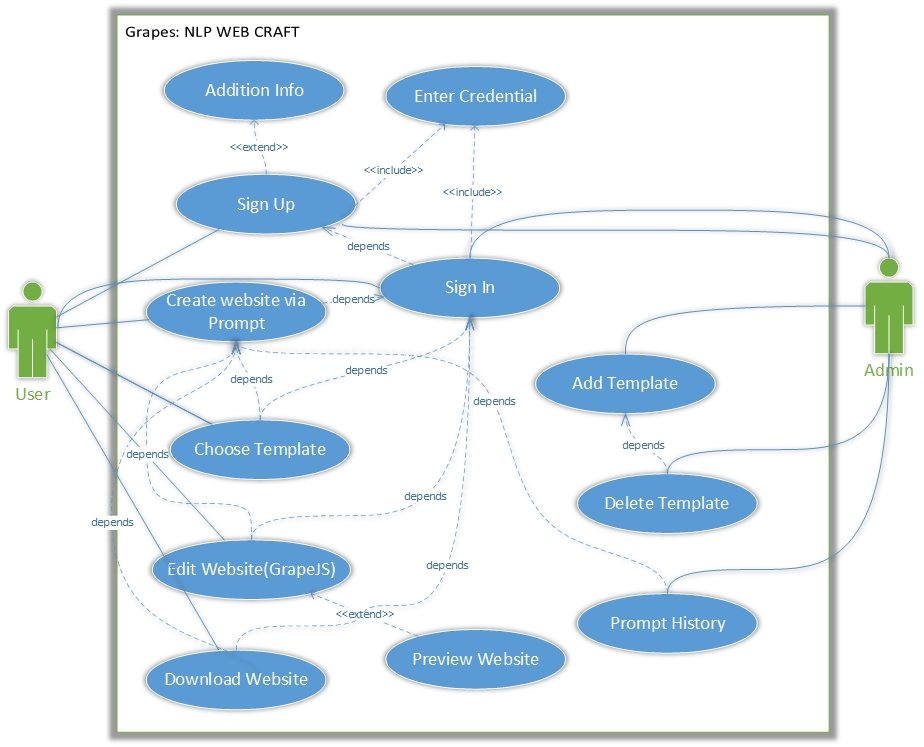
\includegraphics[width=1\textwidth]{Media/uc.jpg} % Path to your image
    \caption{Use Case Diagram}
    \label{fig:drawing1}
\end{figure}
\newpage

\begin{table}[h!]

\begin{tabular}{|p{3.5cm}|p{10cm}|} % Adjust column widths
\hline
\textbf{Use Case Name} & User Sign-Up for NLP Web Craft \\ 
\hline
\textbf{Primary Actor} & User \\ 
\hline
\textbf{Trigger} & When the "Create Account" button is pressed to register a new user. \\ 
\hline
\textbf{Goal} & Successfully create a user account to use the chatbot and website-building tools. \\ 
\hline
\textbf{Precondition} & The user is not already registered in the system. \\ 
\hline
\textbf{Postcondition} & User successfully creates an account and gains access to the system features. \\ 
\hline

\textbf{Basic Flow} & 
\begin{itemize}
    \item User opens the NLP Web Craft platform.
    \item User navigates to the "Sign-Up" subsection.
    \item System prompts for user details (name, email, password).
    \item User enters the required information.
    \item System validates the information (e.g., email, password strength).
    \item If valid, the system creates a new user account.
\end{itemize} \\ 
\hline
\textbf{Alternate Flow} & N/A \\ 
\hline
\textbf{Quality Requirements} & 
\begin{itemize}
    \item Must be available 24/7 to ensure continuous service.
    \item Must be responsive and work across all devices and screen sizes
\end{itemize} \\ 
\hline
\textbf{Exception} & 
\begin{itemize}
    \item Connection error: User should check the internet connection and retry.
    \item Session expired: User needs to re-login to continue
\end{itemize} \\ 
\hline
\end{tabular}

\caption{Use Case for User Sign-Up in NLP Web Craft} % Caption at the bottom
\end{table}

\begin{table}[h!]

\begin{tabular}{|p{3.5cm}|p{10cm}|}
\hline
\textbf{Use Case Name} & Admin Sign-Up \\ 
\hline
\textbf{Primary Actor} & Admin \\ 
\hline
\textbf{Trigger} & When the "Sign Up" button is pressed to create a new admin account. \\ 
\hline
\textbf{Goal} & Successfully create a new admin account for accessing and managing the system. \\ 
\hline
\textbf{Precondition} & The administrator is not already registered in the system. \\ 
\hline
\textbf{Postcondition} & The administrator successfully creates an admin account and gains access to the administrative features of the application. \\ 

\hline
\textbf{Basic Flow} & 
\begin{itemize}
    \item The administrator opens the car showroom application.
    \item The administrator navigates to the "Admin Sign-Up" subsection.
    \item The system prompts the administrator to provide necessary information (username, email, password, and contact details).
    \item The administrator enters the required information.
    \item The system validates the entered information (e.g., checks for valid email format, password strength).
    \item If the information is valid, the system creates a new admin account.
\end{itemize} \\ 
\hline
\textbf{Alternate Flow} & N/A \\ 
\hline

\textbf{Quality Requirements} & 
\begin{itemize}
    \item Must be available 24/7 to ensure continuous service.
    \item Must be responsive and work across all devices and screen sizes
\end{itemize} \\ 
\hline
\textbf{Exception} & 
\begin{itemize}
    \item Connection error: Admin should check the internet connection and retry.
    \item Session expired: Admin needs to re-login to continue
\end{itemize} \\ 
\hline
\end{tabular}

\caption{Use Case for Admin Sign-Up} % Caption at the bottom
\end{table}

\vspace{10pt}

\begin{table}[h!]

\begin{tabular}{|p{3.5cm}|p{10cm}|}
\hline
\textbf{Use Case Name} & User Sign-In for NLP Web Craft \\ 
\hline
\textbf{Primary Actor} & User  \\ 
\hline
\textbf{Trigger} & When the "Log In" button is pressed to access the User dashboard. \\ 
\hline
\textbf{Goal} & Successfully create a user account to use the chatbot and website-building tools. \\ 
\hline
\textbf{Precondition} & The user is not already registered in the system. \\ 
\hline
\textbf{Postcondition} & User successfully creates an account and gains access to the system features. \\ 
\hline

\textbf{Basic Flow} & 
\begin{itemize}
    \item User opens the NLP Web Craft platform.
    \item User navigates to the "Sign-Up" section.
    \item System prompts for user details (name, email, password).
    \item User enters the required information.
    \item System validates the information (e.g., email, password strength).
    \item If valid, the system creates a new user account.
\end{itemize} \\ 
\hline
\textbf{Alternate Flow} & N/A \\ 
\hline
\textbf{Quality Requirements} & 
\begin{itemize}
    \item Must be available 24/7 to ensure continuous service.
    \item Must be responsive and work across all devices and screen sizes
\end{itemize} \\ 
\hline
\textbf{Exception} & 
\begin{itemize}
    \item Connection error: User should check the internet connection and retry.
    \item Session expired: User needs to re-login to continue
\end{itemize} \\ 
\hline
\end{tabular}

\caption{Use Case: User Sign-In for NLP Web Craft}
\end{table}


\vspace{10pt}

\begin{table}[h!]

\begin{tabular}{|p{3.5cm}|p{10cm}|}
\hline
\textbf{Use Case Name} & Admin Sign-In \\ 
\hline
\textbf{Primary Actor} & Admin \\ 
\hline
\textbf{Trigger} & When the "Log In" button is pressed to access the admin dashboard. \\ 
\hline
\textbf{Goal} & Successfully log in to the admin account to manage the application. \\ 
\hline
\textbf{Precondition} & The administrator has a registered admin account. \\ 
\hline
\textbf{Postcondition} & The administrator is logged into the system and can access administrative features. \\ 

\hline
\textbf{Basic Flow} & 
\begin{itemize}
    \item The administrator navigates to the "Admin Sign-In" section.
    \item The system prompts the administrator to enter their username and password.
    \item The administrator enters the required login credentials.
    \item The system validates the credentials against the database.
    \item If the credentials are valid, the system grants access and redirects the administrator to the admin dashboard.
\end{itemize} \\ 
\hline
\textbf{Alternate Flow} & N/A \\ 
\hline

\textbf{Quality Requirements} & 
\begin{itemize}
    \item Must be available 24/7 to ensure continuous service.
    \item Must be responsive and work across all devices and screen sizes
\end{itemize} \\ 
\hline
\textbf{Exception} & 
\begin{itemize}
    \item Connection error: Admin should check the internet connection and retry.
    \item Session expired: Admin needs to re-login to continue
\end{itemize} \\ 

\hline
\end{tabular}
\caption{Use Case for Admin Sign-In}
\end{table}
\clearpage
\vspace{10pt}
\clearpage
\begin{table}[h!]

\begin{tabular}{|p{3.5cm}|p{10cm}|}
\hline
\textbf{Use Case Name} & Create Website Via Prompt \\ 
\hline
\textbf{Primary Actor} & User \\ 
\hline
\textbf{Trigger} & When the "Create Website" button is pressed after selecting a type and writing a prompt. \\ 
\hline
\textbf{Goal} & Successfully create a website based on the user’s prompt and selected type. \\ 
\hline
\textbf{Precondition} & The user is logged in to the system. \\ 
\hline
\textbf{Postcondition} & The website is created based on the user’s specifications and is accessible for further editing. \\ 
\hline

\textbf{Basic Flow} & 
\begin{itemize}
    
    \item The system presents three options for website types: E-commerce, Blog, and Portfolio.
    \item The system prompts the user to enter a description or prompt for the website.
    \item The user writes and submits the prompt.
\end{itemize} \\ 
\hline
\textbf{Alternate Flow} & N/A \\ 
\hline
\textbf{Quality Requirements} & 
\begin{itemize}
    \item Must be available 24/7 to ensure continuous service.
    \item Must be responsive and work across all devices and screen sizes
\end{itemize} \\ 

\textbf{Exception} & 
\begin{itemize}
    \item Connection error: User should check the internet connection and retry.
    \item Session expired: User needs to re-login to continue
\end{itemize} \\ 
\hline
\end{tabular}
\caption{Use Case for Create Website Via Prompt}
\end{table}
\clearpage
\vspace{10pt}

\begin{table}[h!]

\begin{tabular}{|p{3.5cm}|p{10cm}|}
\hline
\textbf{Use Case Name} & Choose Template Theme \\ 
\hline
\textbf{Primary Actor} & User \\ 
\hline
\textbf{Trigger} & When the "Select Template" button is pressed to choose a template for the website. \\ 
\hline
\textbf{Goal} & Successfully choose a template that fits the user's needs. \\ 
\hline
\textbf{Precondition} & The user has created a website and is ready to choose a template. \\ 
\hline
\textbf{Postcondition} & The user successfully selects a template, and the website is updated accordingly. \\ 

\hline
\textbf{Basic Flow} & 
\begin{itemize}
    \item The user opens the template selection section of the NLP Web Craft platform.
    \item The system presents a gallery of available templates.
    \item The user browses through the templates and selects one.
    \item The system updates the website with the selected template.
\end{itemize} \\ 
\hline
\textbf{Alternate Flow} & N/A \\ 
\hline
\textbf{Quality Requirements} & 
\begin{itemize}
    \item Must be available 24/7 to ensure continuous service.
    \item Must be responsive and work across all devices and screen sizes
\end{itemize} \\ 
\hline
\textbf{Exception} & 
\begin{itemize}
    \item Connection error: User should check the internet connection and retry.
    \item Session expired: User needs to re-login to continue
\end{itemize} \\ 
\hline
\end{tabular}

\caption{Use Case for Choose Template}
\end{table}
\clearpage
\vspace{10pt}

\begin{table}[h!]

\begin{tabular}{|p{3.5cm}|p{10cm}|}
\hline
\textbf{Use Case Name} & Customize Website \\ 
\hline
\textbf{Primary Actor} & User \\ 
\hline
\textbf{Trigger} & When the "Edit" button is pressed after selecting a website template. \\ 
\hline
\textbf{Goal} & Successfully customize the website according to user preferences. \\ 
\hline
\textbf{Precondition} & The user has selected a template for the website. \\ 
\hline
\textbf{Postcondition} & The website is customized according to user preferences and is saved for future access. \\ 
\hline

\textbf{Basic Flow} & 
\begin{itemize}
    \item The user navigates to the website dashboard.
    \item The user selects the website they wish to edit.
    \item The system opens the GrapeJS editor for the selected website.
    \item The user customizes the website using the editing tools available in GrapeJS.
    \item The user saves the changes made to the website.
\end{itemize} \\ 
\hline
\textbf{Alternate Flow} & N/A \\ 
\hline
\textbf{Quality Requirements} & 
\begin{itemize}
    \item Must be available 24/7 to ensure continuous service.
    \item Must be responsive and work across all devices and screen sizes
\end{itemize} \\ 
\hline
\textbf{Exception} & 
\begin{itemize}
    \item Connection error: User should check the internet connection and retry.
    \item Customization failed: User must refresh the browser and try the customization again
\end{itemize} \\ 
\hline
\end{tabular}

\caption{Use Case for Customize Website}
\end{table}
\clearpage
% Edit Website Use Case
\begin{table}[h!]

\begin{tabular}{|p{3.5cm}|p{10cm}|}
\hline
\textbf{Use Case Name} & Edit Website Using GrapeJS \\ 
\hline
\textbf{Primary Actor} & User \\ 
\hline
\textbf{Trigger} & When the "Edit" button is pressed to open the GrapeJS editor for customization. \\ 
\hline
\textbf{Goal} & Successfully modify and customize the website using GrapeJS editor. \\ 
\hline
\textbf{Precondition} & The user has selected a template for their website. \\ 
\hline
\textbf{Postcondition} & The changes made to the website are saved, and the user can preview the updated website. \\ 
\hline
\textbf{Basic Flow} & 
\begin{itemize}
    \item The user navigates to the "Edit Website" section using GrapeJS.
    \item The system loads the selected template into the GrapeJS editor.
    \item The user interacts with the GrapeJS interface to modify elements (text, images, layout).
    \item The user can add, remove, or rearrange components within the website.
   
\end{itemize} \\ 
\hline
\textbf{Alternate Flow} & N/A \\ 
\hline
\textbf{Quality Requirements} & 
\begin{itemize}
    \item Must be available 24/7 to ensure continuous service.
    \item Must be responsive and work across all devices and screen sizes
\end{itemize} \\ 
\hline
\textbf{Exception} & 
\begin{itemize}
    \item Connection error: User should check the internet connection and retry.
    \item Session expired: User needs to re-login to continue
\end{itemize} \\ 
\hline
\end{tabular}

\caption{Use Case: Edit Website Using GrapeJS}
\end{table}
\clearpage
% Download Website Use Case
\begin{table}[h!]

\begin{tabular}{|p{3.5cm}|p{10cm}|}
\hline
\textbf{Use Case Name} & Download Website \\ 
\hline
\textbf{Primary Actor} & User  \\ 
\hline
\textbf{Trigger} & When the "Download" button is pressed to download the completed website files. \\ 
\hline
\textbf{Goal} & Successfully download the website files in a zip format. \\ 
\hline
\textbf{Precondition} & The user has edited and finalized their website using the GrapeJS editor. \\ 
\hline
\textbf{Postcondition} & The website files are downloaded to the user's device. \\ 
\hline
\textbf{Basic Flow} & 
\begin{itemize}
    \item The user navigates to the "Download Website" section.
    \item The system presents an option to download the completed website.
    \item The user clicks the "Download" button.
    \item The system compiles the website files (HTML, CSS, JavaScript, assets) into a zip file.
    \item The system prompts the user to save the zip file to their device.
\end{itemize} \\ 
\hline
\textbf{Alternate Flow} & N/A \\ 
\hline
\textbf{Quality Requirements} & 
\begin{itemize}
    \item Must be available 24/7 to ensure continuous service.
    \item Must ensure that all necessary files are included in the zip package.
\end{itemize} \\ 
\hline
\textbf{Exception} & 
\begin{itemize}
    \item Connection error: User should check the internet connection and retry.
    \item File Download failed: User needs to check the file format and size before uploading
\end{itemize} \\ 
\hline
\end{tabular}

\caption{Use Case: Download Website}
\end{table}
\clearpage
% Add Template Use Case
\begin{table}[h!]

\begin{tabular}{|p{3.5cm}|p{10cm}|}
\hline
\textbf{Use Case Name} & Add Template \\ 
\hline
\textbf{Primary Actor} & Admin \\ 
\hline
\textbf{Trigger} & When the "Add Template" button is pressed to upload a new template. \\ 
\hline
\textbf{Goal} & Successfully add a new template to the system for user selection. \\ 
\hline
\textbf{Precondition} & The admin is logged into the system with appropriate privileges. \\ 
\hline
\textbf{Postcondition} & The new template is available for users to select when creating their websites. \\ 
\hline
\textbf{Basic Flow} & 
\begin{itemize}
    \item The admin opens the NLP Web Craft platform.
    \item The admin navigates to the "Add Template" section.
    \item The system prompts the admin to upload the template files (HTML, CSS, JavaScript, assets).
    \item The admin uploads the necessary files and enters relevant details (template name, description, category).
    \item The system validates the uploaded files and details.
\end{itemize} \\ 
\hline
\textbf{Alternate Flow} & N/A \\ 
\hline
\textbf{Quality Requirements} & 
\begin{itemize}
    \item Must be available 24/7 to ensure continuous service.
    \item Must be responsive and work across all devices and screen sizes
\end{itemize} \\ 
\hline
\textbf{Exception} & 
\begin{itemize}
    \item Connection error: Admin should check the internet connection and retry.
    \item File upload failed: Admin needs to check the file format and size before uploading
\end{itemize} \\ 
\hline
\end{tabular}

\caption{Use Case: Add Template}
\end{table}
\clearpage
% Delete Template Use Case
\begin{table}[h!]

\begin{tabular}{|p{3.5cm}|p{10cm}|}
\hline
\textbf{Use Case Name} & Delete Template \\ 
\hline
\textbf{Primary Actor} & Admin \\ 
\hline
\textbf{Trigger} & When the "Delete" button is pressed to remove an existing template from the system. \\ 
\hline
\textbf{Goal} & Successfully delete a template from the system. \\ 
\hline
\textbf{Precondition} & The admin is logged into the system with appropriate privileges. \\ 
\hline
\textbf{Postcondition} & The selected template is removed from the system and is no longer available for user selection. \\ 
\hline
\textbf{Basic Flow} & 
\begin{itemize}
    \item The admin navigates to the "Manage Templates" section.
    \item The system displays a list of existing templates.
    \item The admin selects the template they wish to delete.
    \item The system prompts the admin to confirm the deletion.

\end{itemize} \\ 
\hline
\textbf{Alternate Flow} & N/A \\ 
\hline
\textbf{Quality Requirements} & 
\begin{itemize}
    \item Must be available 24/7 to ensure continuous service.
    \item Must be responsive and work across all devices and screen sizes
\end{itemize} \\ 
\hline
\textbf{Exception} & 
\begin{itemize}
    \item Connection error: Admin should check the internet connection and retry.
    \item Session expired: Admin needs to re-login to continue
\end{itemize} \\ 
\hline
\end{tabular}

\caption{Use Case: Delete Template}
\end{table}
\clearpage
% View Prompt History Use Case
\begin{table}[h!]

\begin{tabular}{|p{3.5cm}|p{10cm}|}
\hline
\textbf{Use Case Name} & View Prompt History \\ 
\hline
\textbf{Primary Actor} & Admin\\ 
\hline
\textbf{Trigger} & When the "View Prompt History" button is pressed to access the list of previous prompts. \\ 
\hline
\textbf{Goal} & Successfully access and view the history of prompts used in the system. \\ 
\hline
\textbf{Precondition} & The admin is logged into the system with appropriate privileges. \\ 
\hline
\textbf{Postcondition} & The admin can review the history of prompts and their usage. \\ 
\hline
\textbf{Basic Flow} & 
\begin{itemize}
    \item The admin navigates to the "Prompt History" section.
    \item The system displays a list of all previous prompts used in the system.
    \item The admin can view details about each prompt (date, time, user who initiated, etc.).
\end{itemize} \\ 
\hline
\textbf{Alternate Flow} & N/A \\ 
\hline
\textbf{Quality Requirements} & 
\begin{itemize}
    \item Must be available 24/7 to ensure continuous service.
    \item Must be responsive and work across all devices and screen sizes
\end{itemize} \\ 
\hline
\textbf{Exception} & 
\begin{itemize}
    \item Connection error: Admin should check the internet connection and retry.
    \item Session expired: Admin needs to re-login to continue
\end{itemize} \\ 
\hline
\end{tabular}

\caption{Use Case: View Prompt History}
\end{table}
\clearpage

\chapter{\Huge \bfseries Design Specification}
\fancyhead[L]{Chapter 2. Design Specification} % Left-aligned header
\renewcommand{\headrulewidth}{0.4pt} % Optional: add a line 

\section{User Interphase Design}
\subsection{WireFrames}
\begin{figure}[ht]
    \centering
    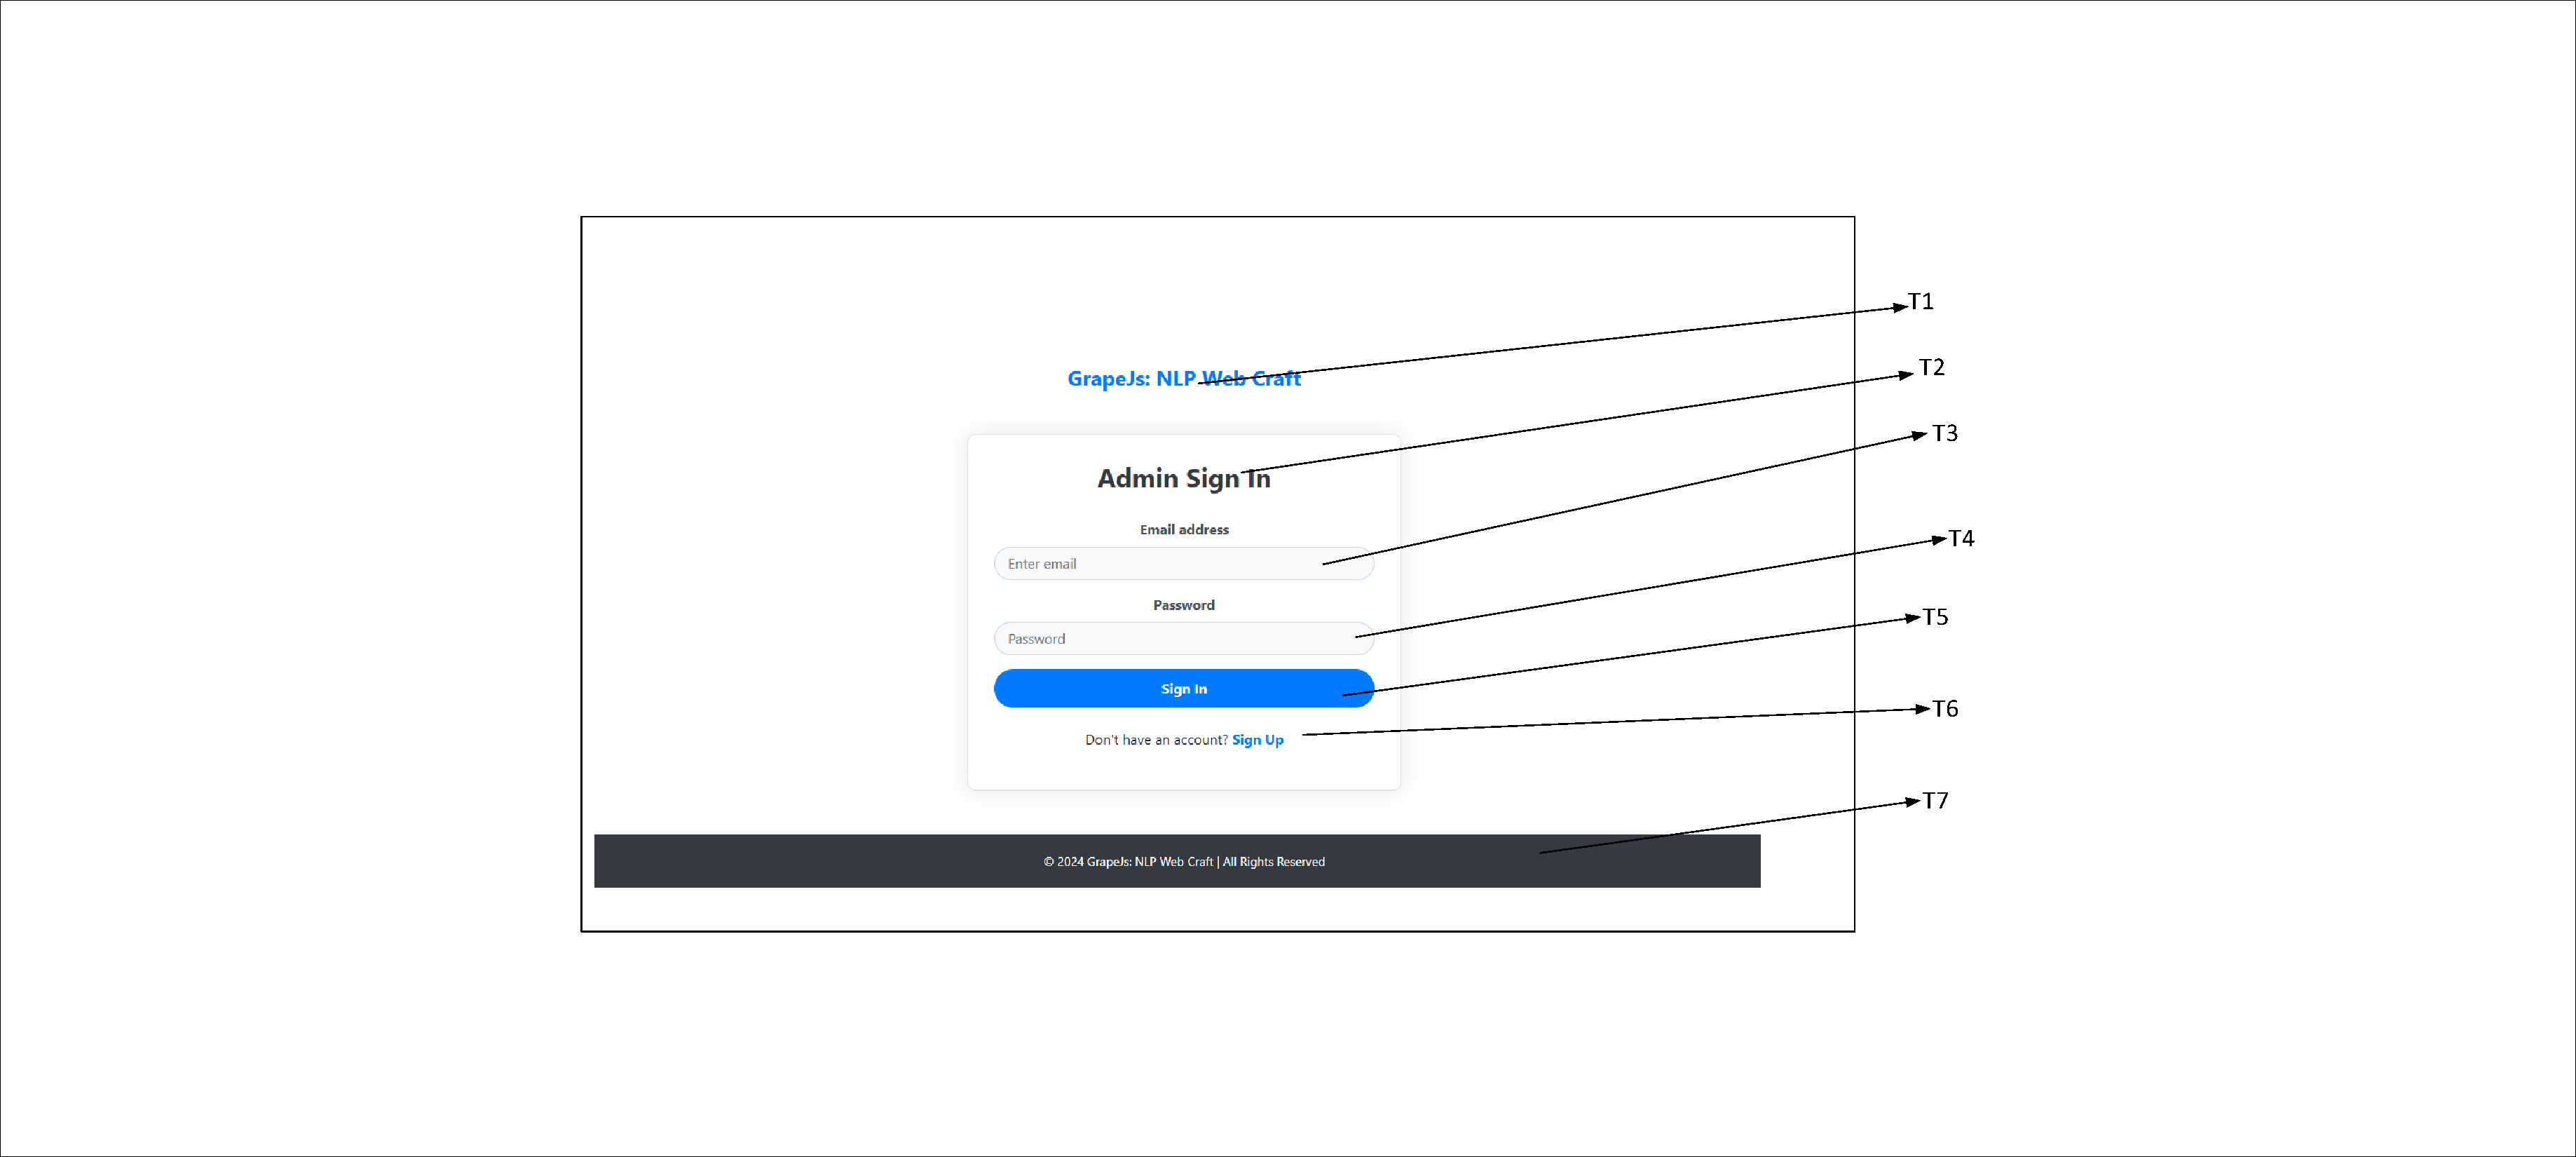
\includegraphics[width=1\textwidth, trim=10cm 5cm 10cm 5cm, clip]{Media/1 .pdf} % Path to your image
    \caption{WireFrame: Admin Sgin In}
    \label{fig:drawing1}
\end{figure}



\begin{table}[h!]
    \centering
    \begin{tabular}{|c|p{10cm}|}
        \hline
        \textbf{Element} & \textbf{Description} \\
        \hline
        T1 & As an admin, I shall view the logo. \\
        \hline
        T2 & As an admin, I shall view the Sign in page. \\
        \hline
        T3 & As an admin, I shall enter my email ID. \\
        \hline
        T4 & As an admin, I shall enter my password. \\
        \hline
        T5 & As an admin, I shall click on the Sign in button. \\
        \hline
        T6 & As an admin, I shall click on the Sign up link. \\
        \hline
        T7 & As an admin, I shall view the "All rights reserved" label. \\
        \hline
    \end{tabular}
    \caption{WireFrame: Admin Sgin In}
    \label{tab:admin_actions}
\end{table}


\begin{figure}[ht]
    \centering
    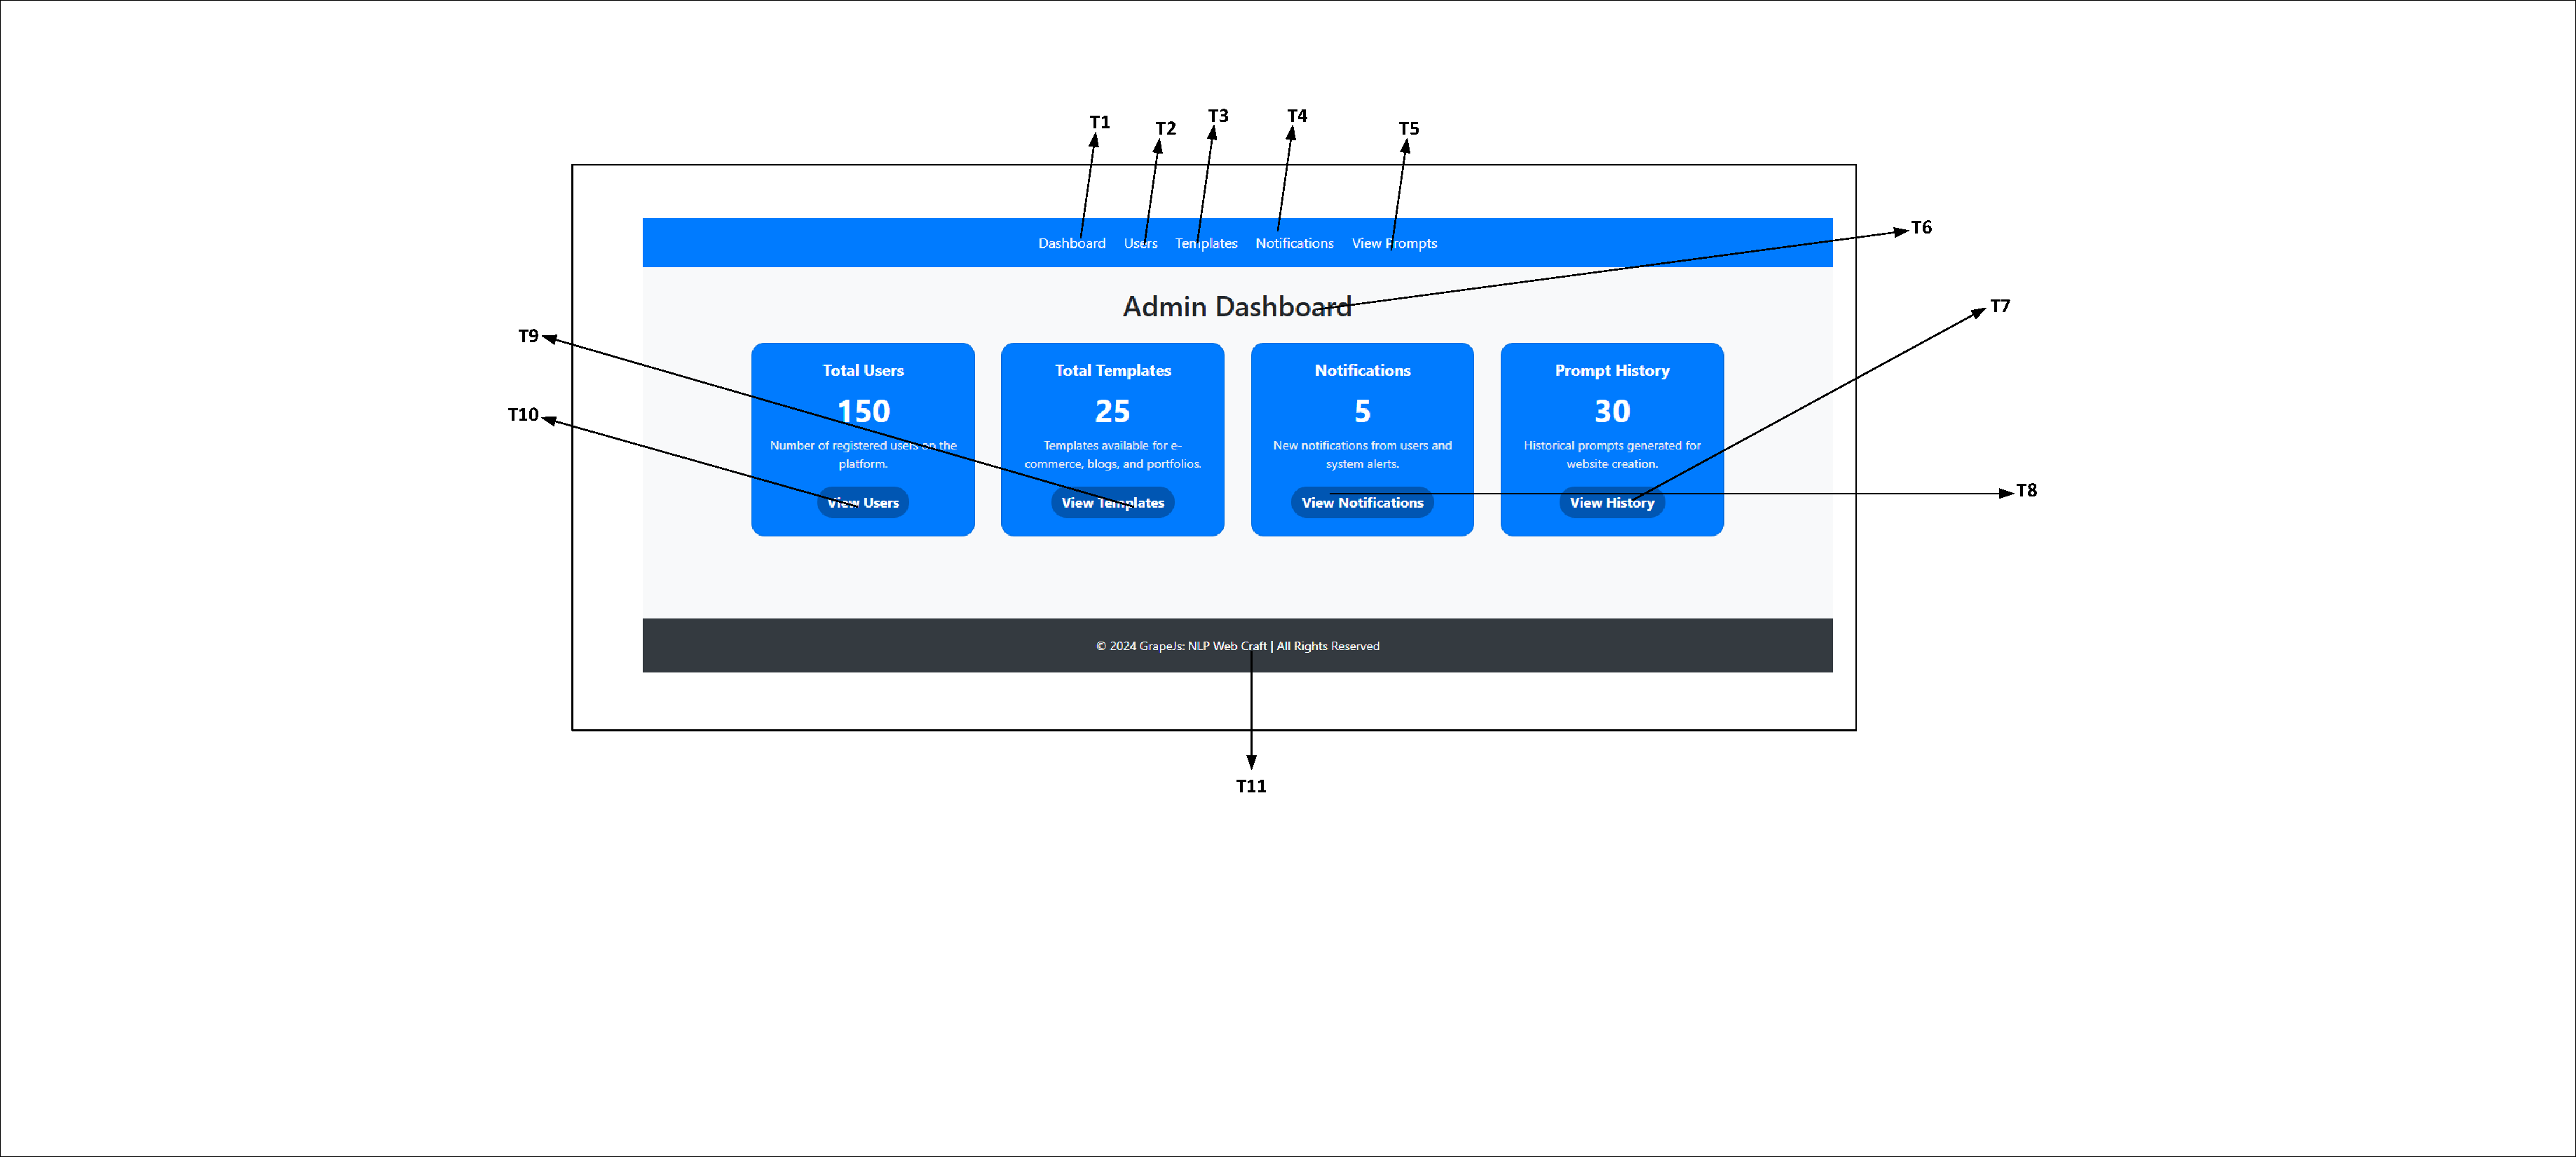
\includegraphics[width=1\textwidth, trim=10cm 10cm 10cm 2cm, clip]{Media/2.pdf} % Path to your image
    \caption{WireFrame: Admin Dashboard}
    \label{fig:drawing1}
\end{figure}

\begin{table}[h!]
    \centering
    \begin{tabular}{|c|p{10cm}|}
        \hline
        \textbf{Element} & \textbf{Description} \\
        \hline
        T1 & As an admin, I shall click on the dashboard. \\
        \hline
        T2 & As an admin, I shall click on users. \\
        \hline
        T3 & As an admin, I shall click on templates. \\
        \hline
        T4 & As an admin, I shall click on notifications. \\
        \hline
        T5 & As an admin, I shall click on view templates. \\
        \hline
        T6 & As an admin, I shall view the admin Dashboard label. \\
        \hline
        T7 & As an admin, I shall click on view users. \\
        \hline
        T8 & As an admin, I shall click on view templates. \\
        \hline
        T9 & As an admin, I shall click on view notifications. \\
        \hline
        T10 & As an admin, I shall click on view history. \\
        \hline
        T11 & As an admin, I shall view the "All rights reserved" label. \\
        \hline
    \end{tabular}
    \caption{WireFrame: Admin Dashboard}
    \label{tab:admin_actions}
\end{table}

\begin{figure}[ht]
    \centering
    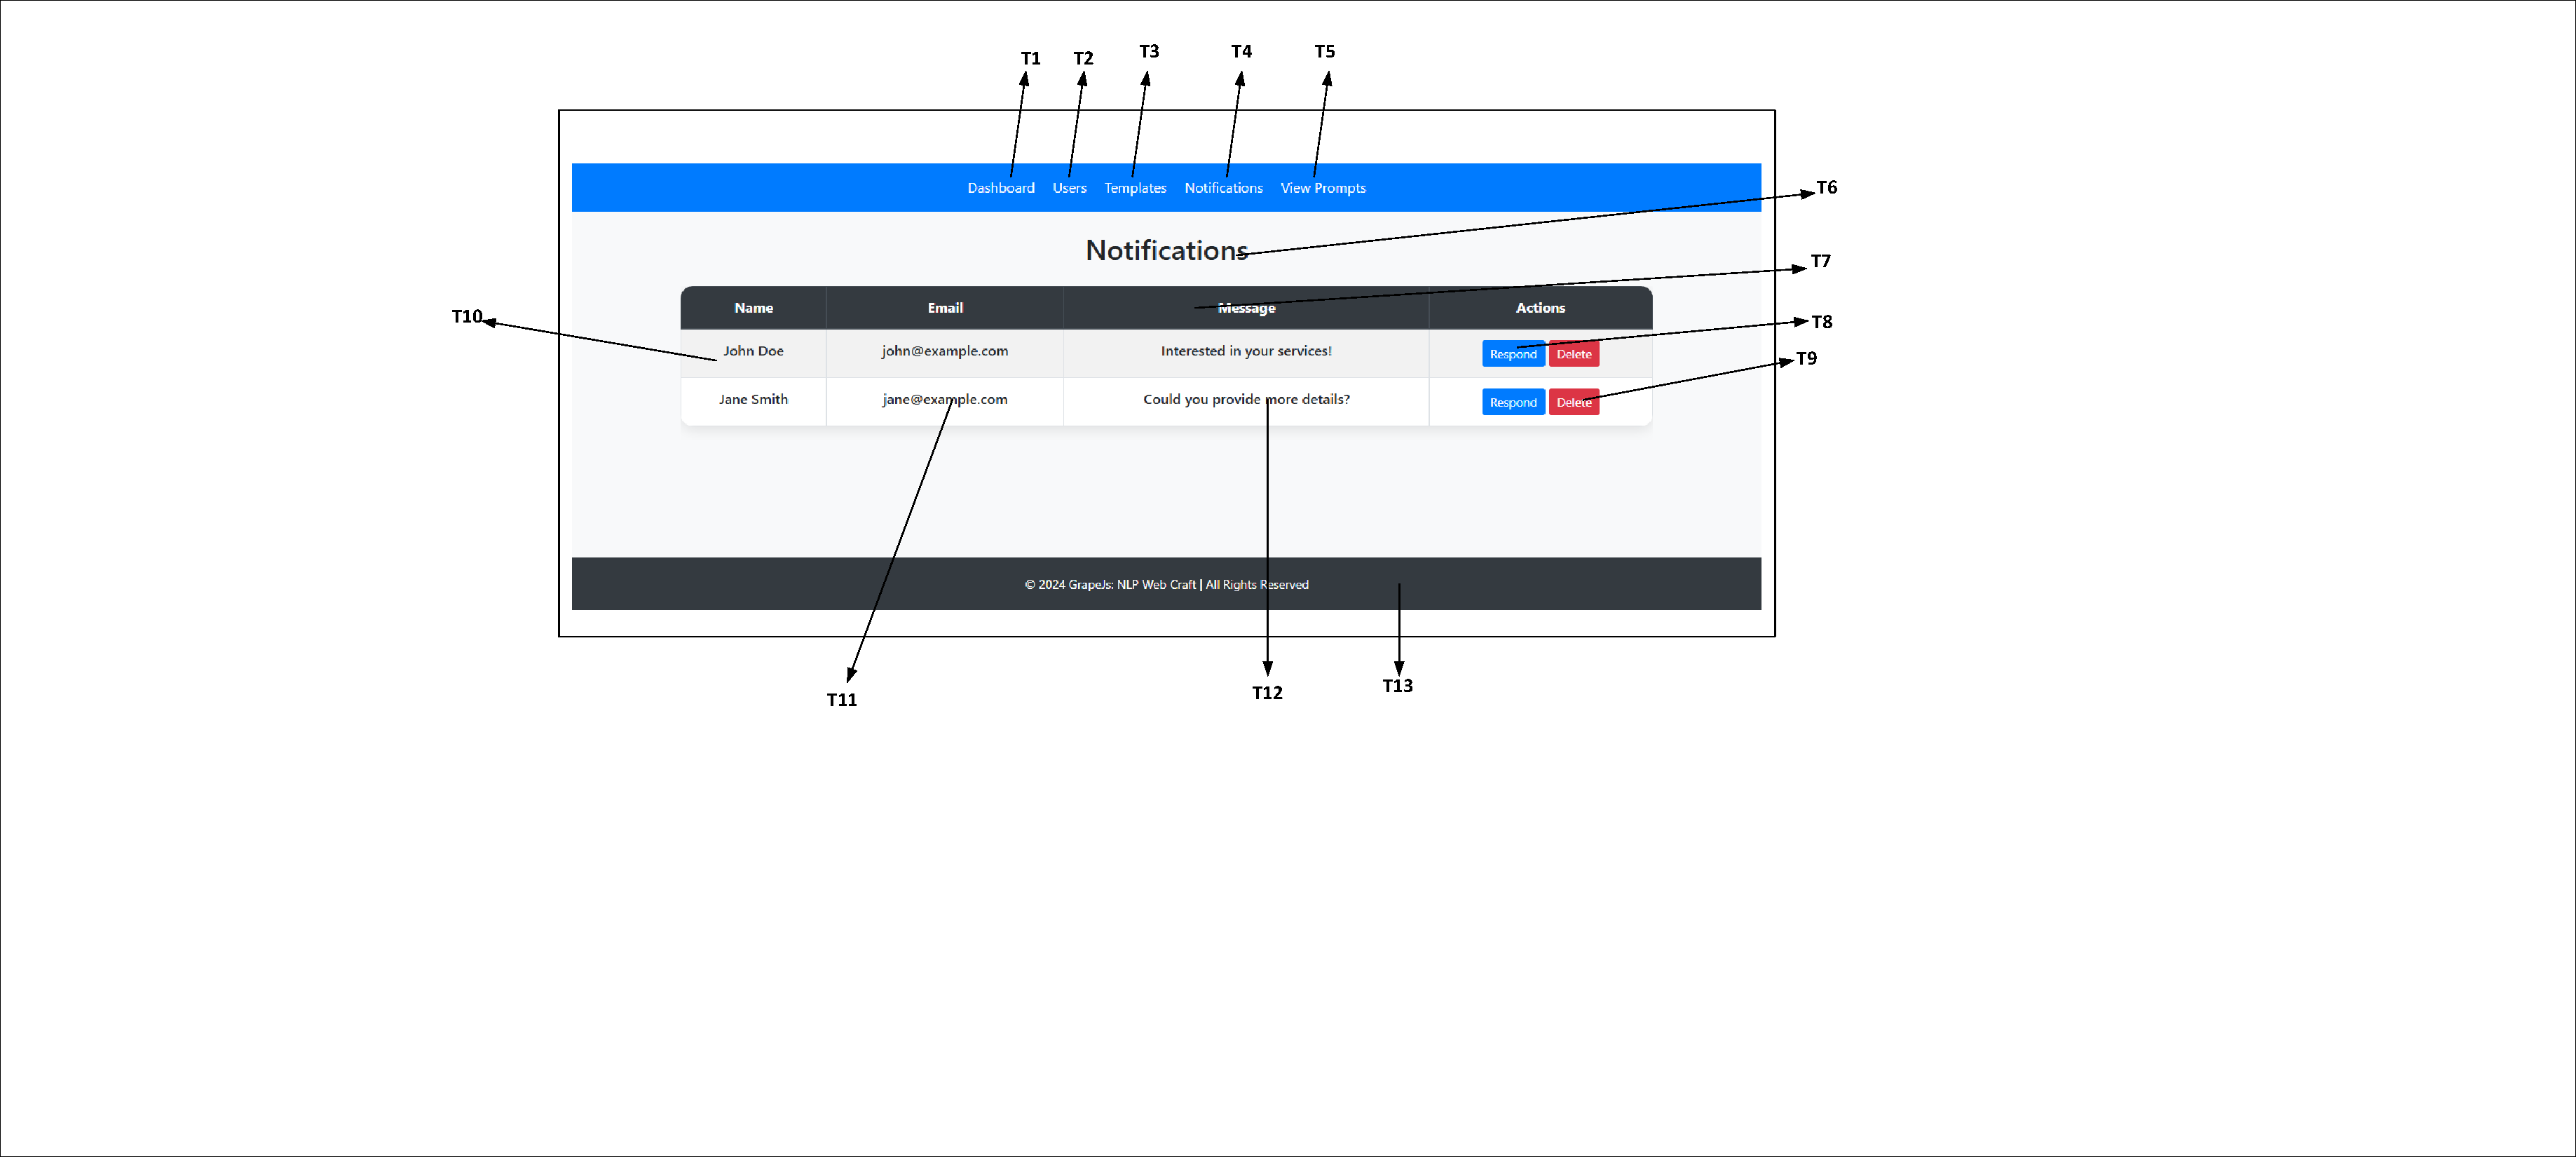
\includegraphics[width=1\textwidth, trim=10cm 9cm 14cm 0cm, clip]{Media/3.pdf} % Path to your image
    \caption{WireFrame: Admin Notification}
    \label{fig:drawing1}
\end{figure}
\begin{table}[h!]
    \centering
    \begin{tabular}{|c|p{10cm}|}
        \hline
        \textbf{Element} & \textbf{Description} \\
        \hline
        T1 & As an admin, I shall click on the dashboard. \\
        \hline
        T2 & As an admin, I shall click on users. \\
        \hline
        T3 & As an admin, I shall click on templates. \\
        \hline
        T4 & As an admin, I shall click on notifications. \\
        \hline
        T5 & As an admin, I shall click on view prompts. \\
        \hline
        T6 & As an admin, I shall view the "Notifications" label. \\
        \hline
        T7 & As an admin, I shall click on the view user description row. \\
        \hline
        T8 & As an admin, I shall click on the respond button. \\
        \hline
        T9 & As an admin, I shall click on the delete button. \\
        \hline
        T10 & As an admin, I shall click on the view user name. \\
        \hline
        T11 & As an admin, I shall view the user email. \\
        \hline
        T12 & As an admin, I shall view the user message. \\
        \hline
        T13 & As an admin, I shall view the "All rights reserved" label. \\
        \hline
    \end{tabular}
    \caption{WireFrame: Admin Notification}
    \label{tab:admin_user_management_actions}
\end{table}
\begin{figure}[ht]
    \centering
    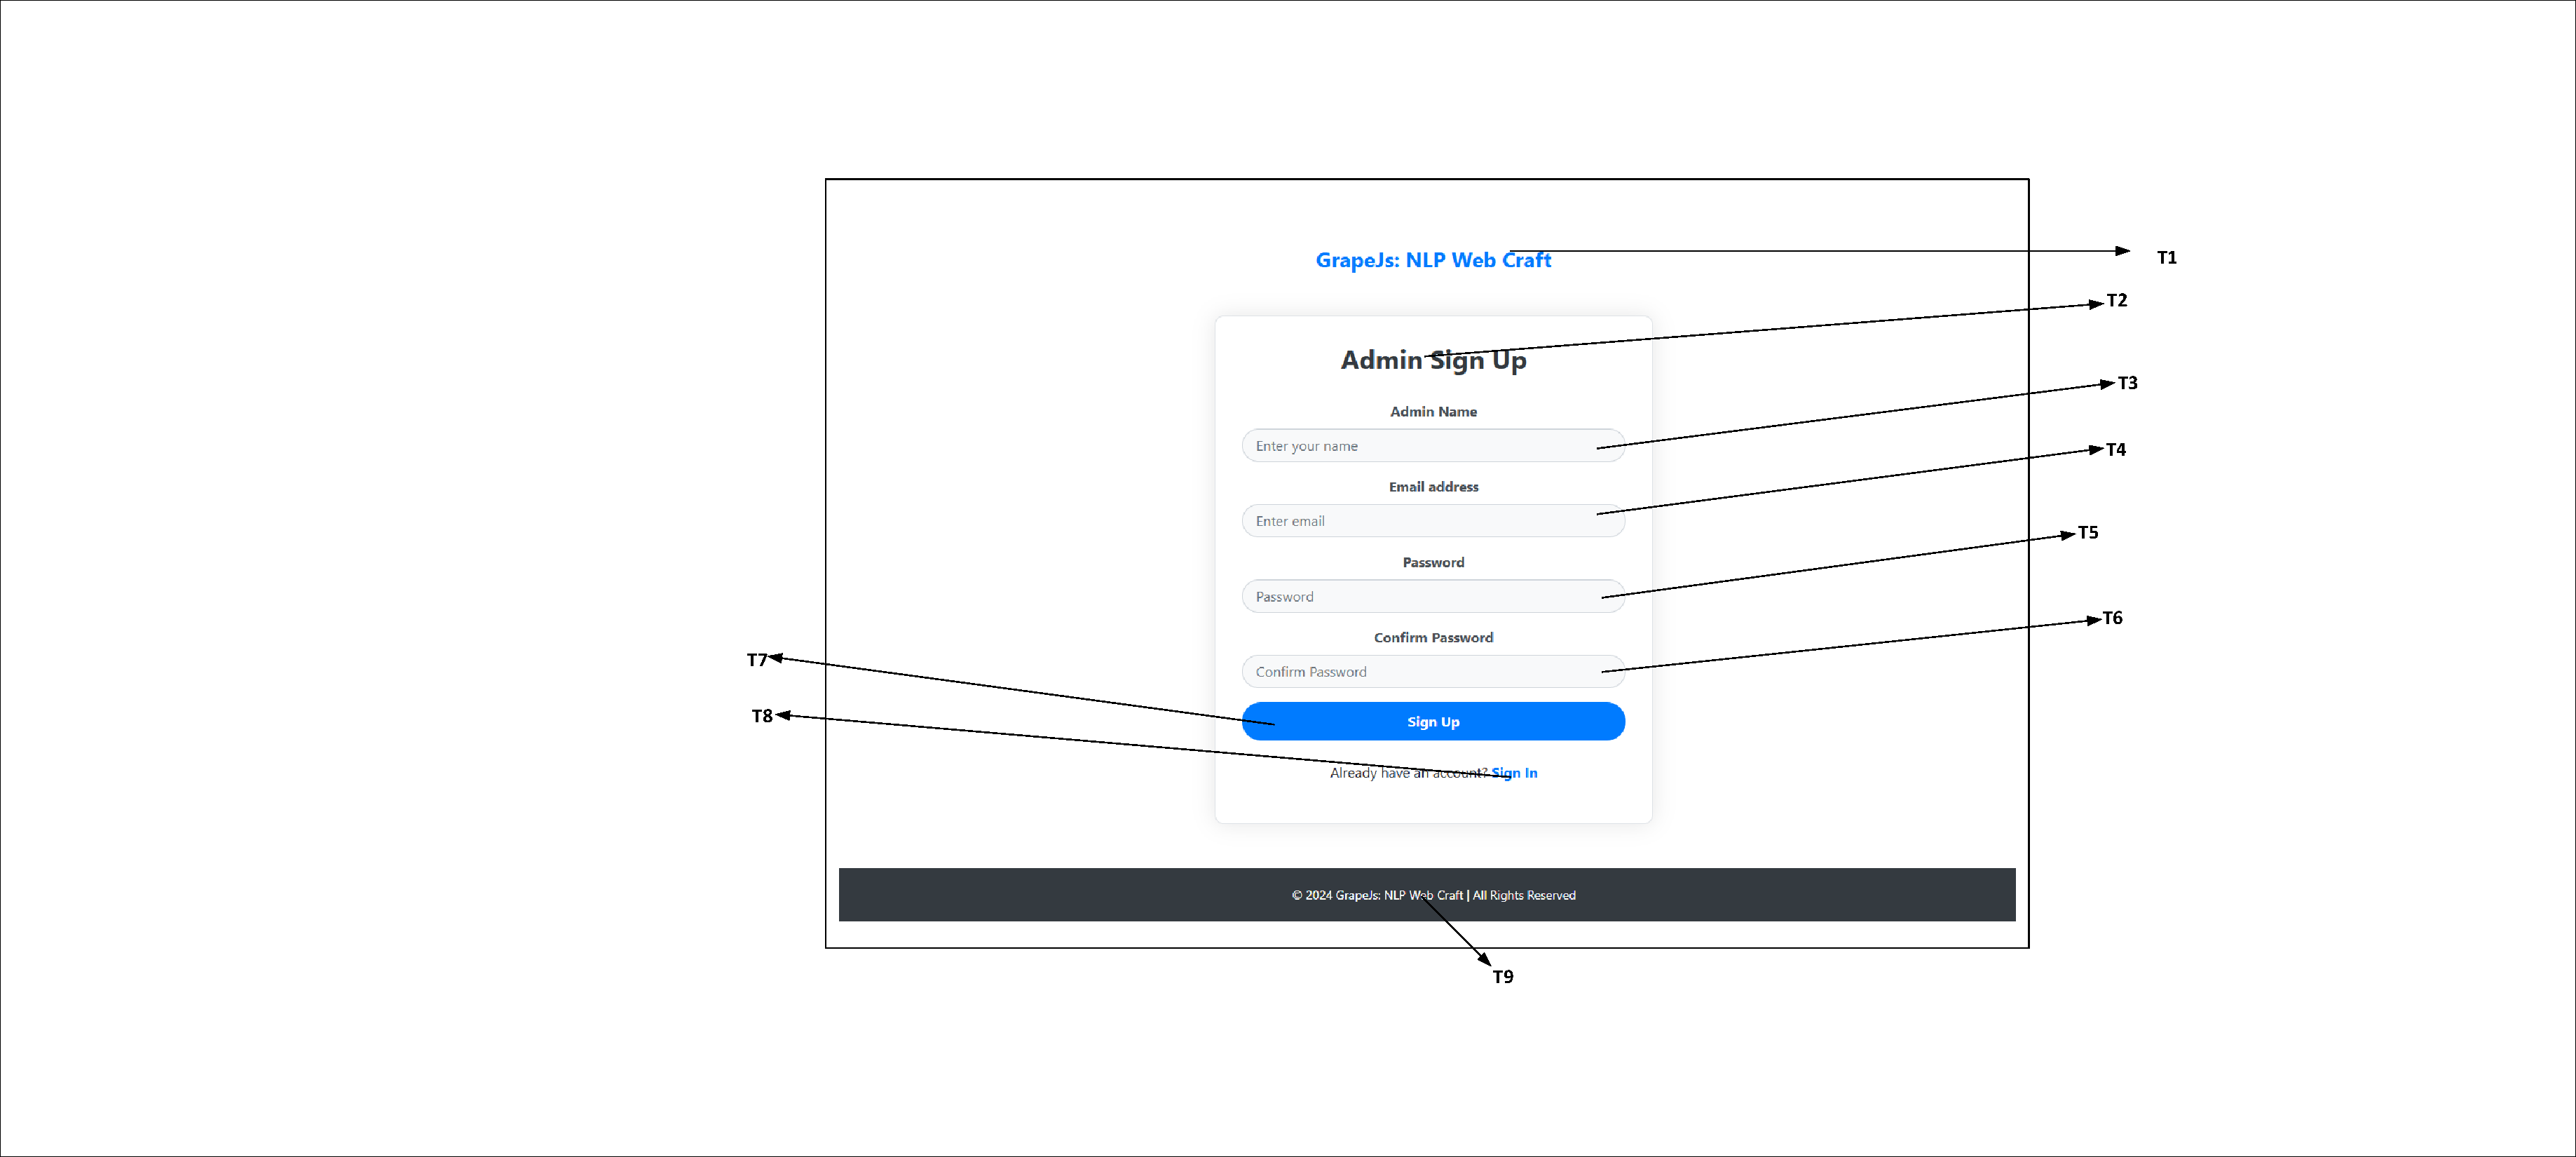
\includegraphics[width=1\textwidth, trim=10cm 2cm 8cm 0cm, clip]{Media/4.pdf} % Path to your image
    \caption{WireFrame: Admin Sign In}
    \label{fig:drawing1}
\end{figure}
 \begin{table}[h!]
    \centering
    \begin{tabular}{|c|p{10cm}|}
        \hline
        \textbf{Element} & \textbf{Description} \\
        \hline
        T1 & As an admin, I shall view the GrapesJS NLP Web Craft label. \\
        \hline
        T2 & As an admin, I shall view the Sign Up page. \\
        \hline
        T3 & As an admin, I shall enter my name. \\
        \hline
        T4 & As an admin, I shall enter my email address. \\
        \hline
        T5 & As an admin, I shall enter my password. \\
        \hline
        T6 & As an admin, I shall enter my confirm password. \\
        \hline
        T7 & As an admin, I shall click on the sign up button. \\
        \hline
        T8 & As an admin, I shall click on the sign in link. \\
        \hline
        T9 & As an admin, I shall view the "All rights reserved" label. \\
        \hline
    \end{tabular}
    \caption{WireFrame: Admin Sign In}
    \label{tab:admin_signup_actions}
\end{table}
\begin{figure}[ht]
    \centering
    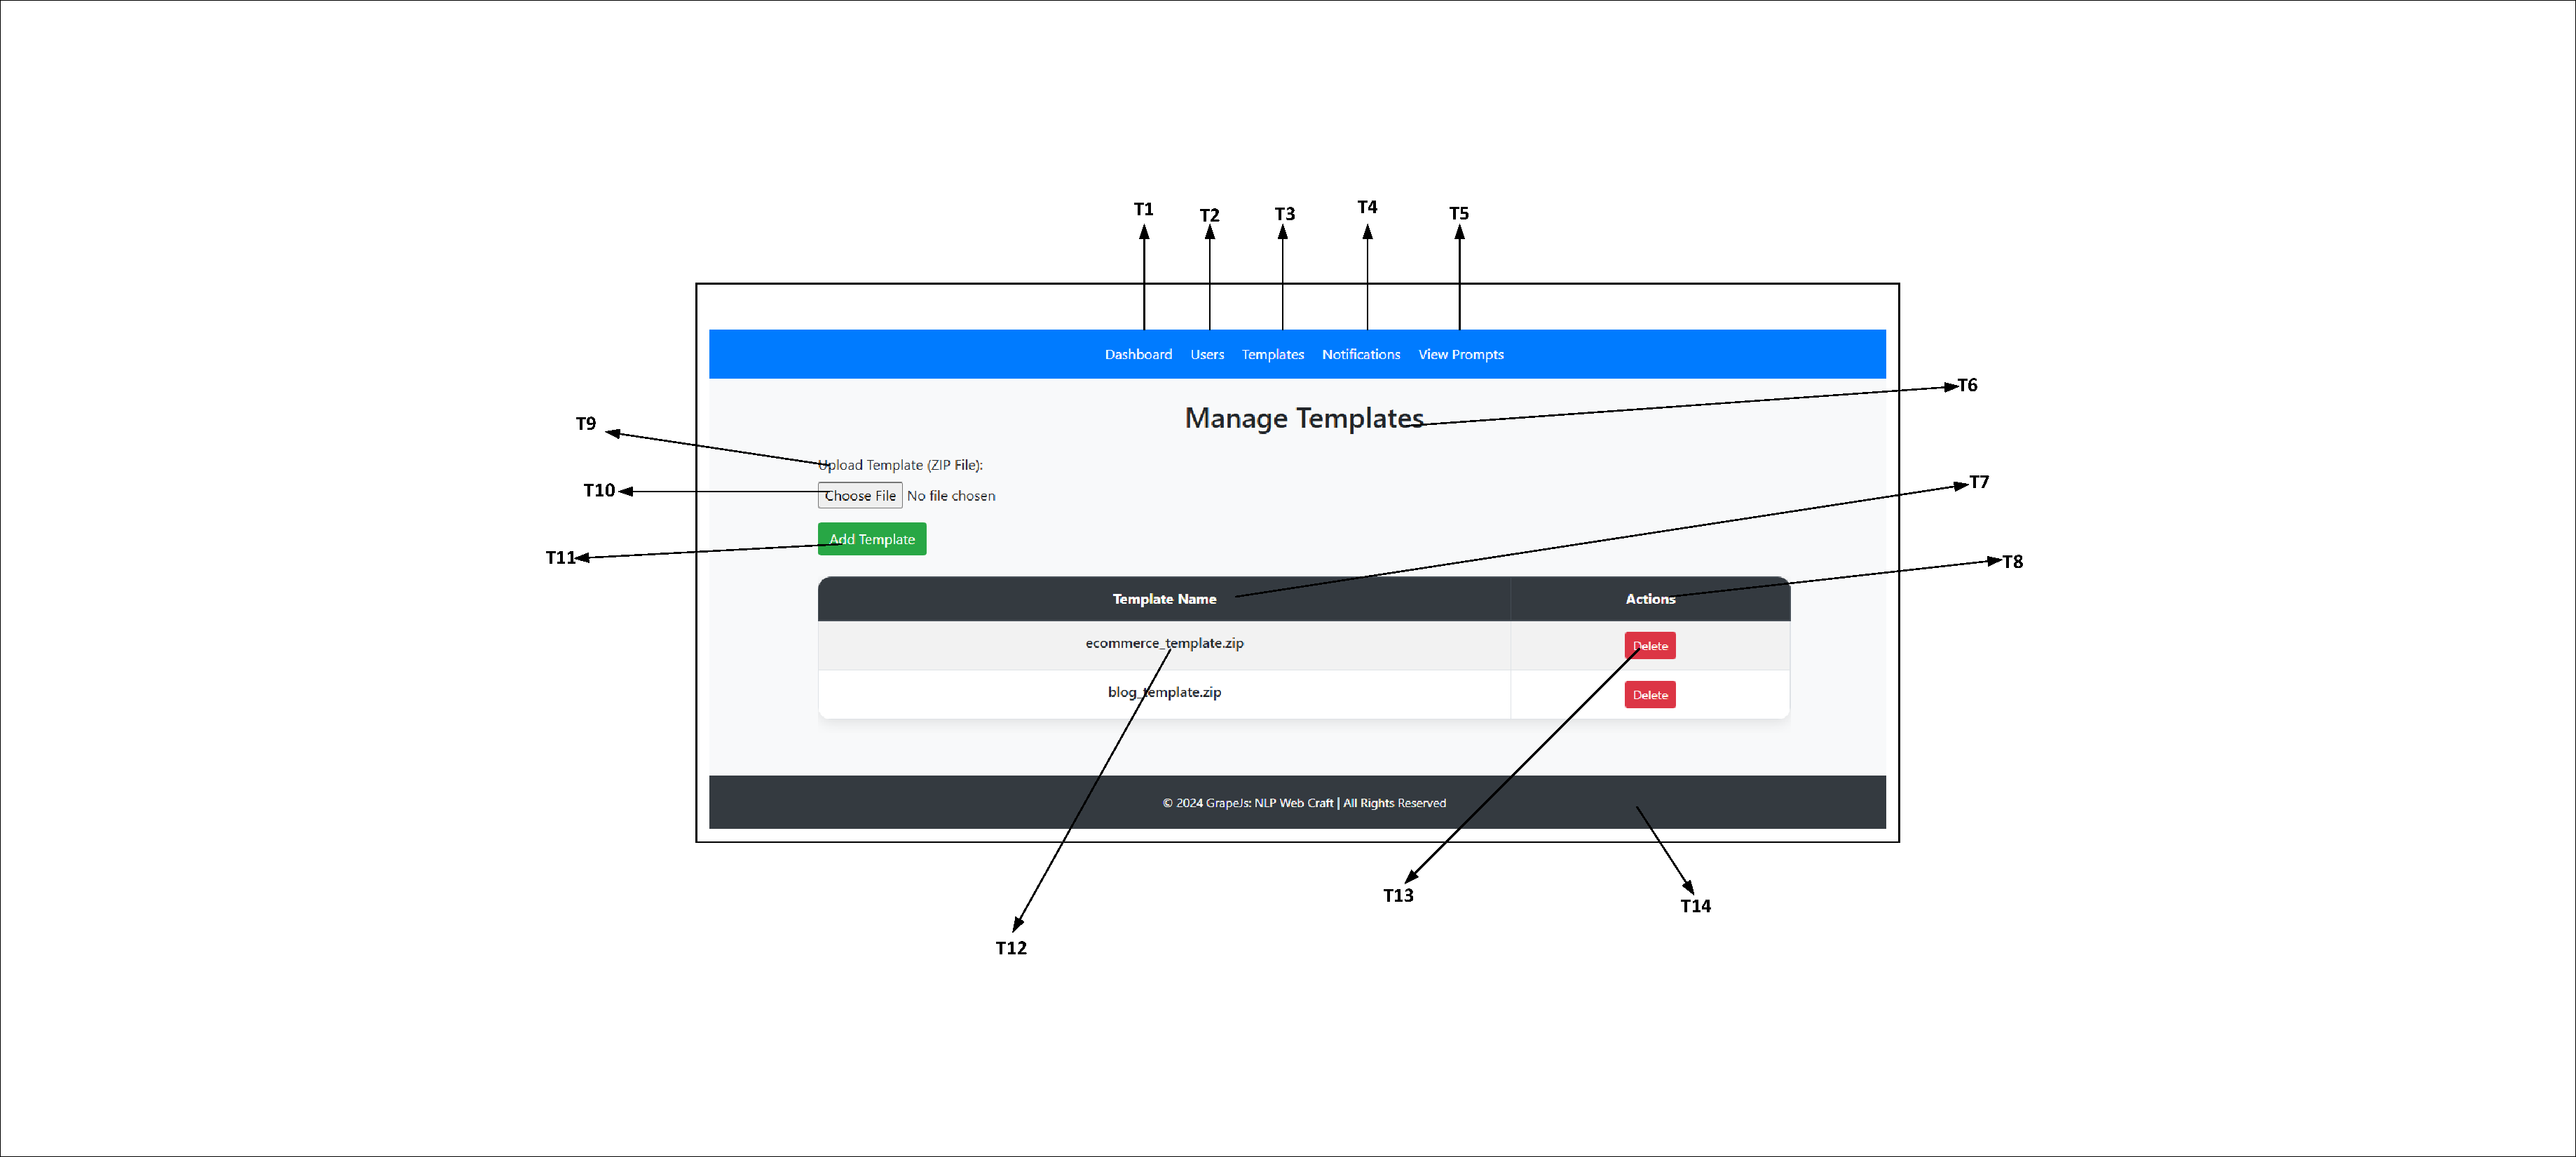
\includegraphics[width=1\textwidth, trim=10cm 4cm 10cm 4cm, clip]{Media/5.pdf} % Path to your image
    \caption{WireFrame: Admin Manage Template}
    \label{fig:drawing1}
\end{figure} 
\begin{table}[h!]
    \centering
    \begin{tabular}{|c|p{10cm}|}
        \hline
        \textbf{Element} & \textbf{Description} \\
        \hline
        T1 & As an admin, I shall click on the dashboard. \\
        \hline
        T2 & As an admin, I shall click on users. \\
        \hline
        T3 & As an admin, I shall click on templates. \\
        \hline
        T4 & As an admin, I shall click on notifications. \\
        \hline
        T5 & As an admin, I shall click on view prompts. \\
        \hline
        T6 & As an admin, I shall view the "Manage templates" label. \\
        \hline
        T7 & As an admin, I shall view the "Template name" label. \\
        \hline
        T8 & As an admin, I shall view the "Action" label. \\
        \hline
        T9 & As an admin, I shall view the "Upload template" label. \\
        \hline
        T10 & As an admin, I shall click on the "Choose file" button. \\
        \hline
        T11 & As an admin, I shall click on the "Add template" button. \\
        \hline
        T12 & As an admin, I shall view the template name. \\
        \hline
        T13 & As an admin, I shall click on the delete button. \\
        \hline
        T14 & As an admin, I shall view the "All rights reserved" label. \\
        \hline
    \end{tabular}
    \caption{WireFrame: Admin Manage Template}
    \label{tab:admin_template_management_actions}
\end{table}
\begin{figure}[ht]
    \centering
    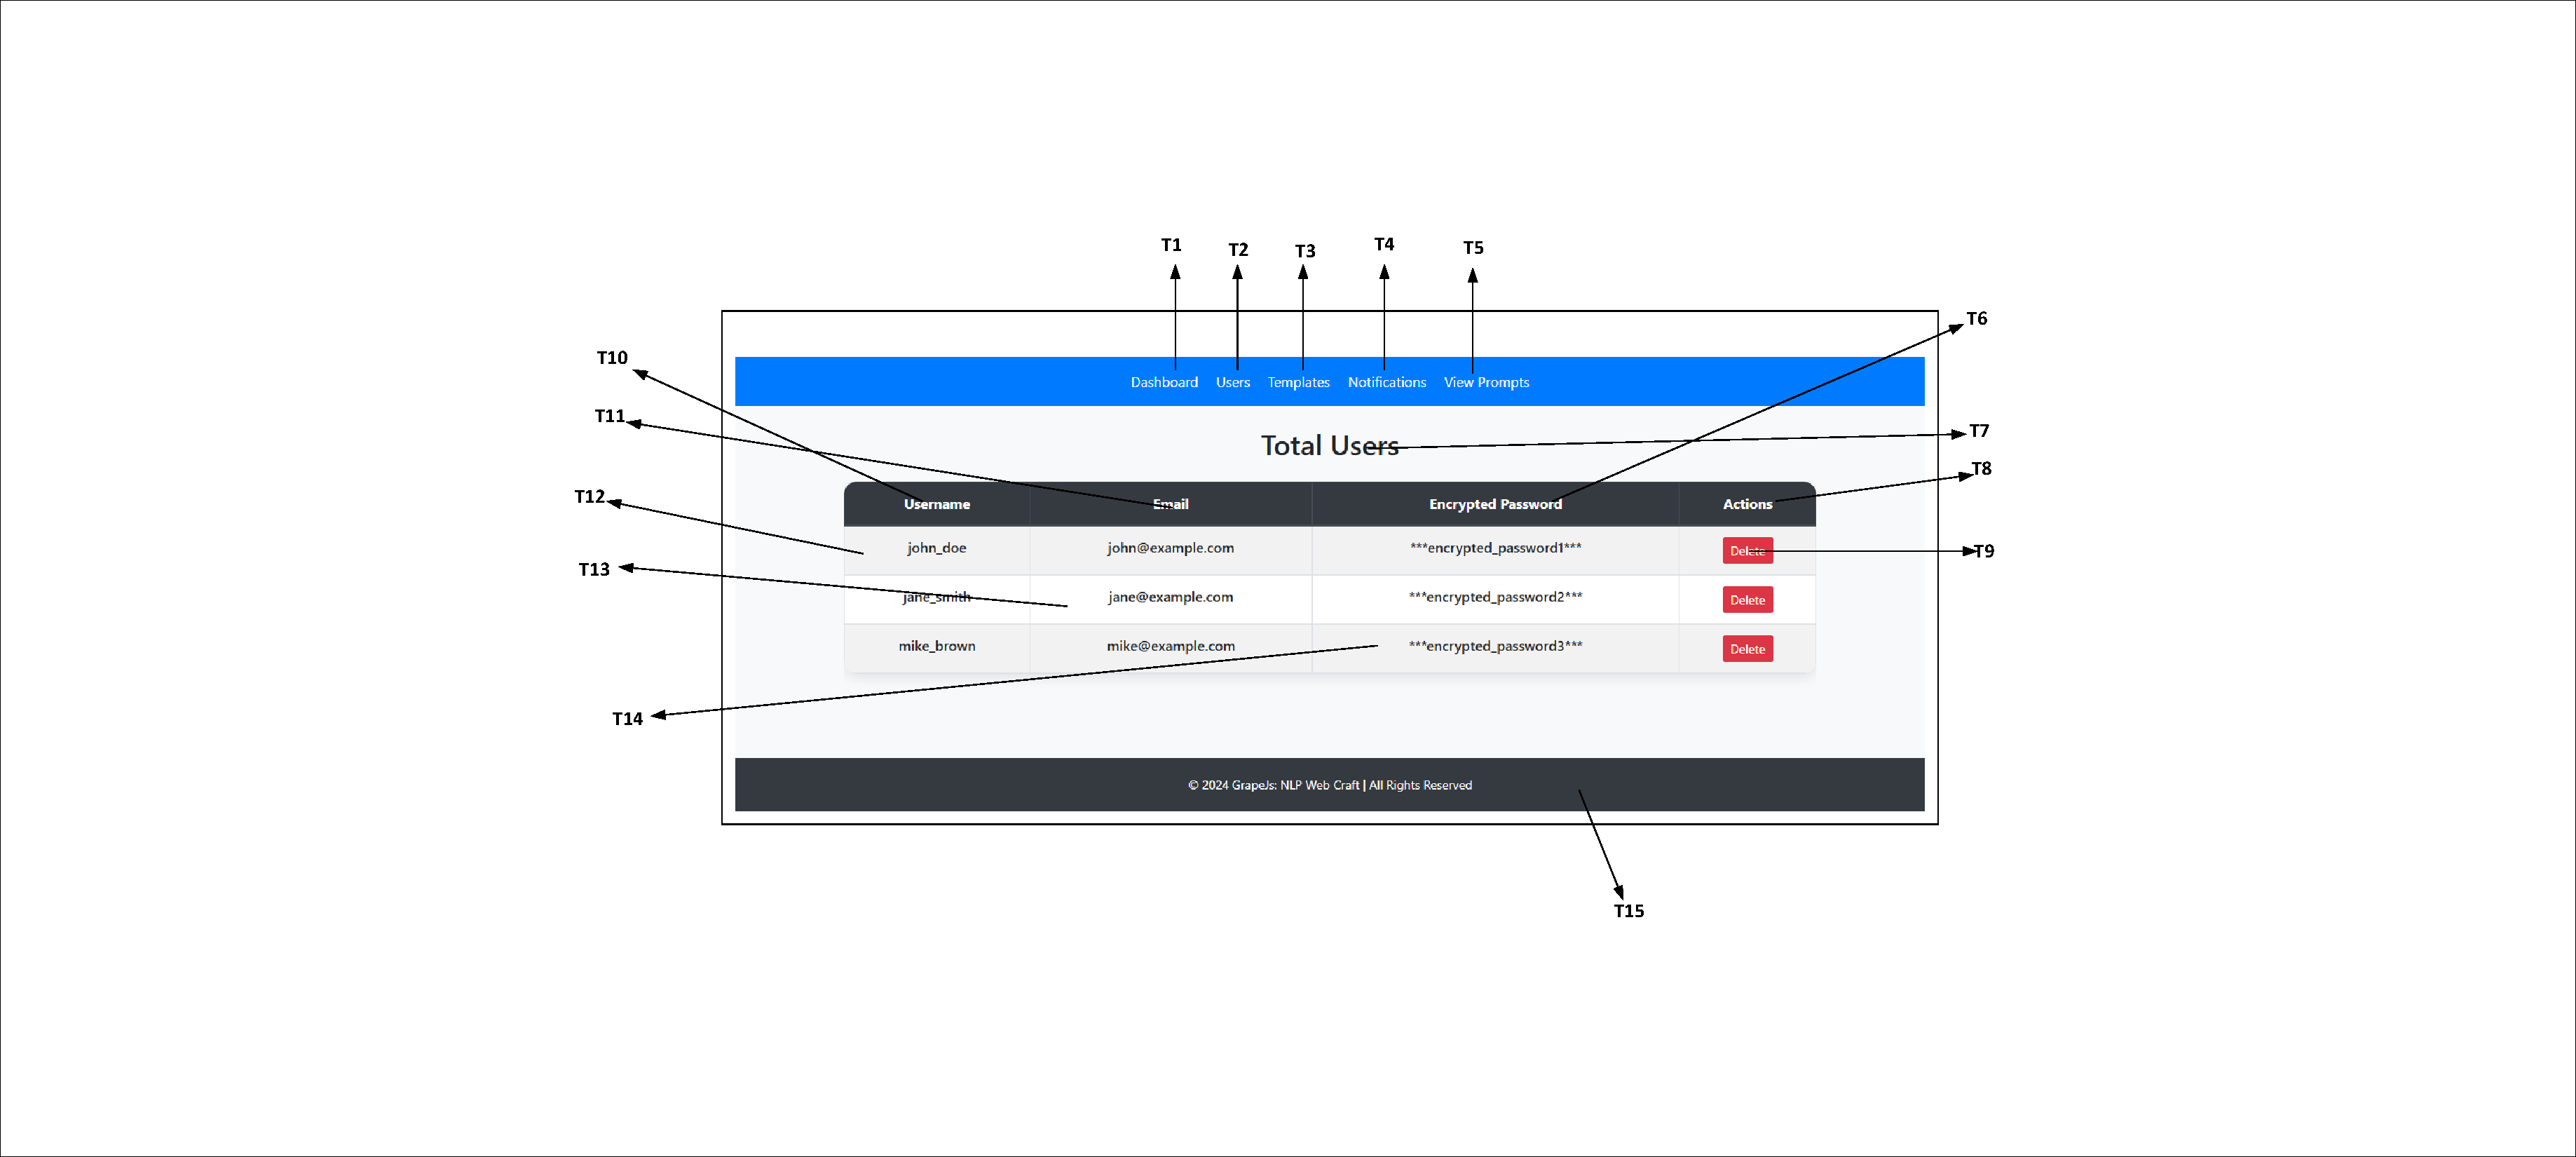
\includegraphics[width=1\textwidth, trim=10cm 5cm 10cm 5cm, clip]{Media/6.pdf} % Path to your image
    \caption{WireFrame: Admin View Users}
    \label{fig:drawing1}
\end{figure}
\begin{table}[h!]
    \centering
    \begin{tabular}{|c|p{10cm}|}
        \hline
        \textbf{Element} & \textbf{Description} \\
        \hline
        T1 & As an admin, I shall click on the dashboard. \\
        \hline
        T2 & As an admin, I shall click on users. \\
        \hline
        T3 & As an admin, I shall click on templates. \\
        \hline
        T4 & As an admin, I shall click on notifications. \\
        \hline
        T5 & As an admin, I shall click on view prompts. \\
        \hline
        T6 & As an admin, I shall view the "Encrypted password" label. \\
        \hline
        T7 & As an admin, I shall view the "Total Users" label. \\
        \hline
        T8 & As an admin, I shall view the "Action" label. \\
        \hline
        T9 & As an admin, I shall click the delete button. \\
        \hline
        T10 & As an admin, I shall view the "Username" label. \\
        \hline
        T11 & As an admin, I shall view the "Email" label. \\
        \hline
        T12 & As an admin, I shall view the username. \\
        \hline
        T13 & As an admin, I shall view the email. \\
        \hline
        T14 & As an admin, I shall view the encrypted password. \\
        \hline
        T15 & As an admin, I shall view the "All rights reserved" label. \\
        \hline
    \end{tabular}
    \caption{WireFrame: Admin View Users}
    \label{tab:admin_user_management_actions}
\end{table}
\begin{figure}[ht]
    \centering
    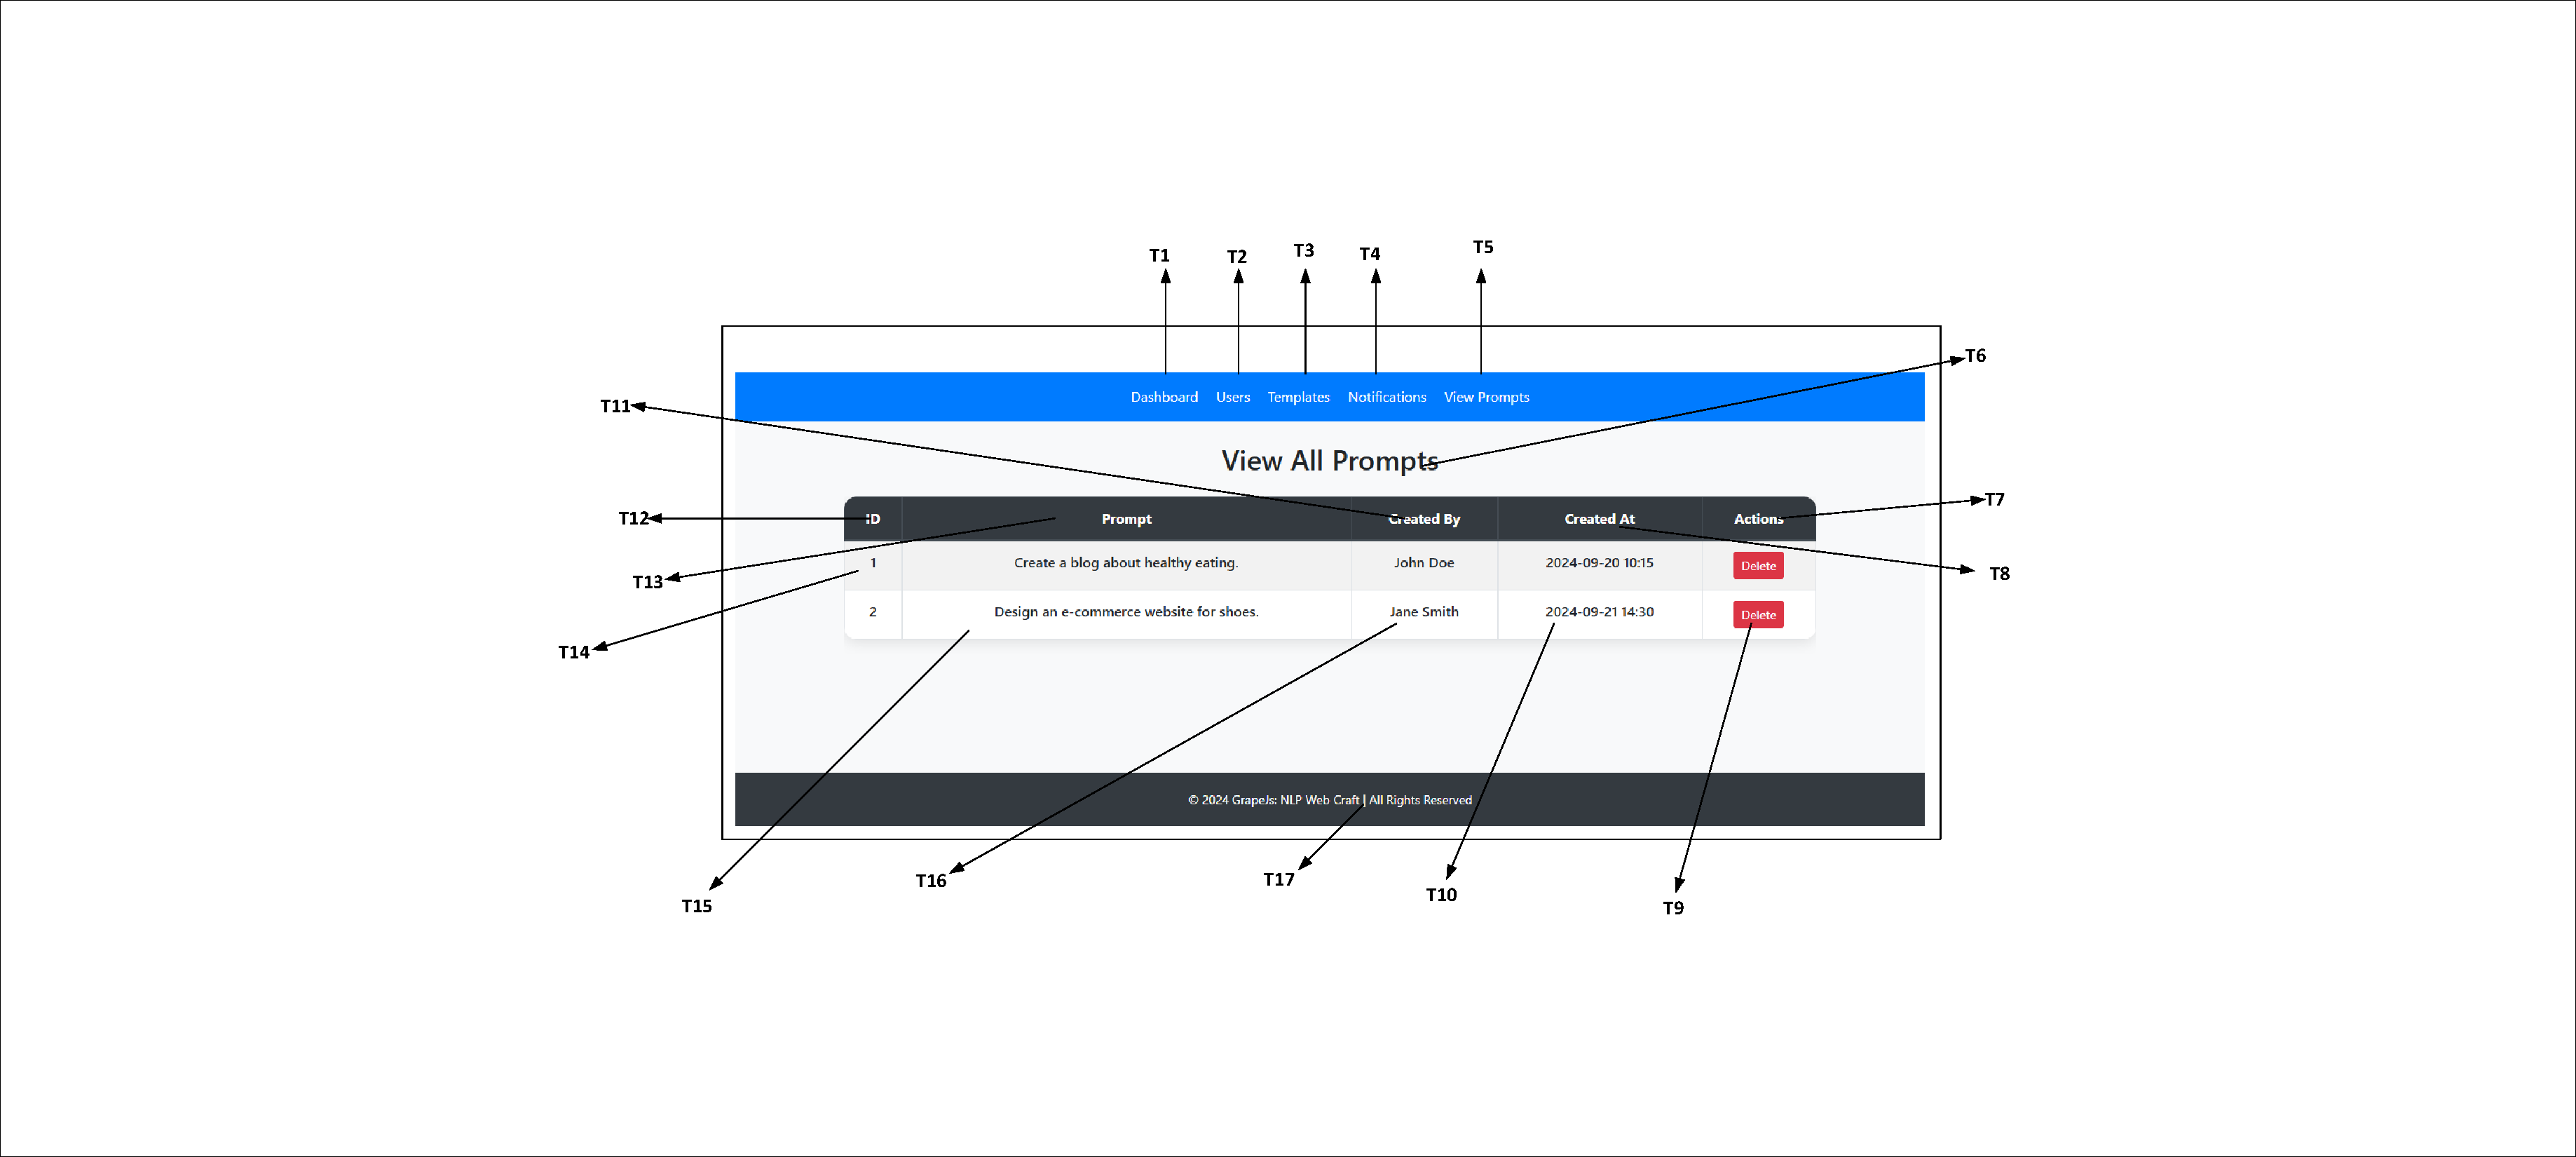
\includegraphics[width=1\textwidth, trim=10cm 5cm 10cm 5cm, clip]{Media/7.pdf} % Path to your PDF
    \caption{WireFrame: Admin View Prompt}
    \label{fig:drawing1}
\end{figure}  



\begin{table}[h!]
    \centering
    \begin{tabular}{|c|p{10cm}|}
        \hline
        \textbf{Element} & \textbf{Description} \\
        \hline
        T1 & As an admin, I shall click on the dashboard. \\
        \hline
        T2 & As an admin, I shall click on users. \\
        \hline
        T3 & As an admin, I shall click on templates. \\
        \hline
        T4 & As an admin, I shall click on notifications. \\
        \hline
        T5 & As an admin, I shall click on view prompts. \\
        \hline
        T6 & As an admin, I shall view the "All prompts" label. \\
        \hline
        T7 & As an admin, I shall view the "Action" label. \\
        \hline
        T8 & As an admin, I shall view the "Created At" label. \\
        \hline
        T9 & As an admin, I shall click the delete button. \\
        \hline
        T10 & As an admin, I shall view "Created At." \\
        \hline
        T11 & As an admin, I shall view the "Created By" label. \\
        \hline
        T12 & As an admin, I shall view the "ID" label. \\
        \hline
        T13 & As an admin, I shall view the "Prompt" label. \\
        \hline
        T14 & As an admin, I shall view the ID number. \\
        \hline
        T15 & As an admin, I shall view the prompt. \\
        \hline
        T16 & As an admin, I shall view the "Created By" name. \\
        \hline
        T17 & As an admin, I shall view the "All rights reserved" label. \\
        \hline
    \end{tabular}
    \caption{WireFrame: Admin View Prompt}
    \label{tab:admin_prompt_management_actions}
\end{table}


\clearpage
\section{System Behavioral Design}
\subsection{Activity Diagram}

\begin{figure}[ht]
    \centering
    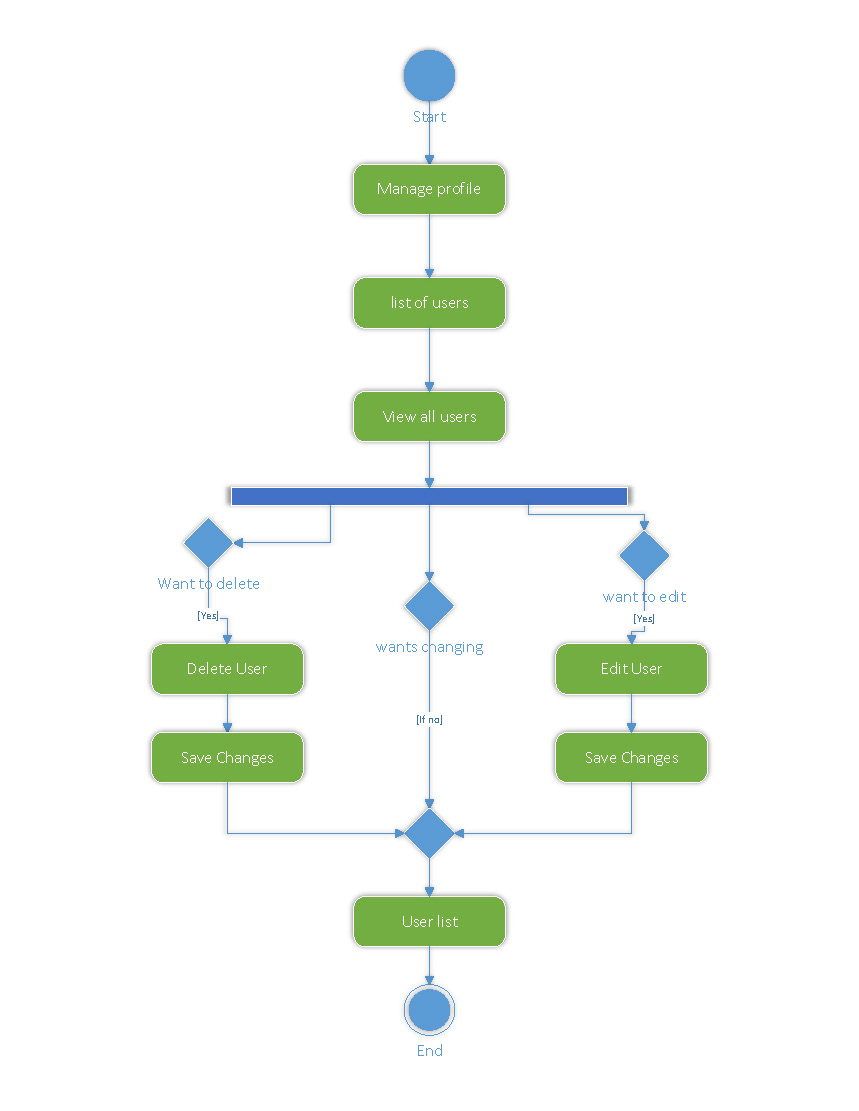
\includegraphics[width=0.8\textwidth]{Media/Binder2.pdf_Page_01.jpg} % Path to your image
    \caption{Activity Diagram: Manage User Profile (Admin)}
    \label{fig:drawing1}
\end{figure}

\begin{figure}[ht]
    \centering
    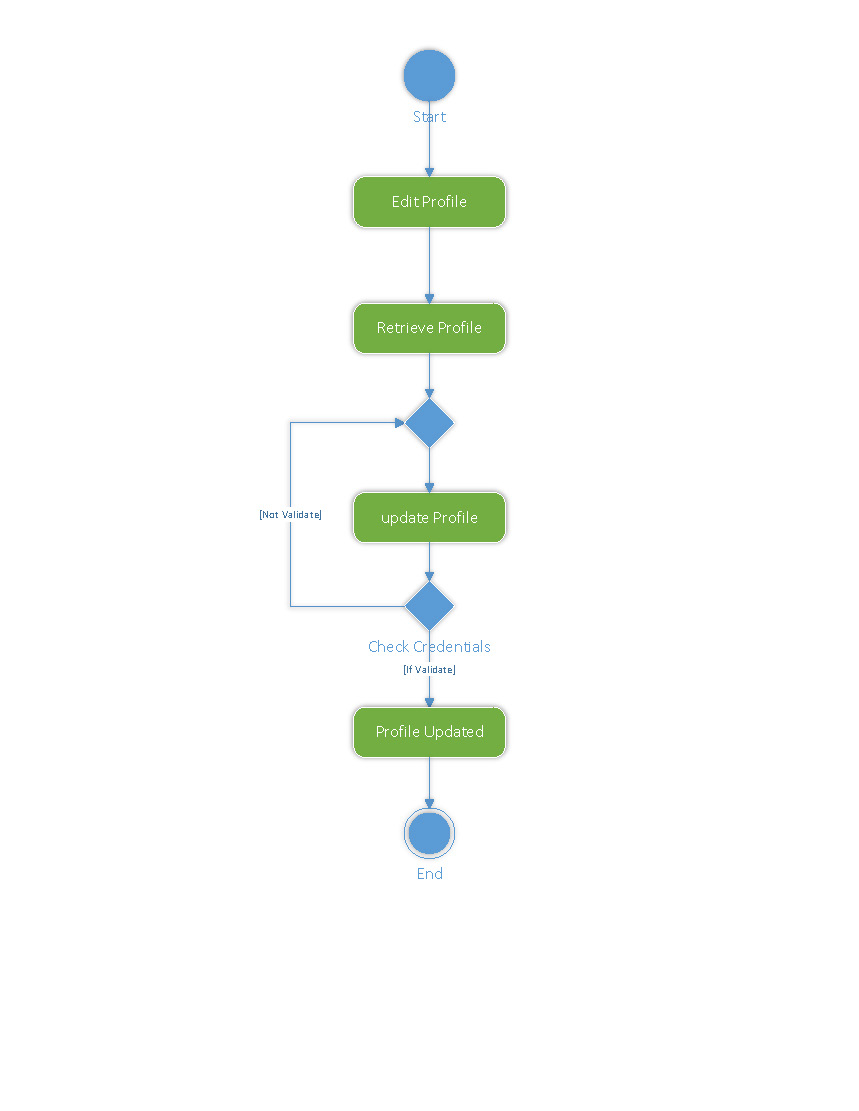
\includegraphics[width=0.8\textwidth]{Media/Binder2.pdf_Page_02.jpg} % Path to your image
    \caption{Activity Diagram: Edit Profile (Admin)}
    \label{fig:drawing1}
\end{figure}

\begin{figure}[ht]
    \centering
    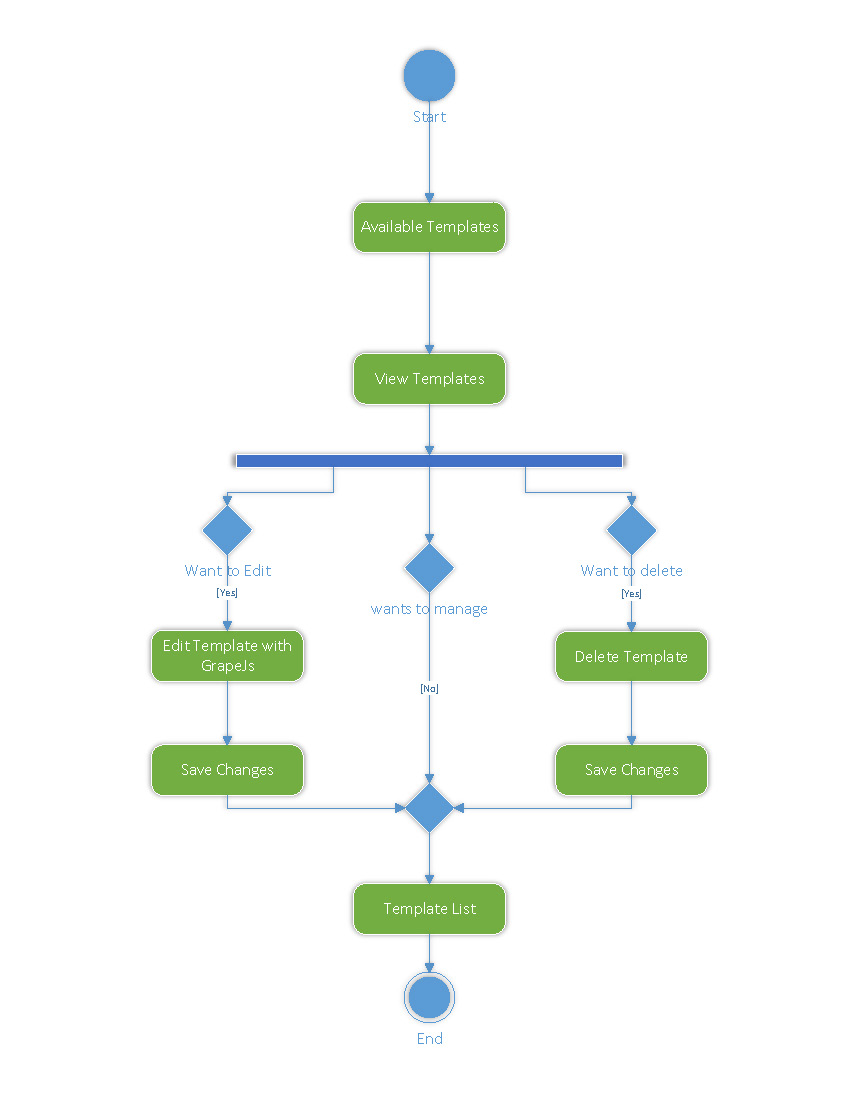
\includegraphics[width=0.8\textwidth]{Media/Binder2.pdf_Page_03.jpg} % Path to your image
    \caption{Activity Diagram: Manage Templates (Admin)}
    \label{fig:drawing1}
\end{figure}

\begin{figure}[ht]
    \centering
    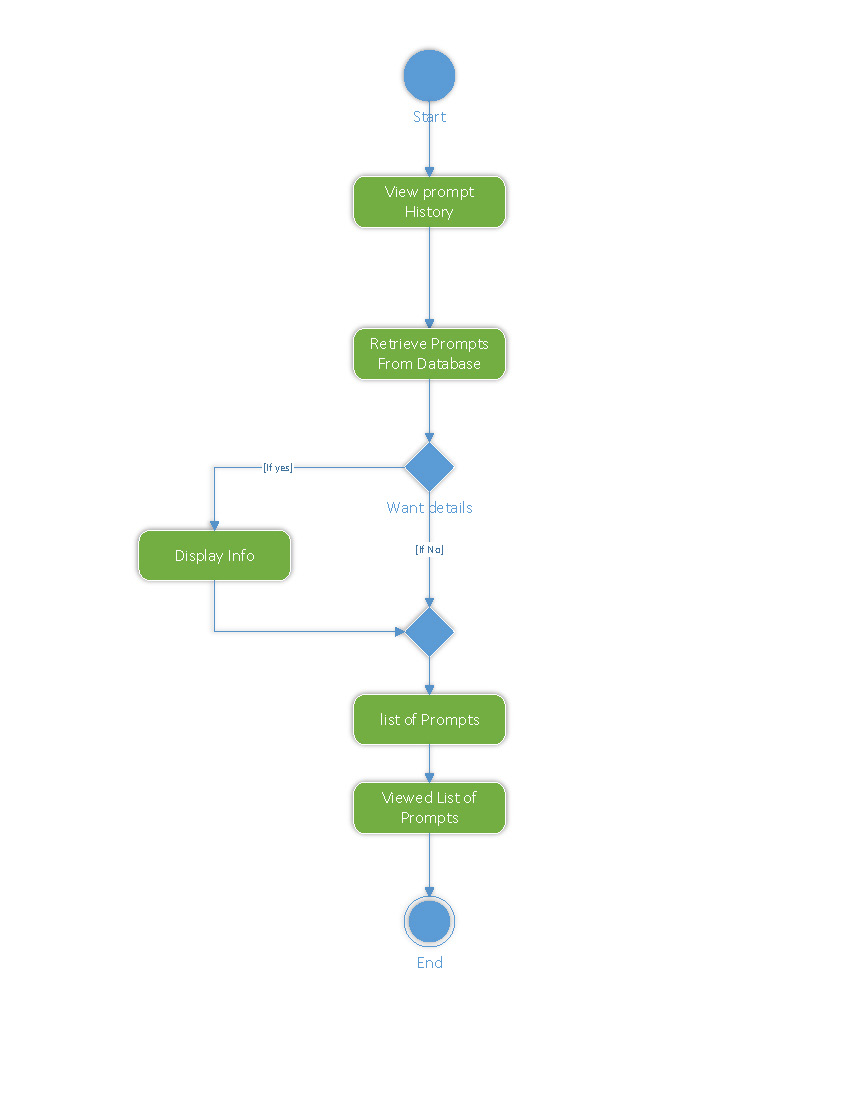
\includegraphics[width=0.8\textwidth]{Media/Binder2.pdf_Page_04.jpg} % Path to your image
    \caption{Activity Diagram: View Prompt History (Admin)}
    \label{fig:drawing1}
\end{figure}

\begin{figure}[ht]
    \centering
    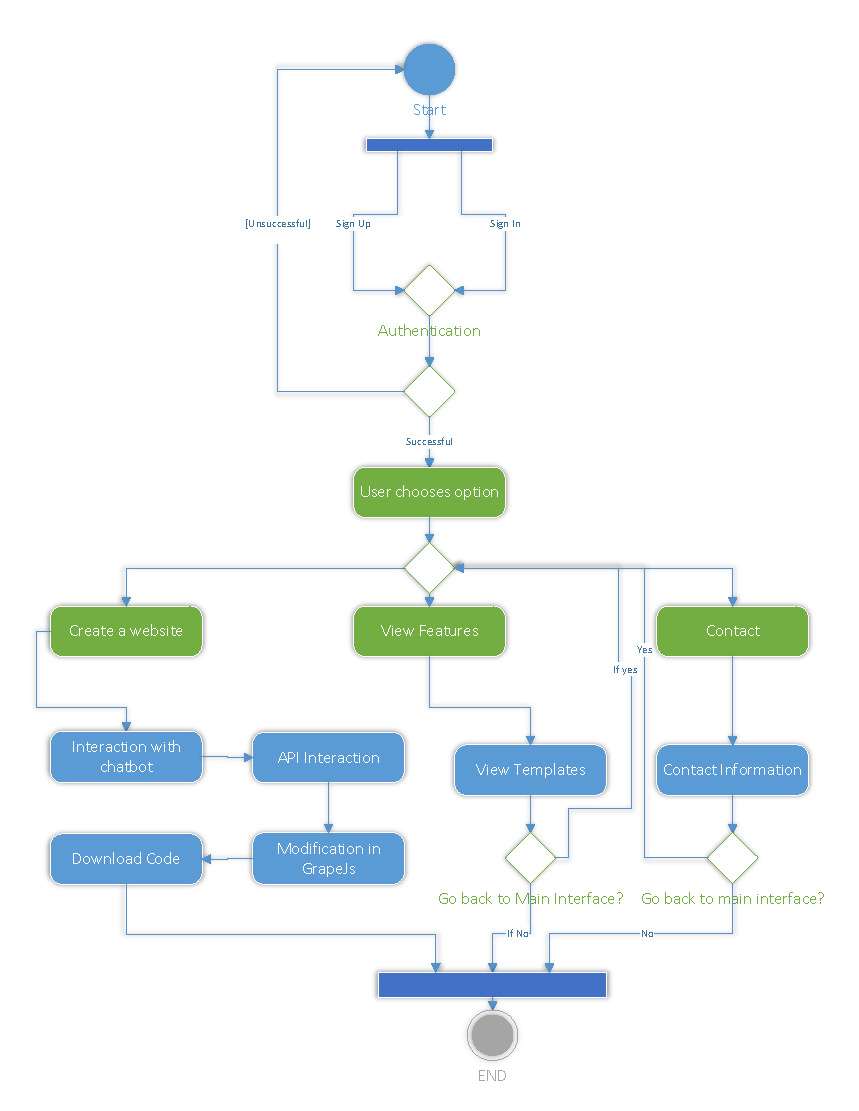
\includegraphics[width=0.8\textwidth]{Media/Binder2.pdf_Page_05.jpg} % Path to your image
    \caption{Activity Diagram: Web Creation Process (User)}
    \label{fig:drawing1}
\end{figure}

\begin{figure}[ht]
    \centering
    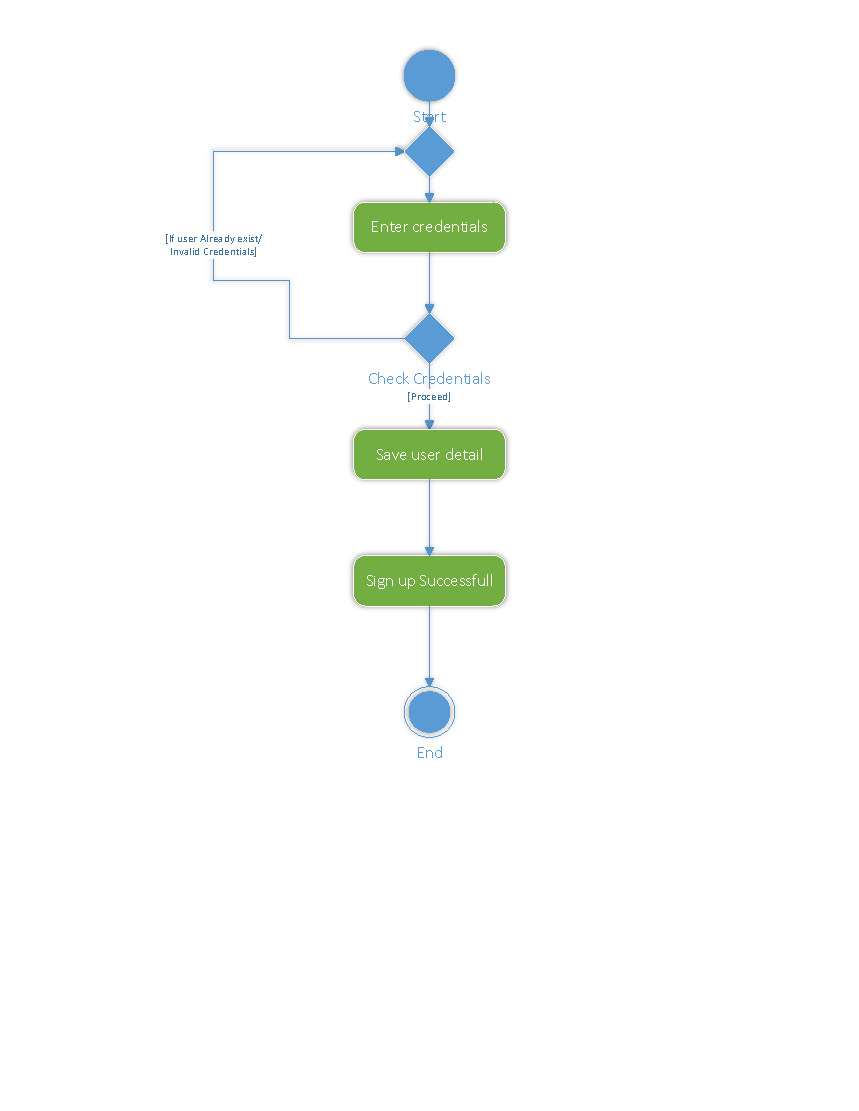
\includegraphics[width=0.8\textwidth]{Media/Binder2.pdf_Page_06.jpg} % Path to your image
    \caption{Activity Diagram: Sign Up (User/Admin)}
    \label{fig:drawing1}
\end{figure}

\begin{figure}[ht]
    \centering
    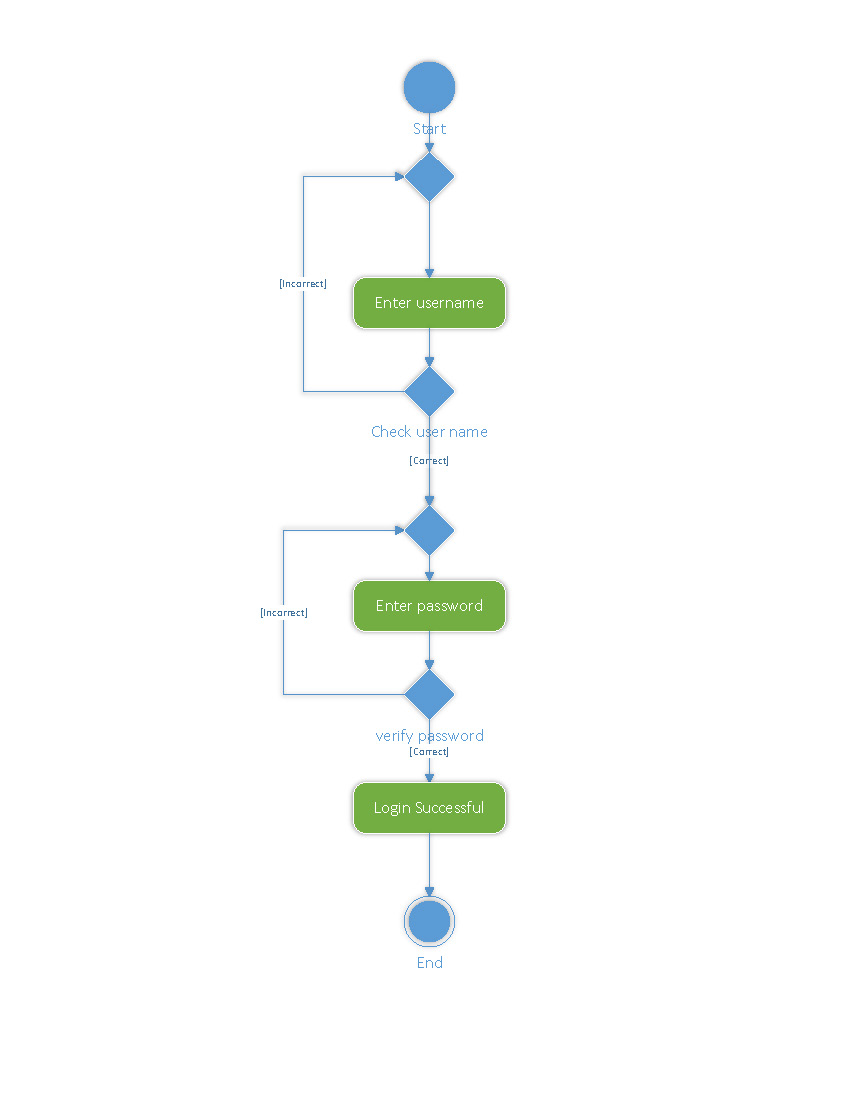
\includegraphics[width=0.8\textwidth]{Media/Binder2.pdf_Page_07.jpg} % Path to your image
    \caption{Activity Diagram: Sign In (User/Admin)}
    \label{fig:drawing1}
\end{figure}

\begin{figure}[ht]
    \centering
    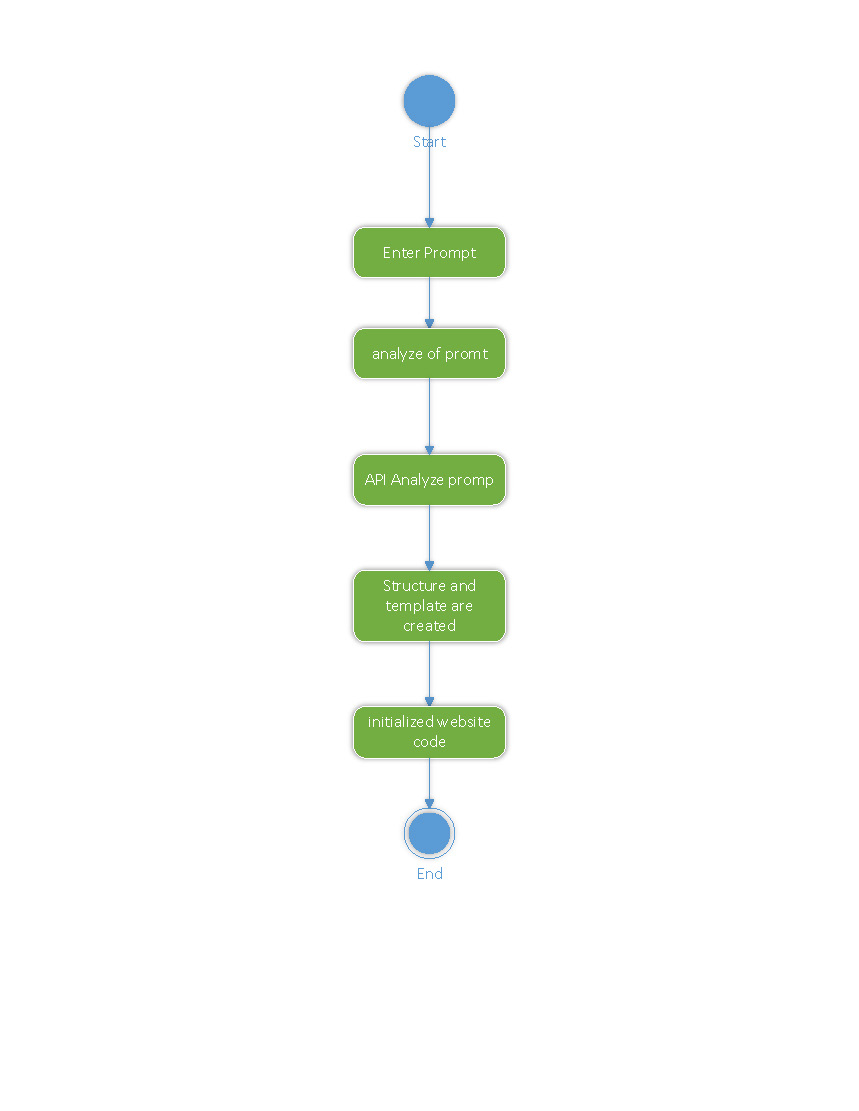
\includegraphics[width=0.8\textwidth]{Media/Binder2.pdf_Page_08.jpg} % Path to your image
    \caption{Activity Diagram: Rendering of Prompt (User)}
    \label{fig:drawing1}
\end{figure}

\begin{figure}[ht]
    \centering
    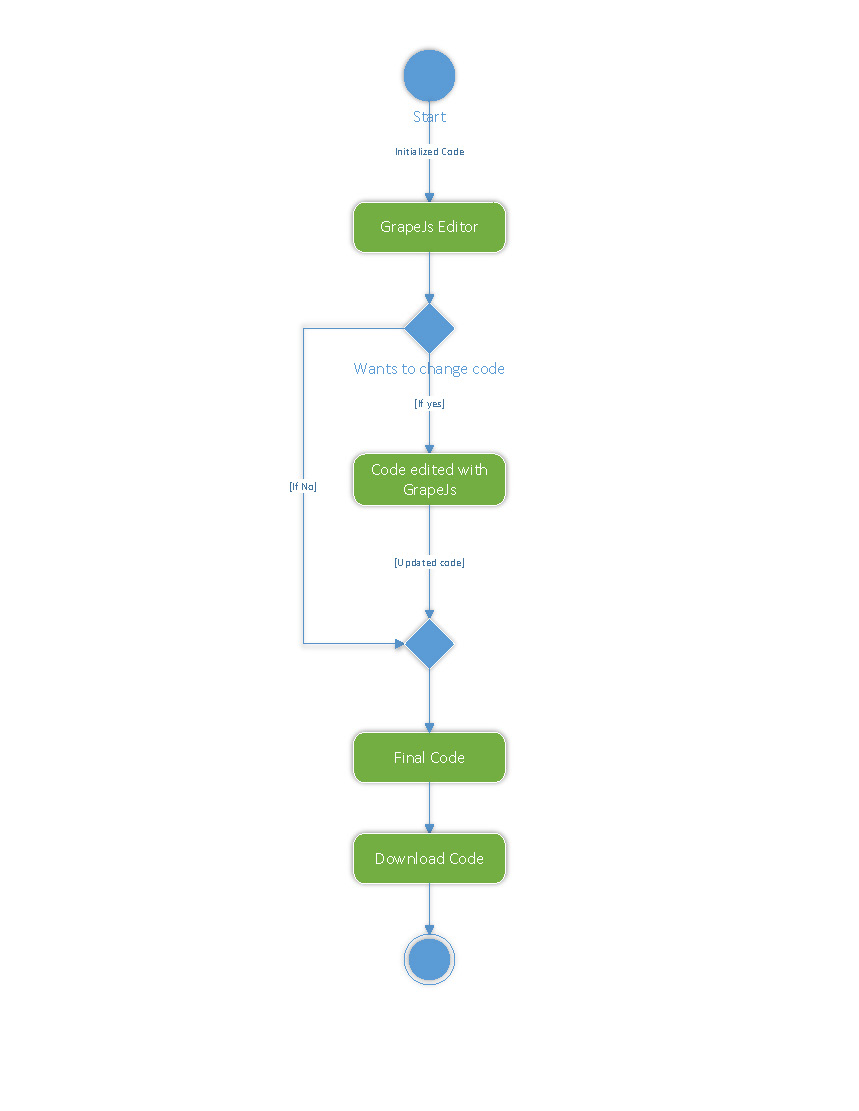
\includegraphics[width=0.8\textwidth]{Media/Binder2.pdf_Page_09.jpg} % Path to your image
    \caption{Activity Diagram: Editing With Grapejs (User)}
    \label{fig:drawing1}
\end{figure}

\begin{figure}[ht]
    \centering
    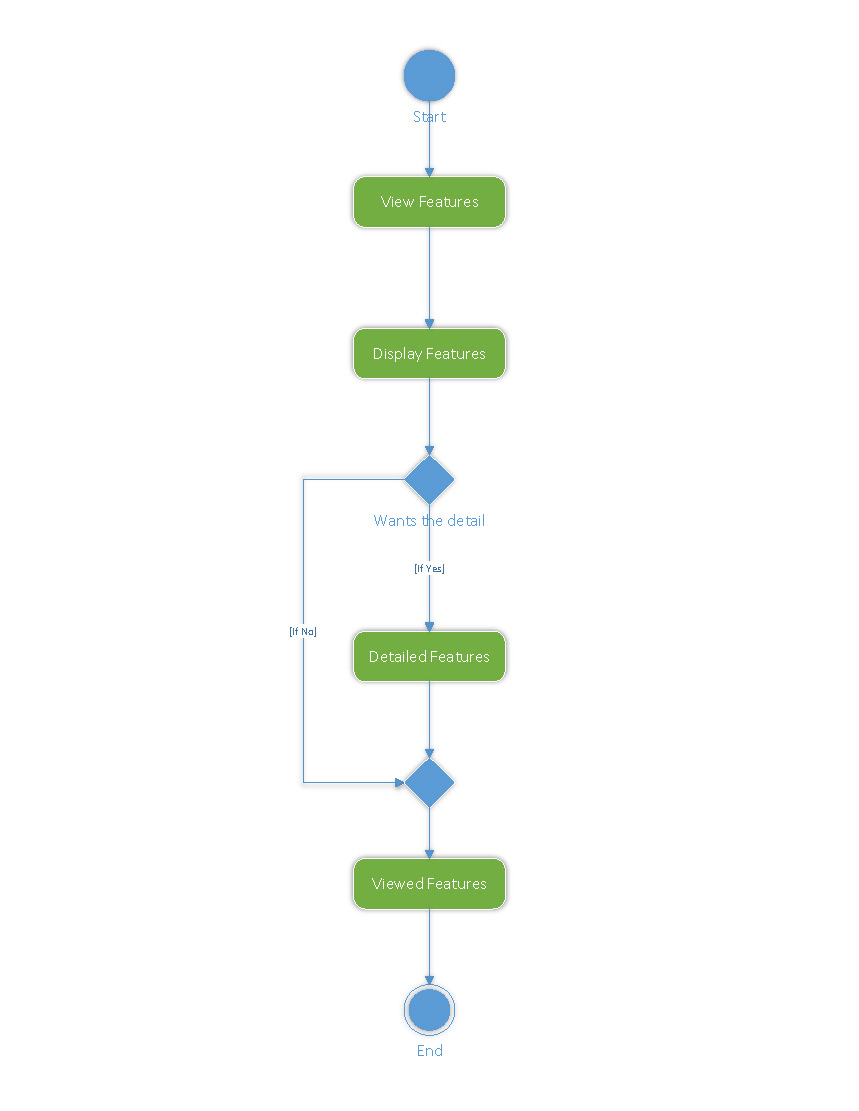
\includegraphics[width=0.8\textwidth]{Media/Binder2.pdf_Page_10.jpg} % Path to your image
    \caption{Activity Diagram: Feature View (User)}
    \label{fig:drawing1}
\end{figure}

\begin{figure}[ht]
    \centering
    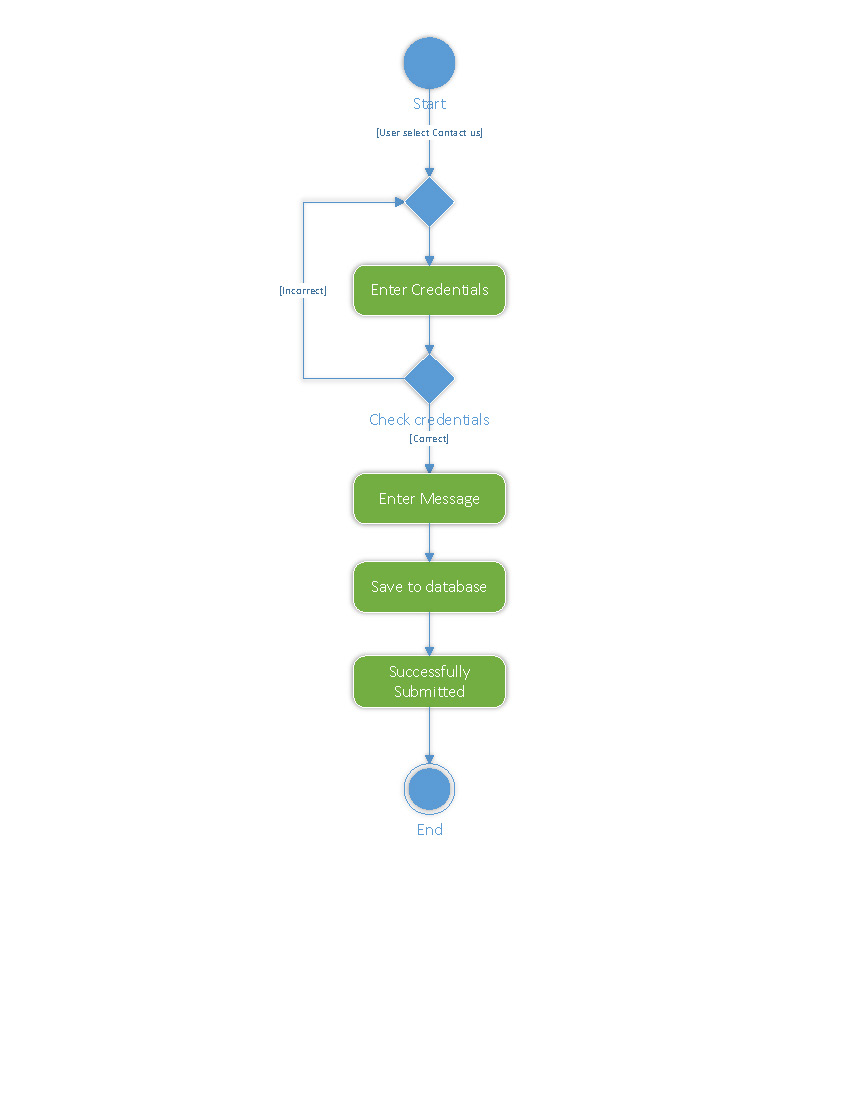
\includegraphics[width=0.8\textwidth]{Media/Binder2.pdf_Page_11.jpg} % Path to your image
    \caption{Activity Diagram: Contact (User)}
    \label{fig:drawing1}
\end{figure}







\clearpage   % Remaining
\subsection{State Diagram}

\begin{figure}[ht]
    \centering
    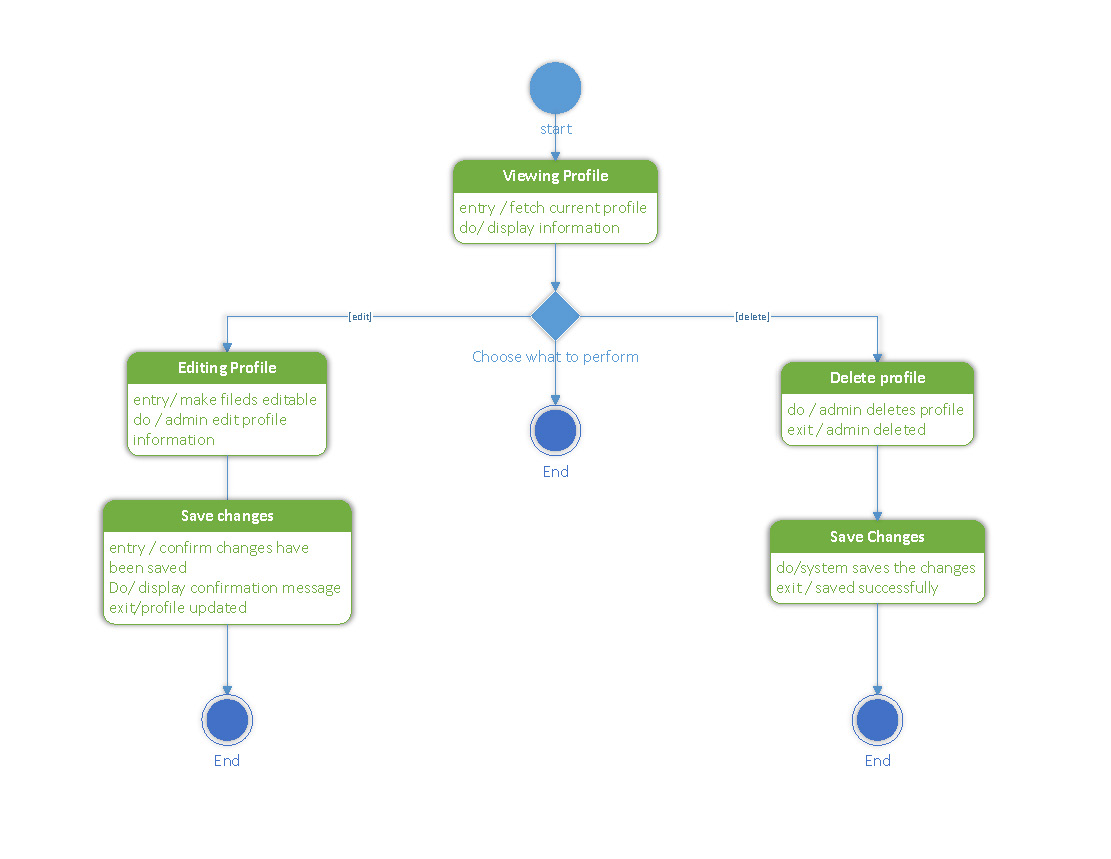
\includegraphics[width=0.8\textwidth]{Media/Binder2.pdf_Page_12.jpg} % Path to your image
    \caption{State Diagram: Manage User Profile (Admin)}
    \label{fig:drawing1}
\end{figure}

\begin{figure}[ht]
    \centering
    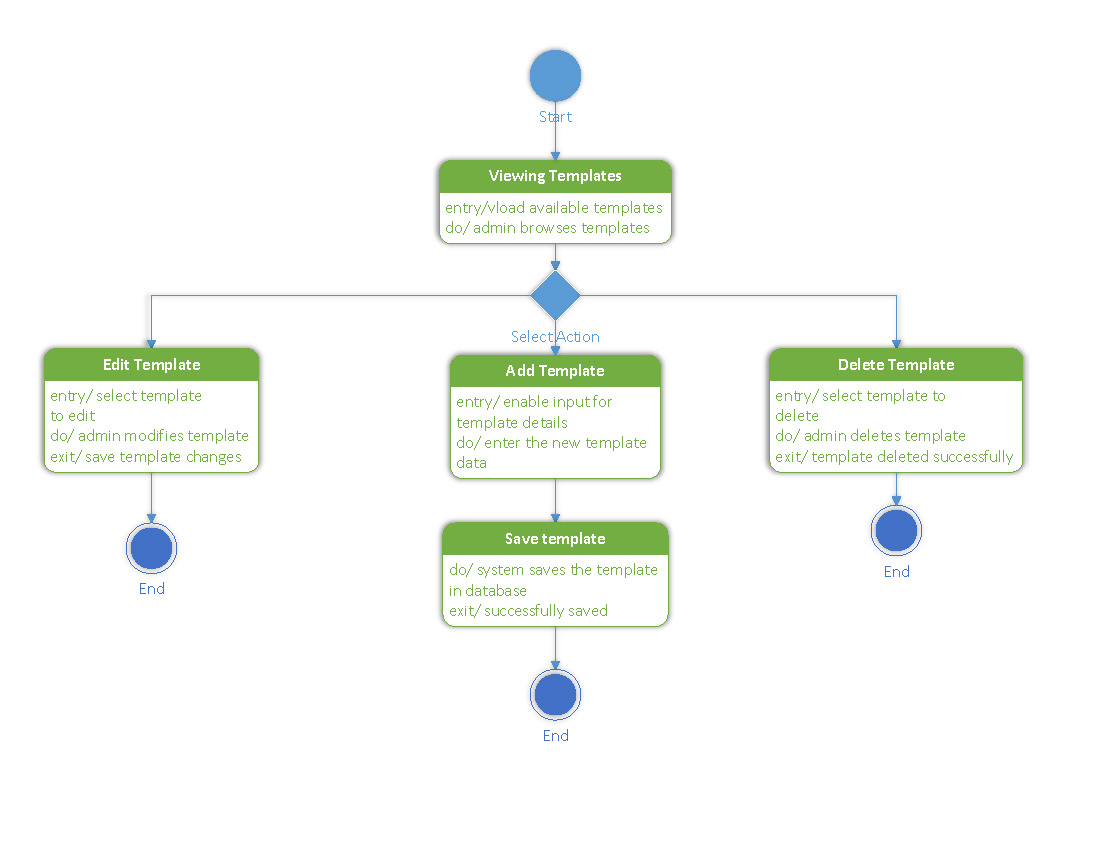
\includegraphics[width=0.8\textwidth]{Media/Binder2.pdf_Page_13.jpg} % Path to your image
    \caption{State Diagram: Manage Templates (Admin)}
    \label{fig:drawing1}
\end{figure}

\begin{figure}[ht]
    \centering
    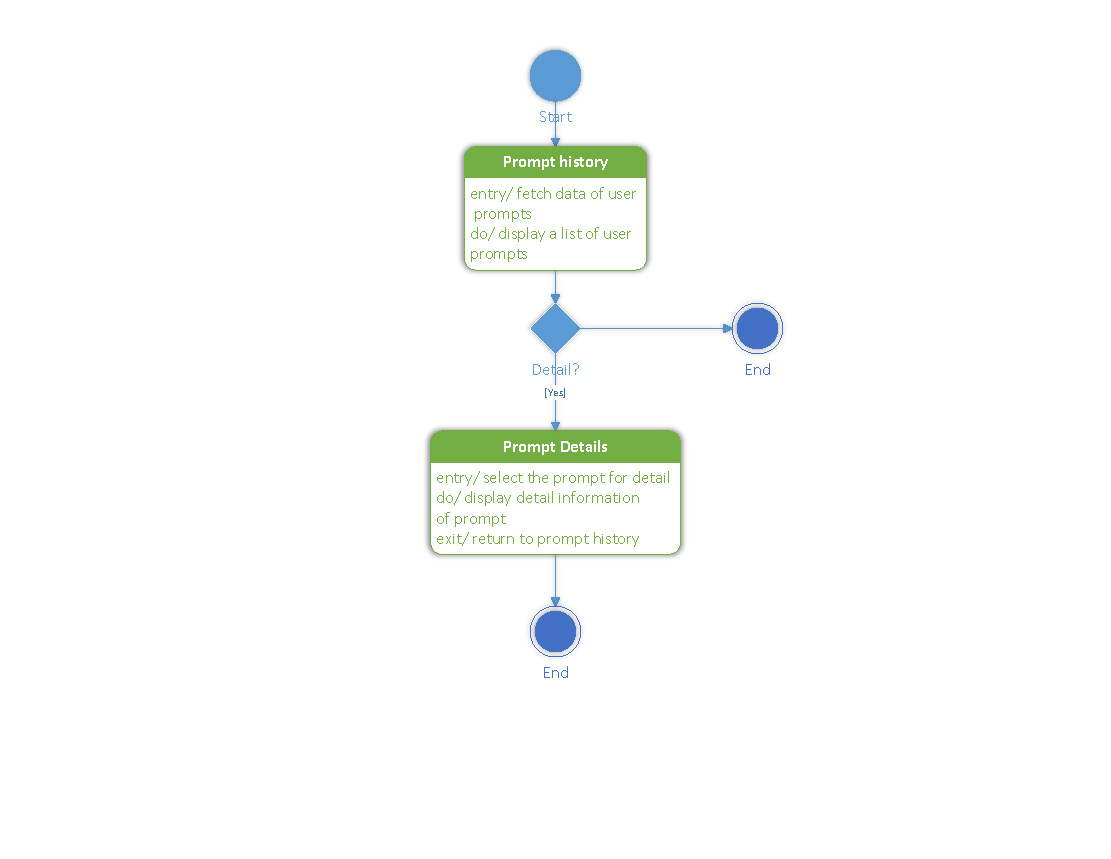
\includegraphics[width=0.8\textwidth]{Media/Binder2.pdf_Page_14.jpg} % Path to your image
    \caption{State Diagram: View Prompt History (Admin)}
    \label{fig:drawing1}
\end{figure}

\begin{figure}[ht]
    \centering
    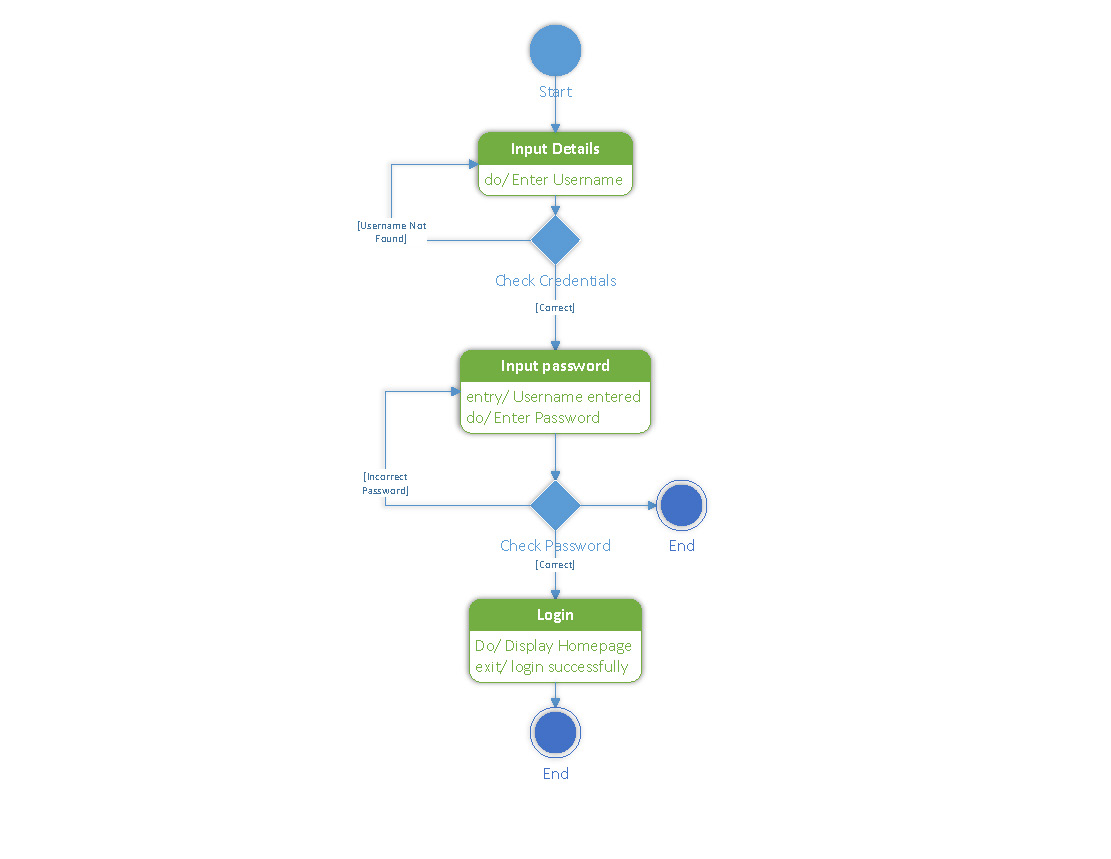
\includegraphics[width=0.8\textwidth]{Media/Binder2.pdf_Page_15.jpg} % Path to your image
    \caption{State Diagram: SignUp (Admin/User)}
    \label{fig:drawing1}
\end{figure}

\begin{figure}[ht]
    \centering
    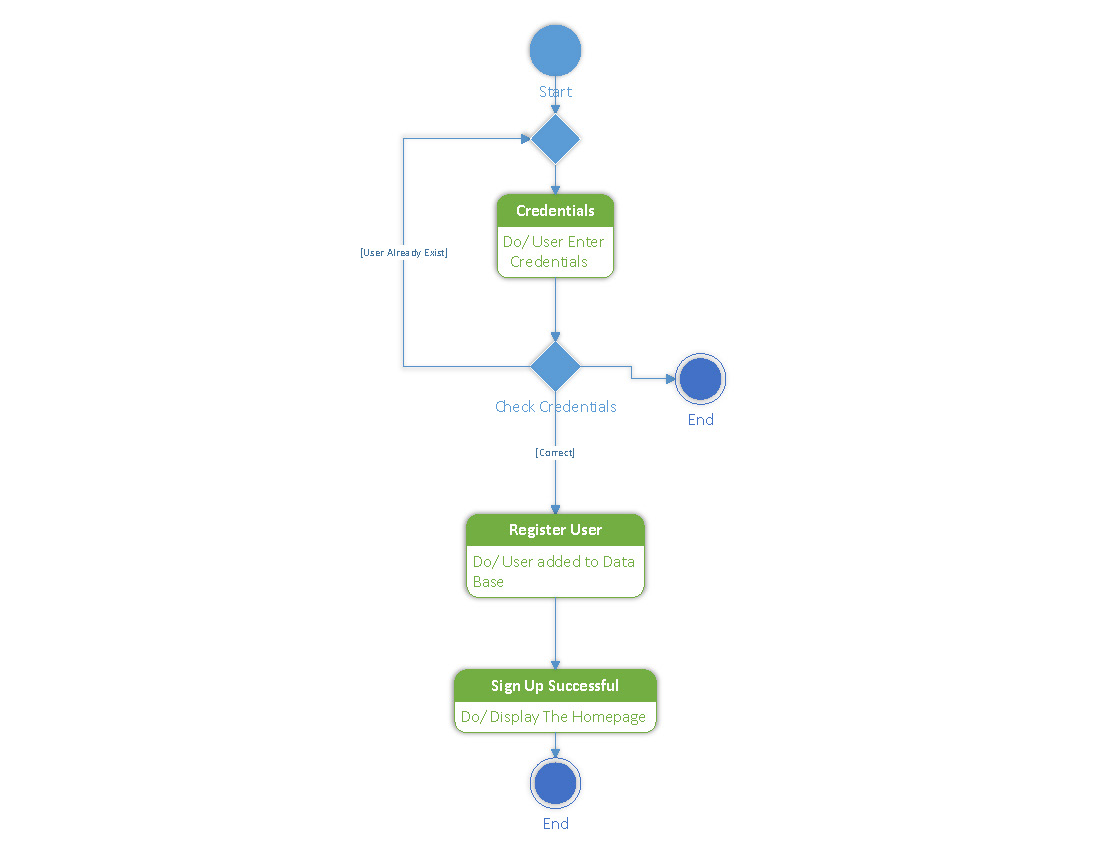
\includegraphics[width=0.8\textwidth]{Media/Binder2.pdf_Page_16.jpg} % Path to your image
    \caption{State Diagram: SignIn (Admin/User)}
    \label{fig:drawing1}
\end{figure}

\begin{figure}[ht]
    \centering
    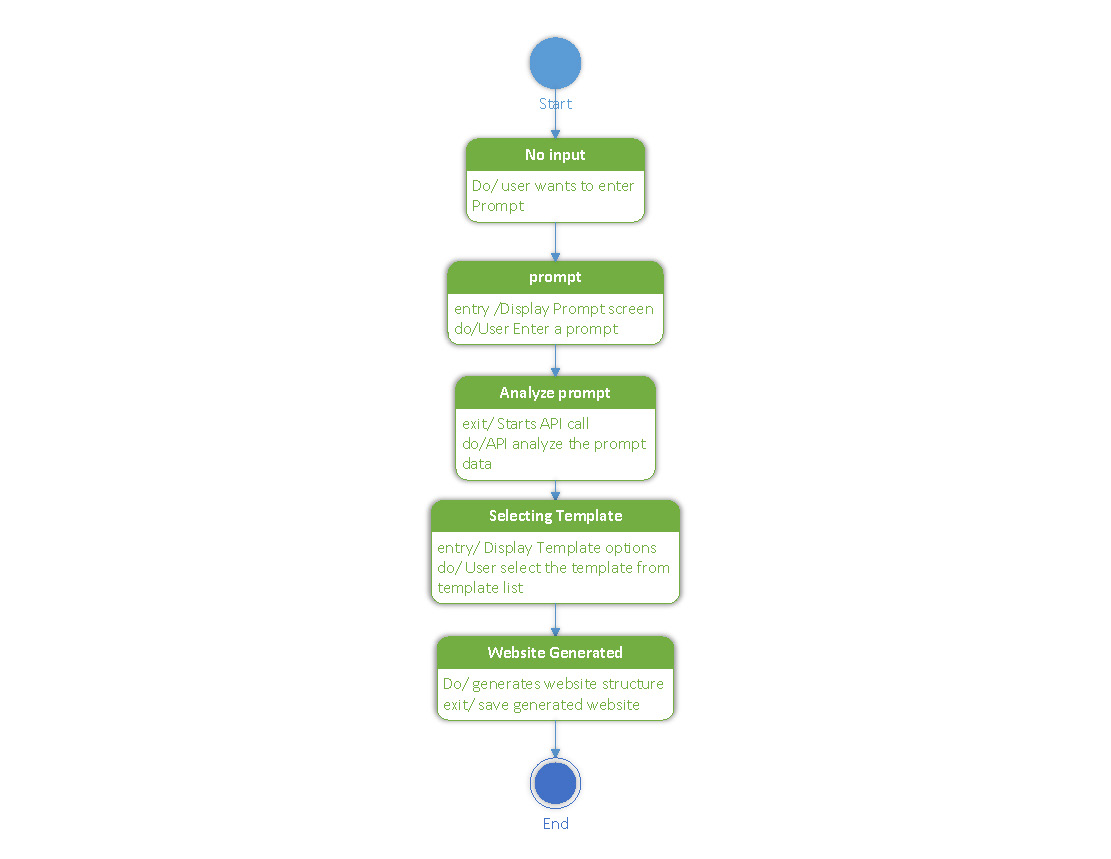
\includegraphics[width=0.8\textwidth]{Media/Binder2.pdf_Page_17.jpg} % Path to your image
    \caption{State Diagram: Rendering of Prompt (User)}
    \label{fig:drawing1}
\end{figure}

\begin{figure}[ht]
    \centering
    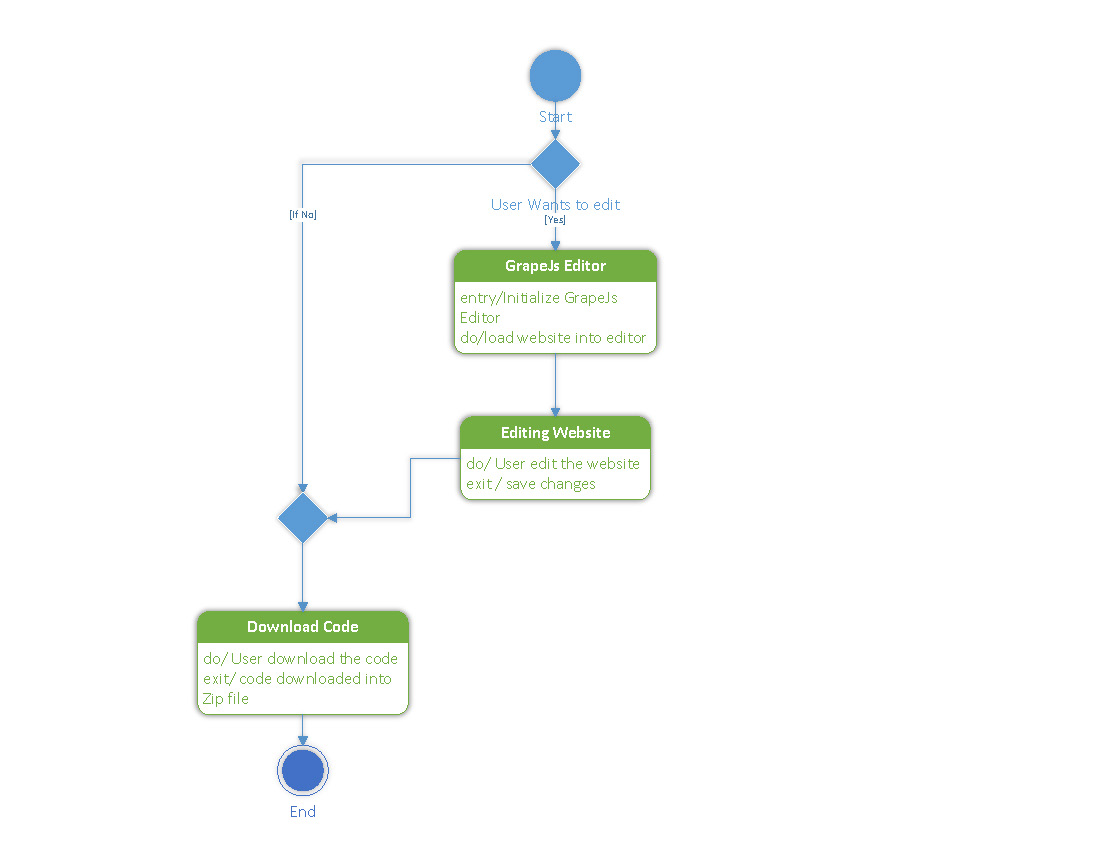
\includegraphics[width=0.8\textwidth]{Media/Binder2.pdf_Page_18.jpg} % Path to your image
    \caption{State Diagram: Download Code (User)}
    \label{fig:drawing1}
\end{figure}

\begin{figure}[ht]
    \centering
    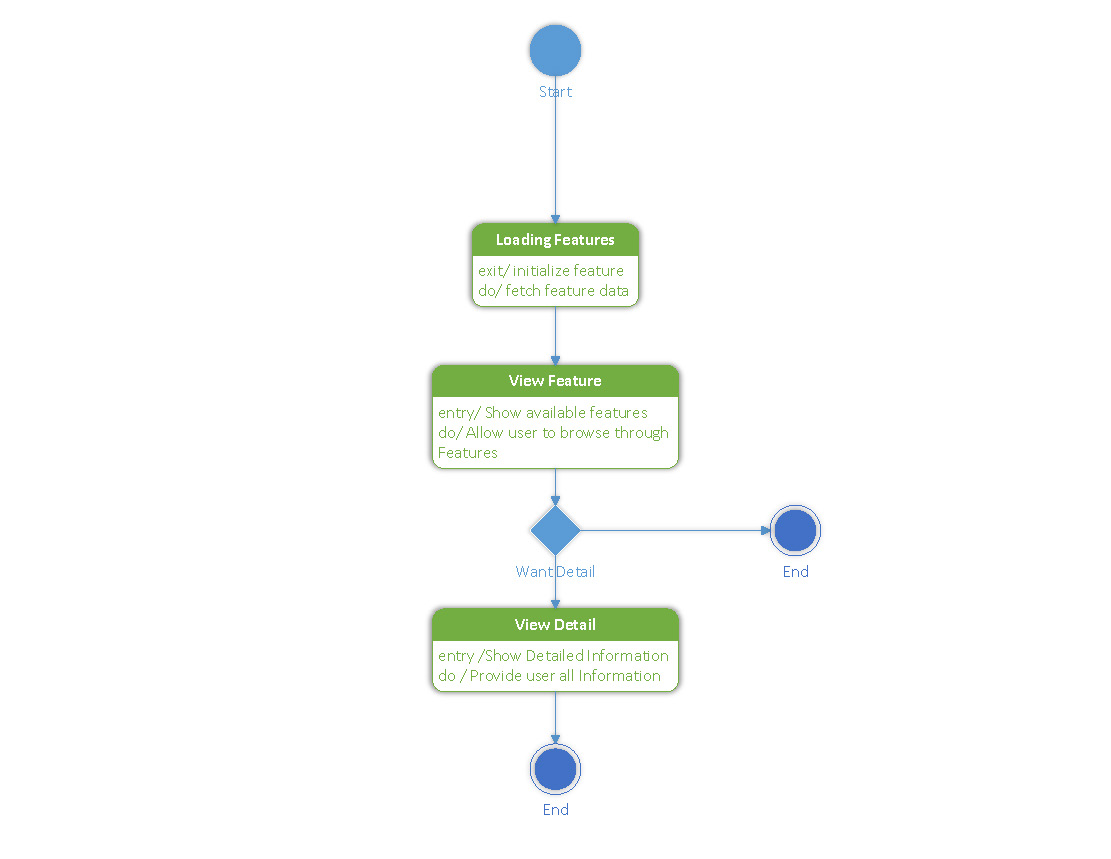
\includegraphics[width=0.8\textwidth]{Media/Binder2.pdf_Page_19.jpg} % Path to your image
    \caption{State Diagram: Editing with GrapeJS (User)}
    \label{fig:drawing1}
\end{figure}

\begin{figure}[ht]
    \centering
    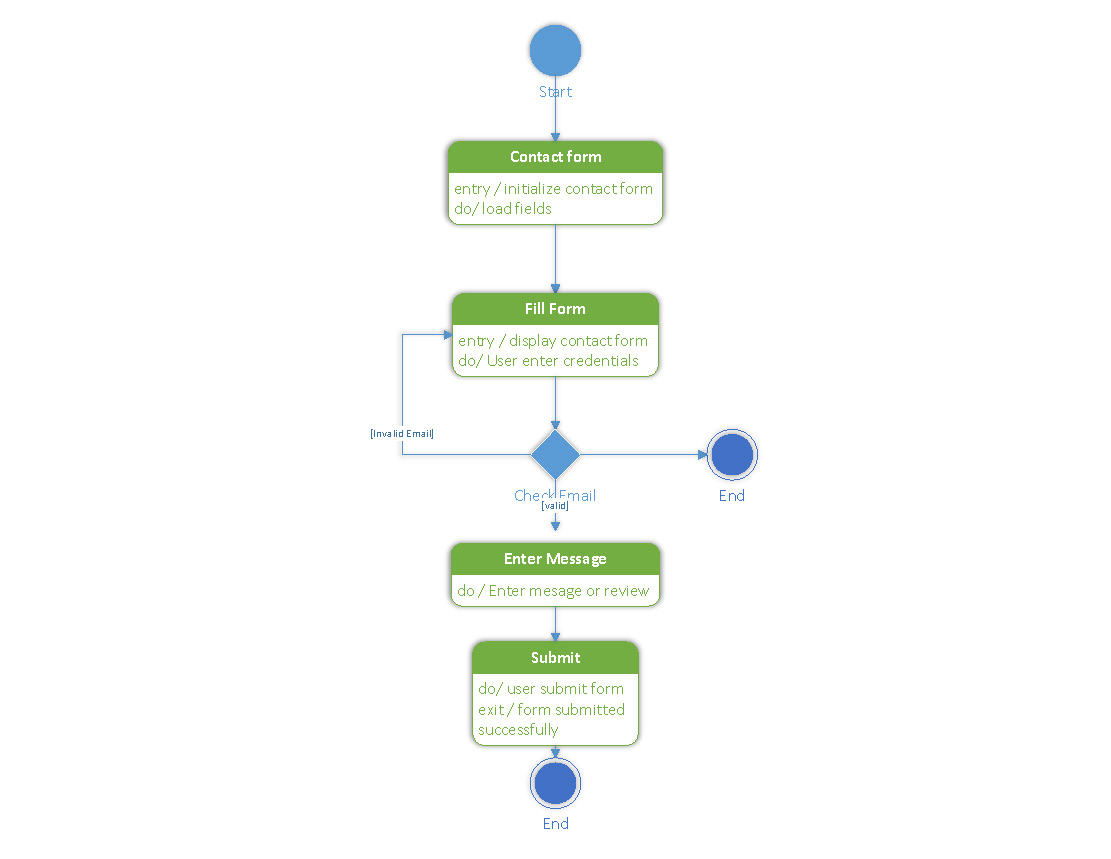
\includegraphics[width=0.8\textwidth]{Media/Binder2.pdf_Page_20.jpg} % Path to your image
    \caption{State Diagram: Contact (User)}
    \label{fig:drawing1}
\end{figure}

\clearpage
       % Remaining
\subsection{Sequence Diagrams}
The following sequence diagrams illustrate the interactions within the system. 

\begin{figure}[ht]
    \centering
    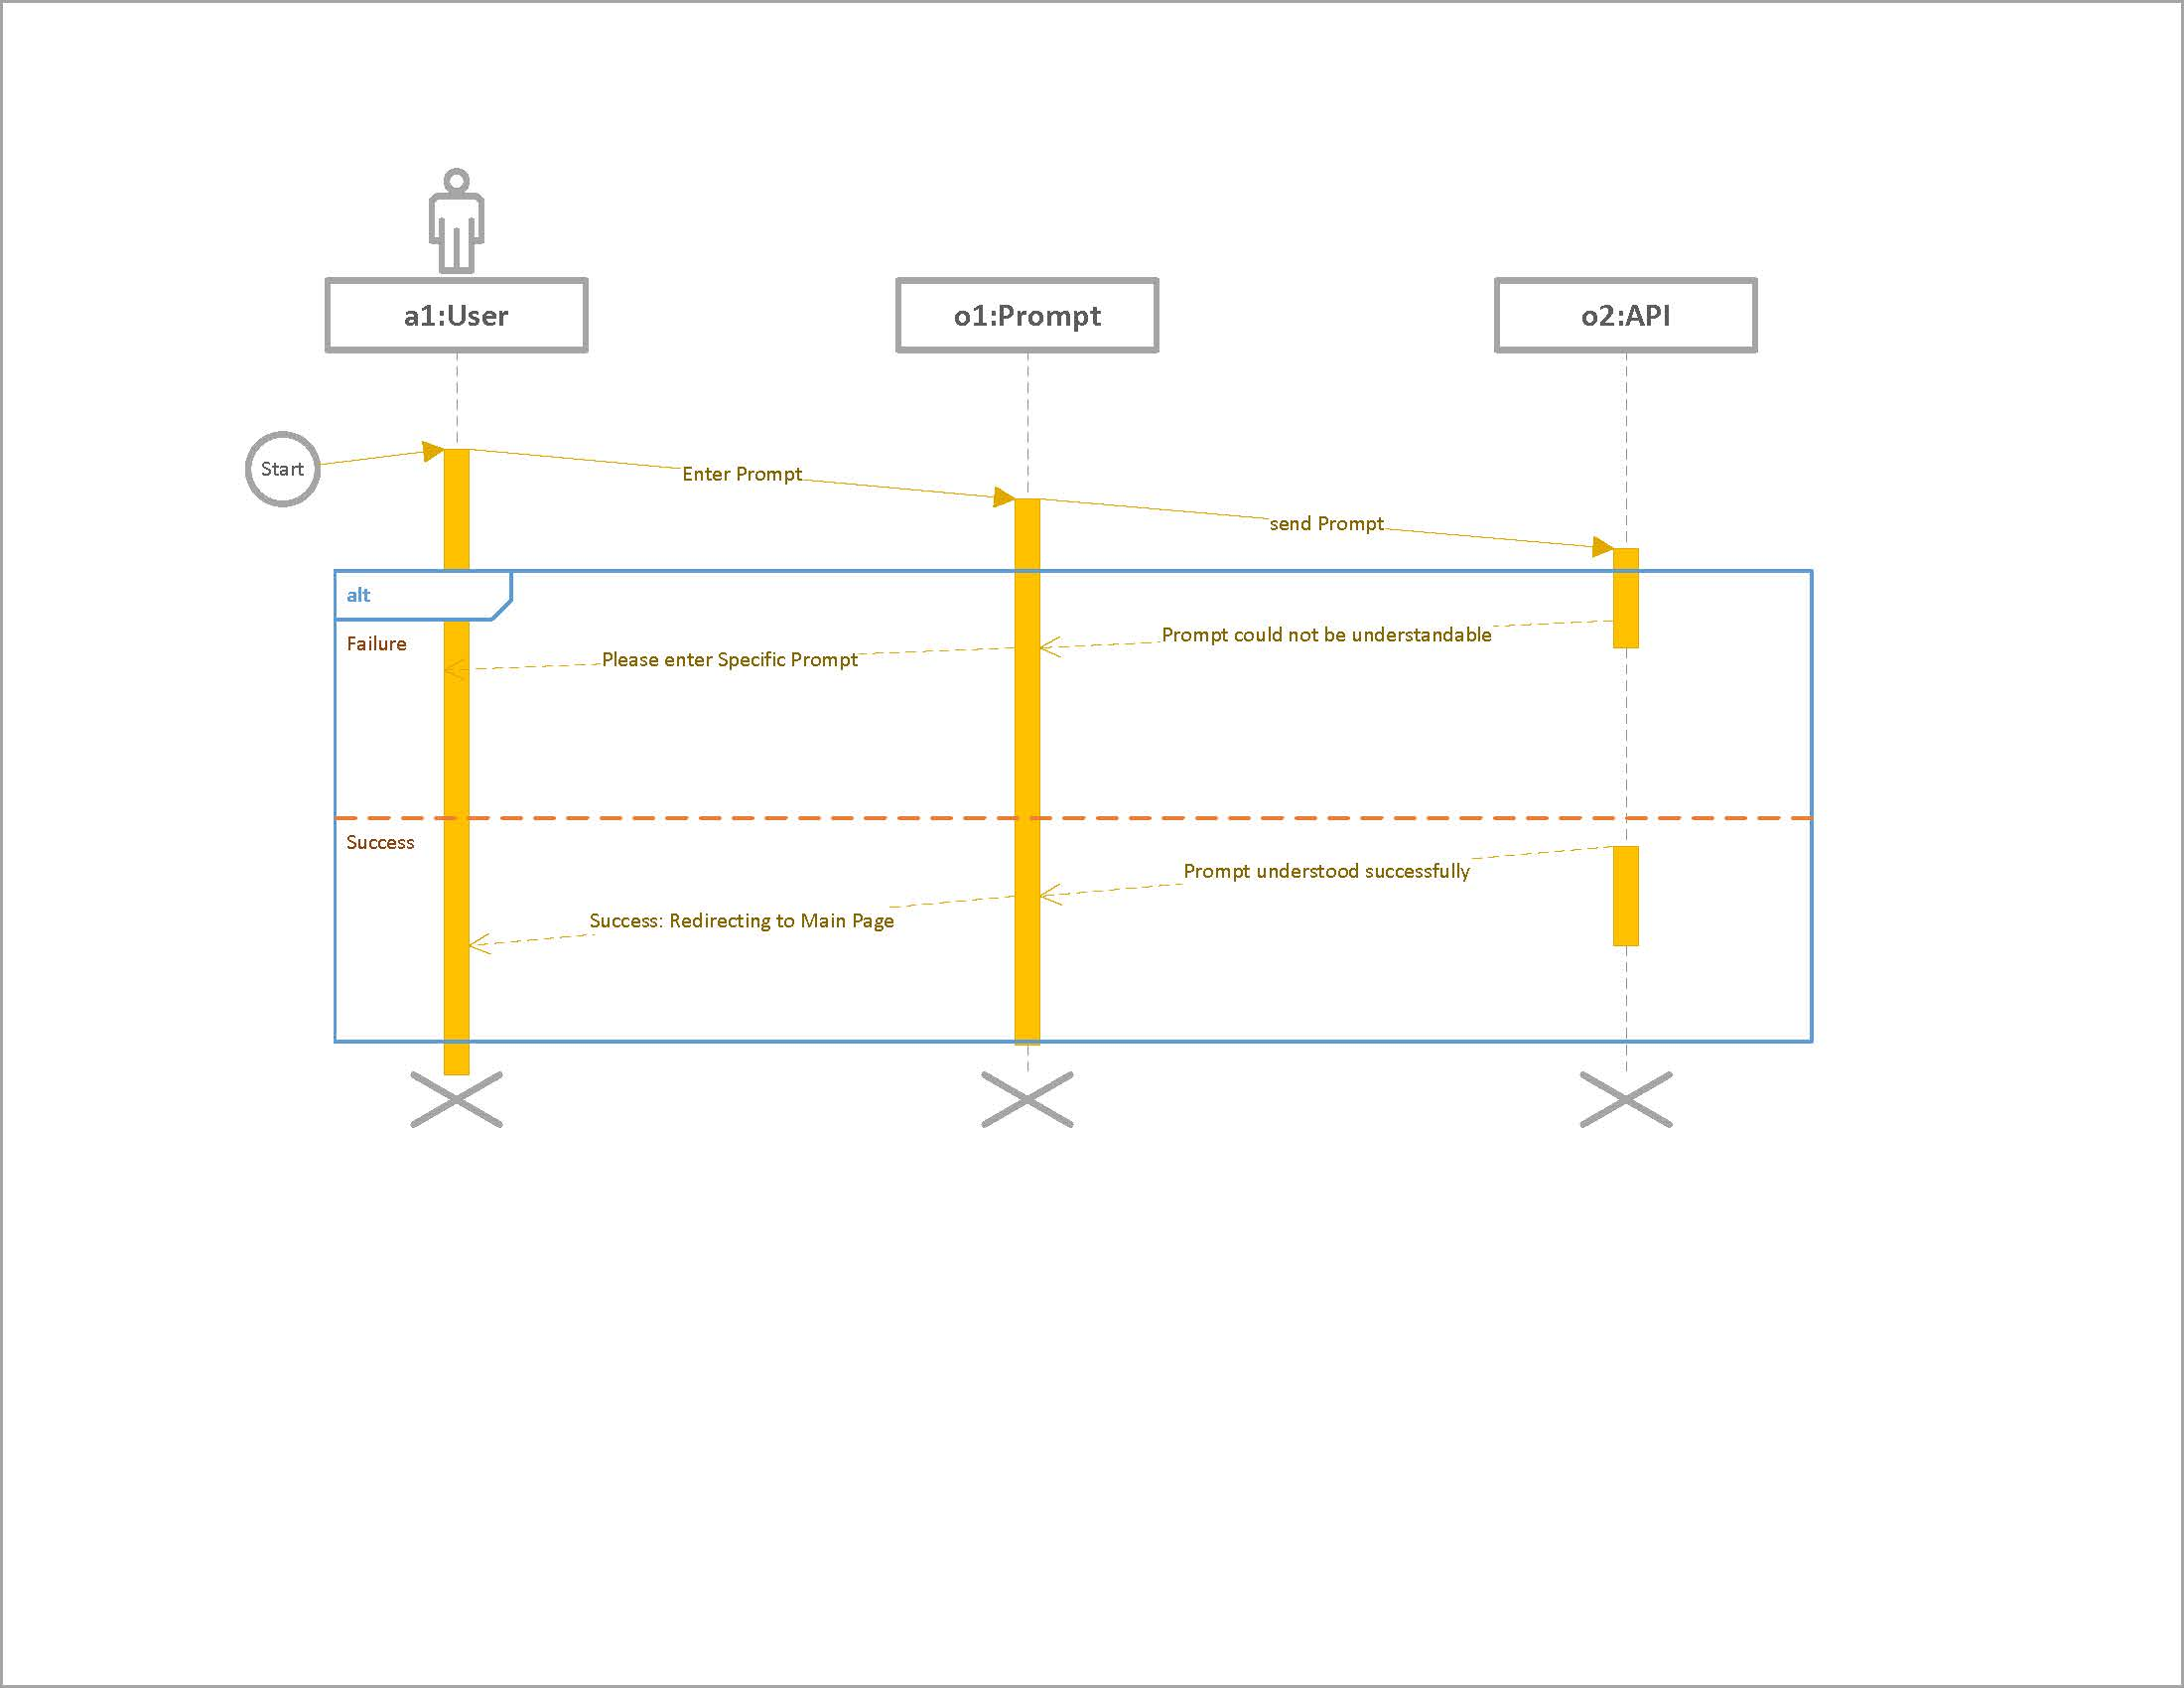
\includegraphics[width=0.8\textwidth]{Media/s1_Page_01.jpg} % Path to your image
    \caption{Sequence Diagram: Prompt (User)}
    
    \label{fig:drawing1}
\end{figure}
\begin{figure}[ht]
    \centering
    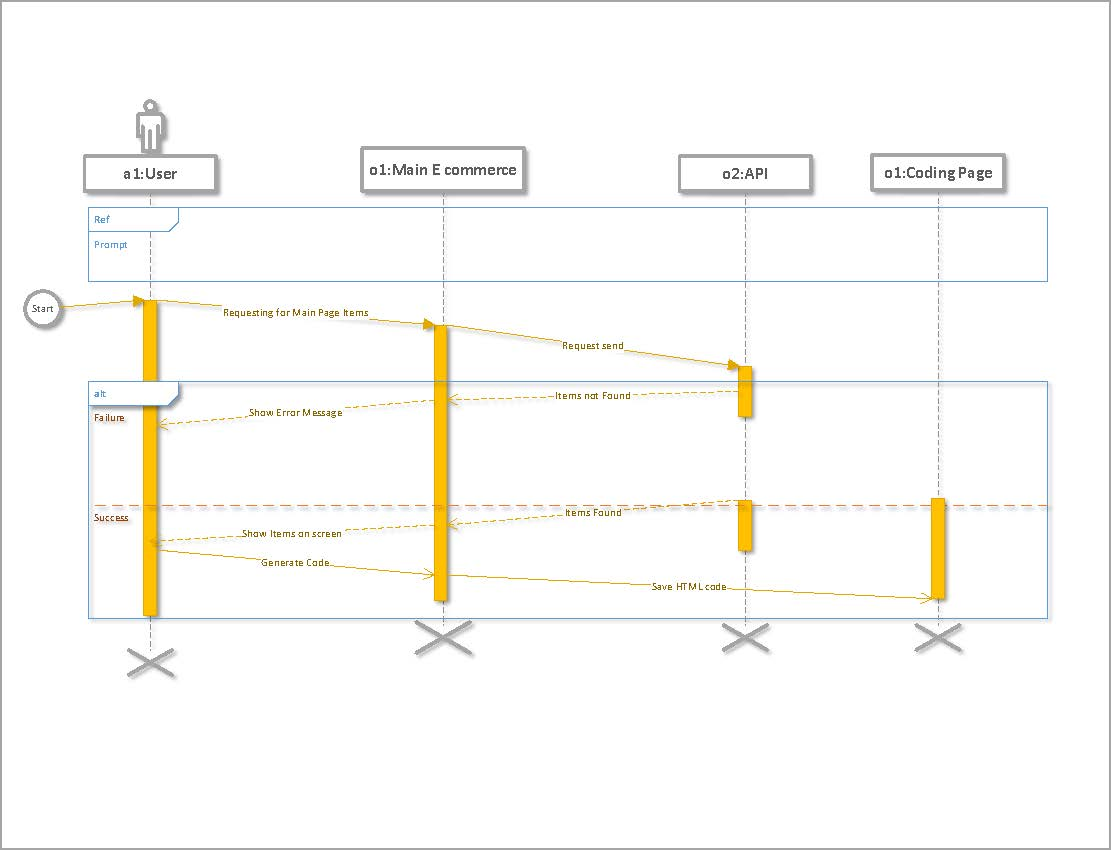
\includegraphics[width=0.8\textwidth]{Media/s1_Page_02.jpg} % Path to your image
    \caption{Sequence Diagram: Main of E-commerce a (User)}
    \label{fig:drawing1}
\end{figure}
\begin{figure}[ht]
    \centering
    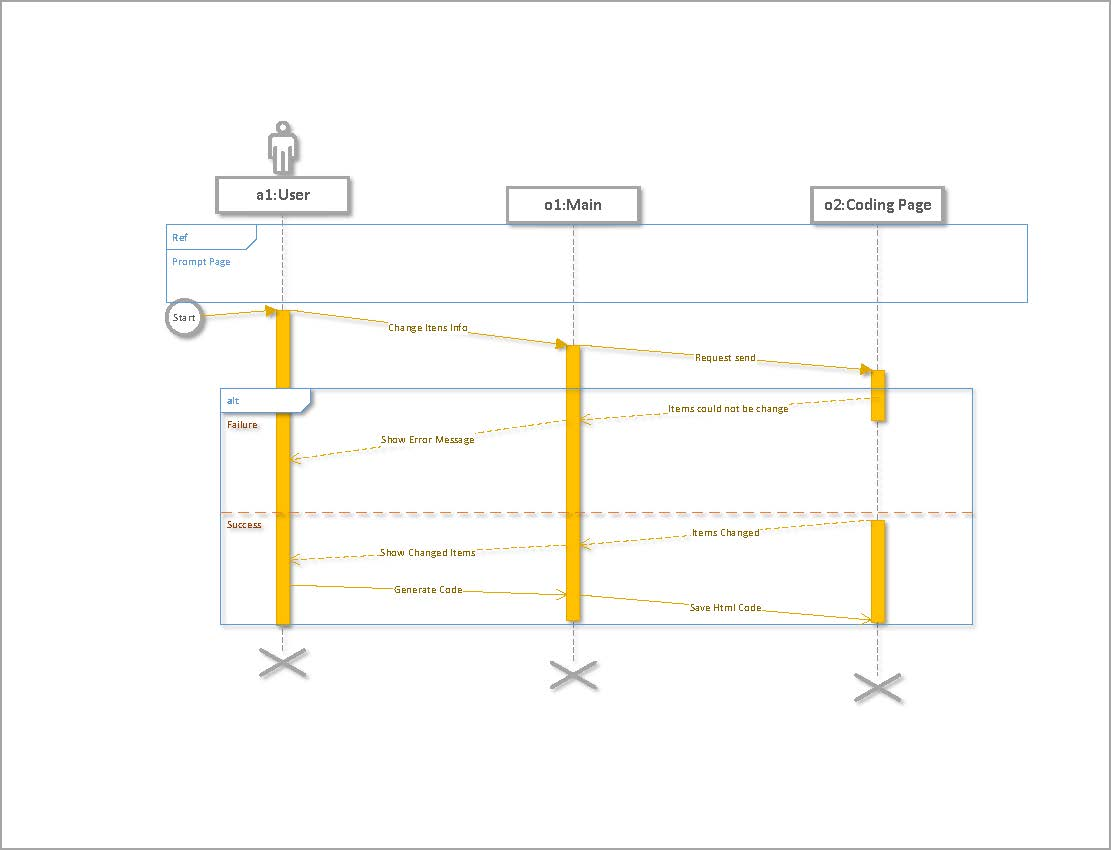
\includegraphics[width=0.8\textwidth]{Media/s1_Page_03.jpg} % Path to your image
    \caption{Sequence Diagram: Main of  E-commerce b (User)}
    \label{fig:drawing1}
\end{figure}

\begin{figure}[ht]
    \centering
    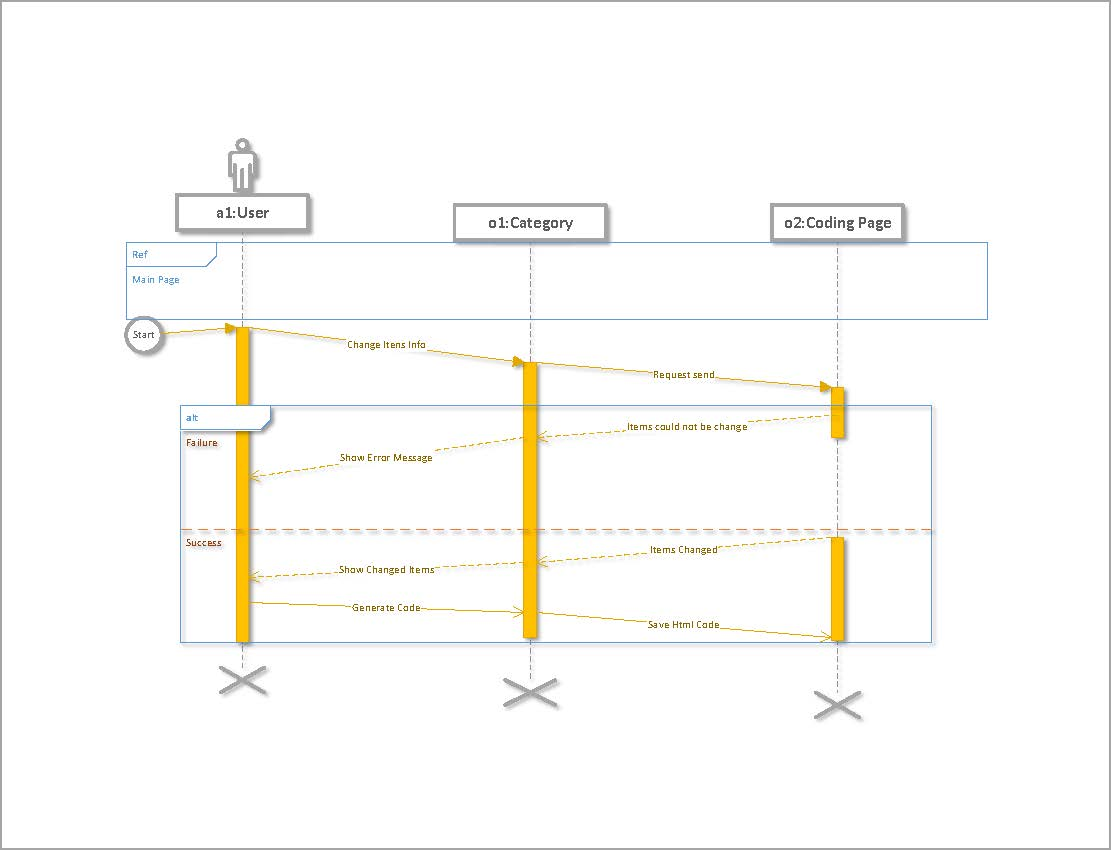
\includegraphics[width=0.8\textwidth]{Media/s1_Page_04.jpg} % Path to your image
    \caption{Sequence Diagram: Category of E-commerce a (User)}
    \label{fig:drawing1}
\end{figure}

\begin{figure}[ht]
    \centering
    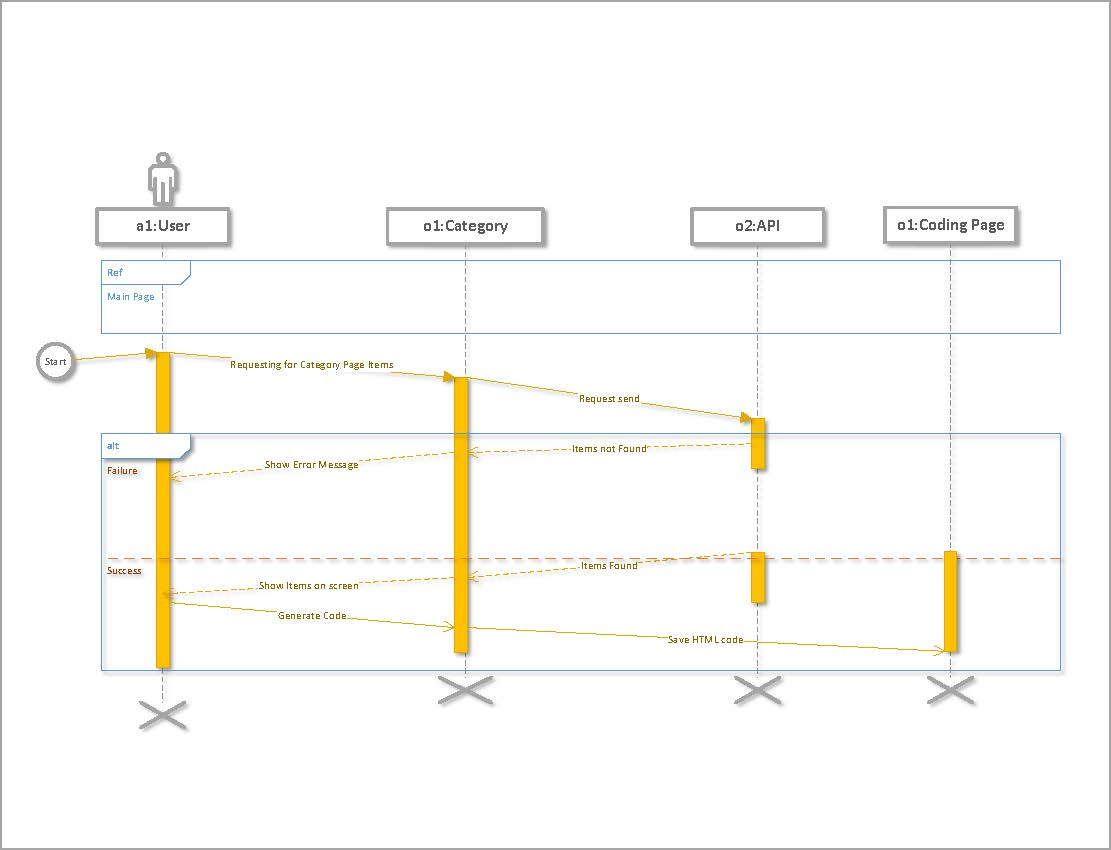
\includegraphics[width=0.8\textwidth]{Media/s1_Page_05.jpg} % Path to your image
    \caption{Sequence Diagram: Category of E-commerce b (User)}
    \label{fig:drawing1}
\end{figure}

\begin{figure}[ht]
    \centering
    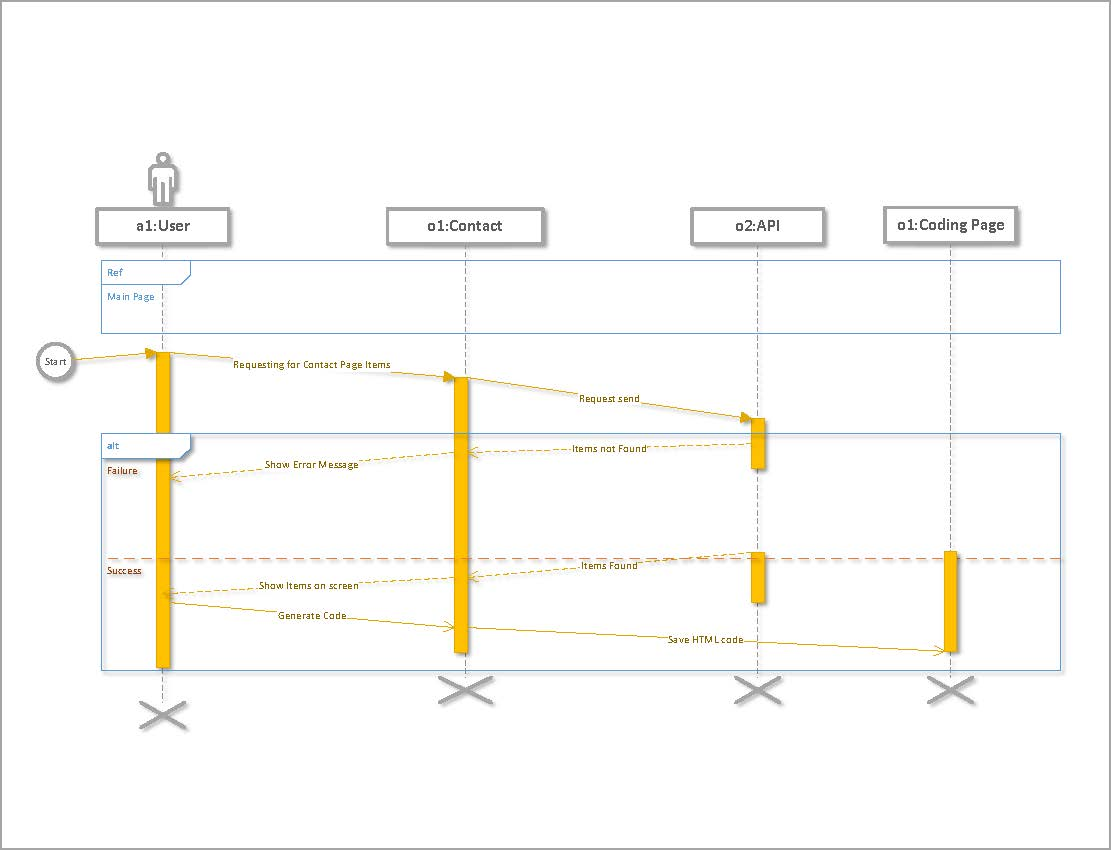
\includegraphics[width=0.8\textwidth]{Media/s1_Page_06.jpg} % Path to your image
    \caption{Sequence Diagram: Contact of E-commerce, Blogs and Porfolio a (User)}
    \label{fig:drawing1}
\end{figure}

\begin{figure}[ht]
    \centering
    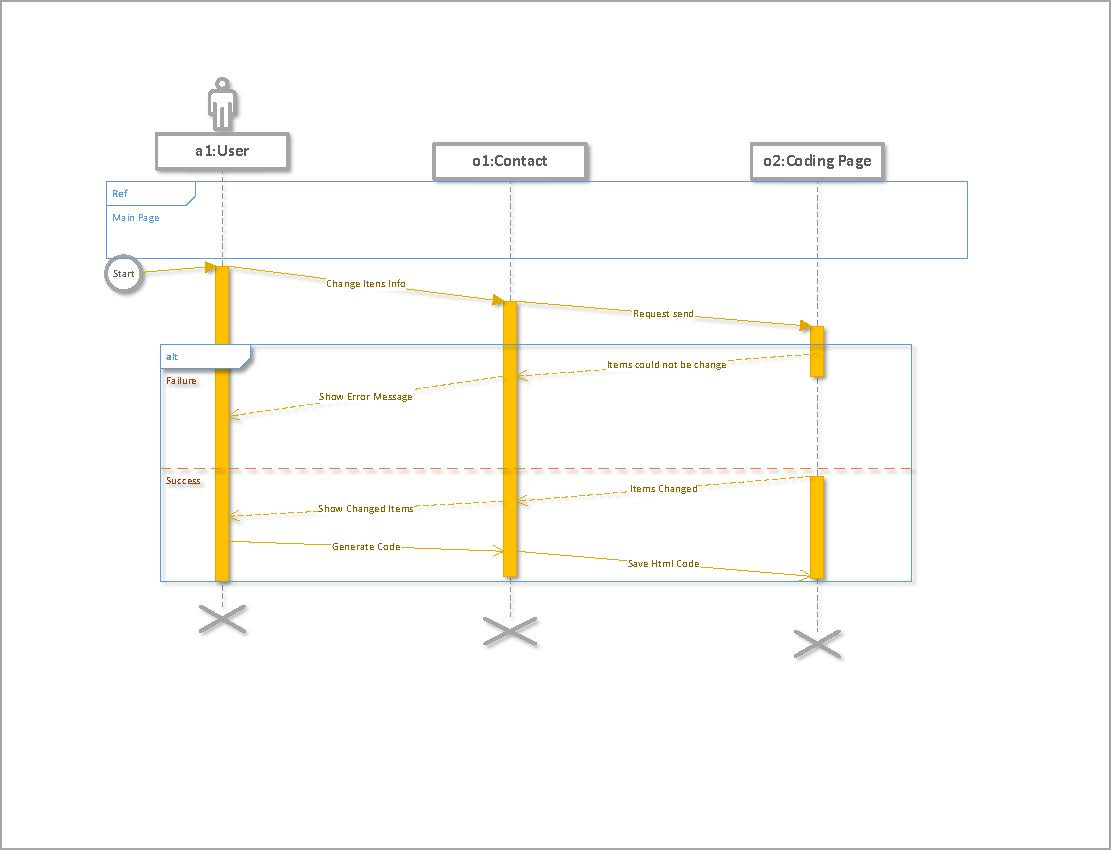
\includegraphics[width=0.8\textwidth]{Media/s1_Page_07.jpg} % Path to your image
    \caption{Sequence Diagram: Contact of E-commerce, Blogs and Porfolio b (User)}
    \label{fig:drawing1}
\end{figure}

\begin{figure}[ht]
    \centering
    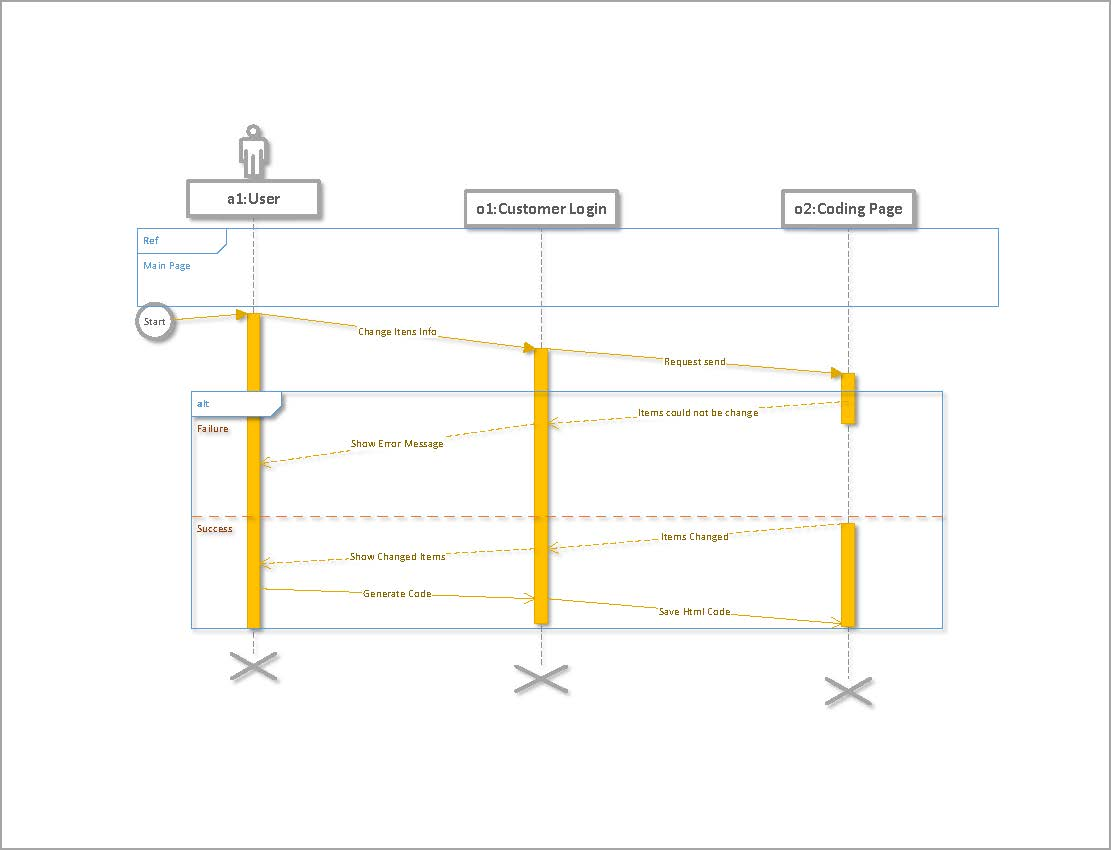
\includegraphics[width=0.8\textwidth]{Media/s1_Page_08.jpg} % Path to your image
    \caption{Sequence Diagram: Customer login of E-commerce a (User)}
    \label{fig:drawing1}
\end{figure}

\begin{figure}[ht]
    \centering
    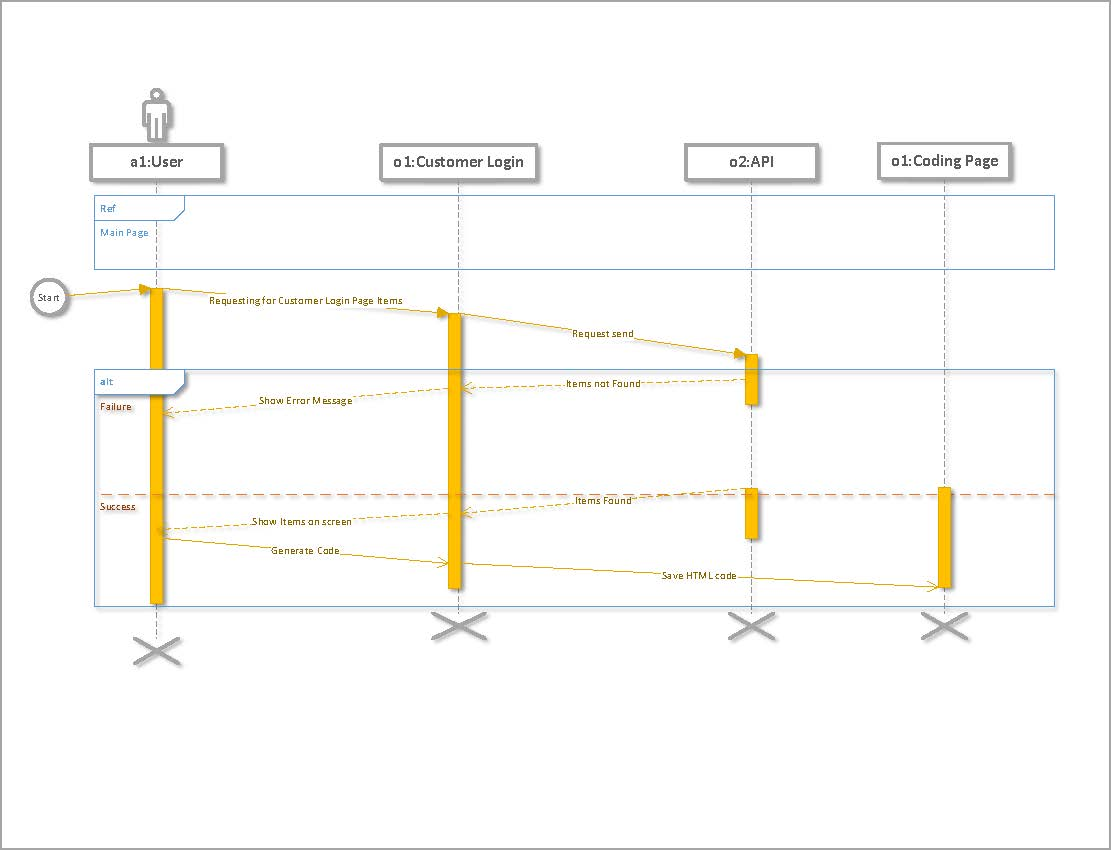
\includegraphics[width=0.8\textwidth]{Media/s1_Page_09.jpg} % Path to your image
    \caption{Sequence Diagram: Customer Login of E-commerce b (User)}
    \label{fig:drawing1}
\end{figure}

\begin{figure}[ht]
    \centering
    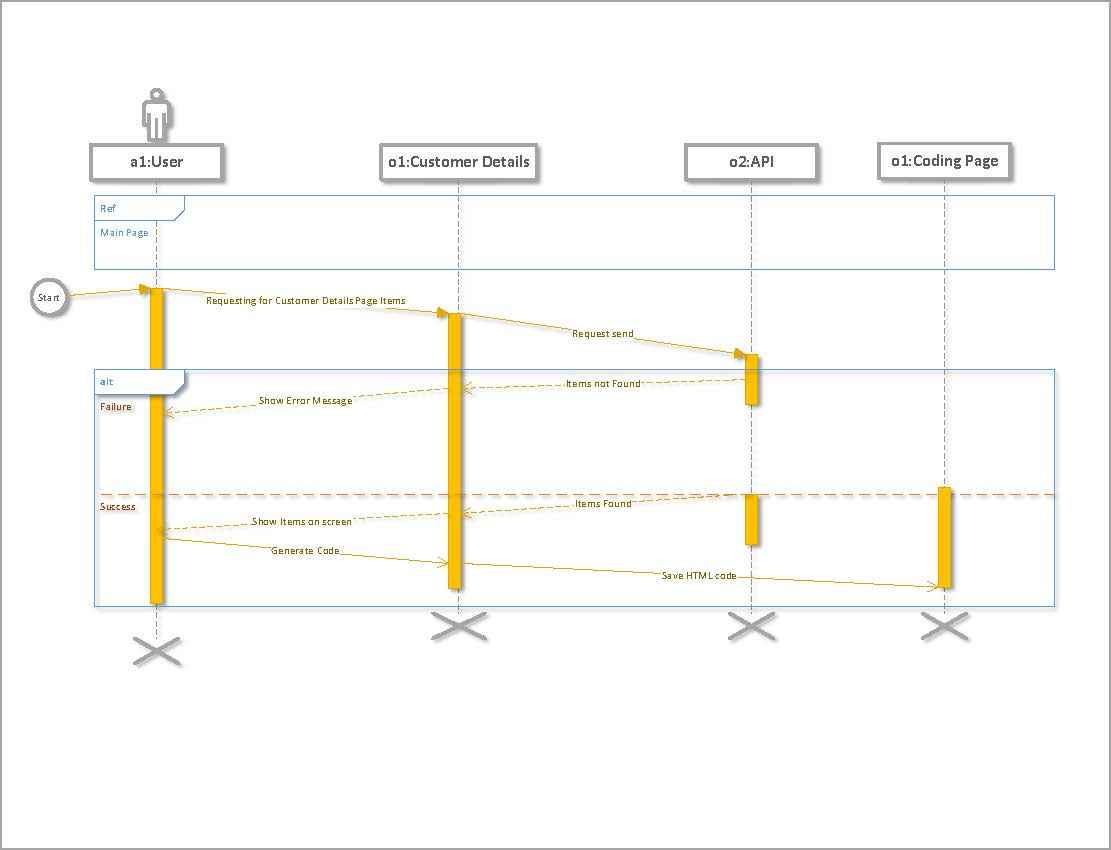
\includegraphics[width=0.8\textwidth]{Media/s1_Page_10.jpg} % Path to your image
    \caption{Sequence Diagram: Customer Details of E-commerce a (User)}
    \label{fig:drawing1}
\end{figure}

\begin{figure}[ht]
    \centering
    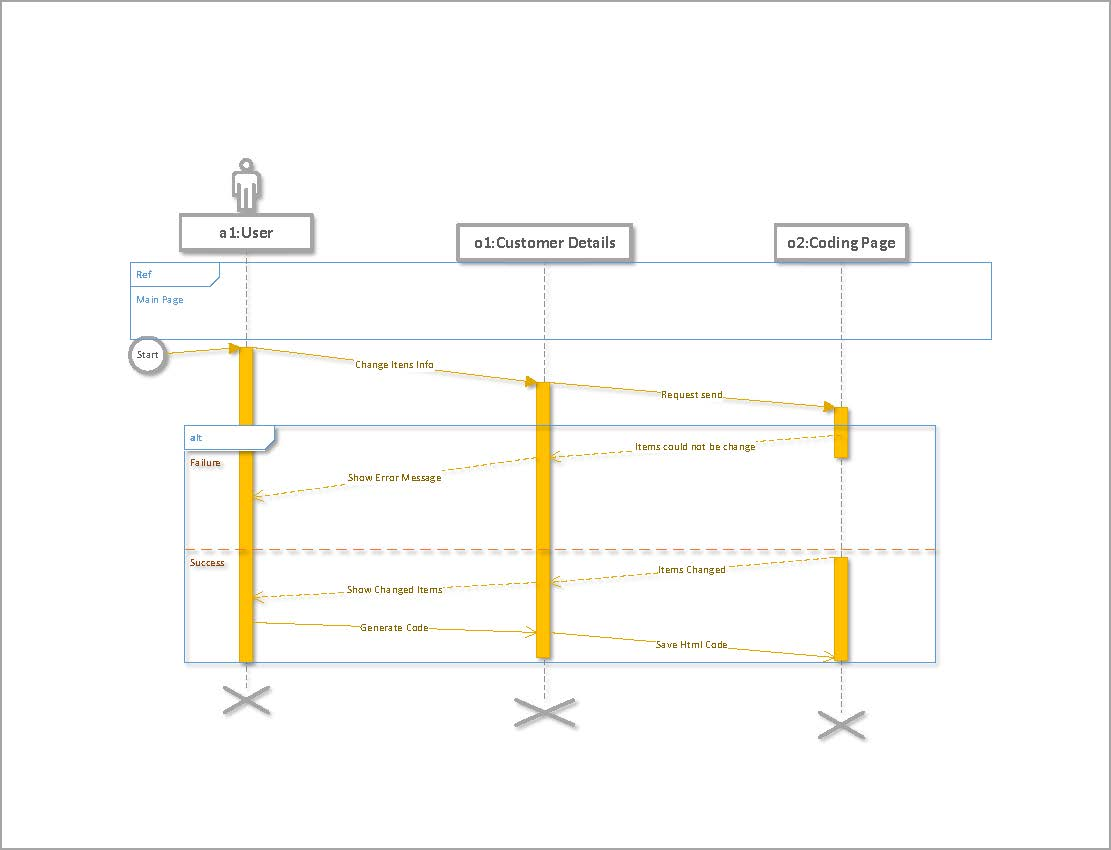
\includegraphics[width=0.8\textwidth]{Media/s1_Page_11.jpg} % Path to your image
    \caption{Sequence Diagram: Customer Details of E-commerce b (User)}
    \label{fig:drawing1}
\end{figure}

\begin{figure}[ht]
    \centering
    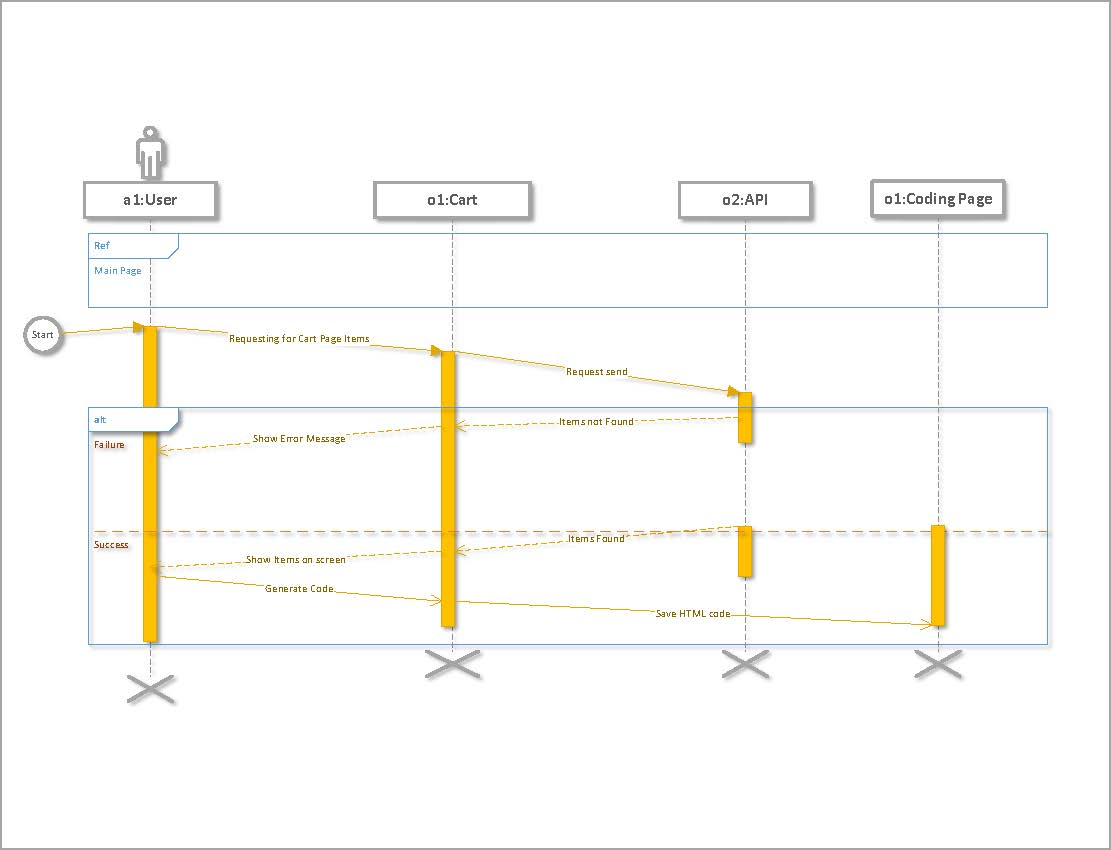
\includegraphics[width=0.8\textwidth]{Media/s1_Page_12.jpg} % Path to your image
    \caption{Sequence Diagram: Customer Details of E-commerce a (User)}
    \label{fig:drawing1}
\end{figure}

\begin{figure}[ht]
    \centering
    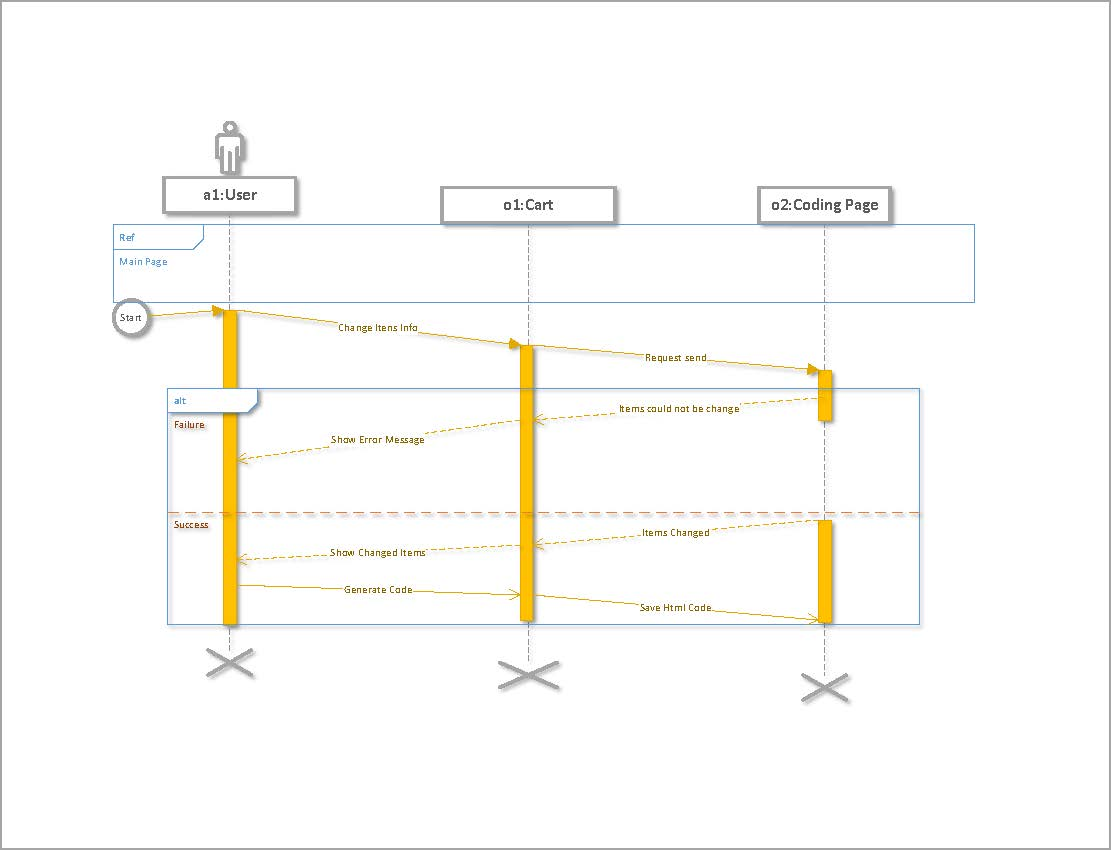
\includegraphics[width=0.8\textwidth]{Media/s1_Page_13.jpg} % Path to your image
    \caption{Sequence Diagram: Customer Details of E-commerce b (User)}
    \label{fig:drawing1}
\end{figure}

\begin{figure}[ht]
    \centering
    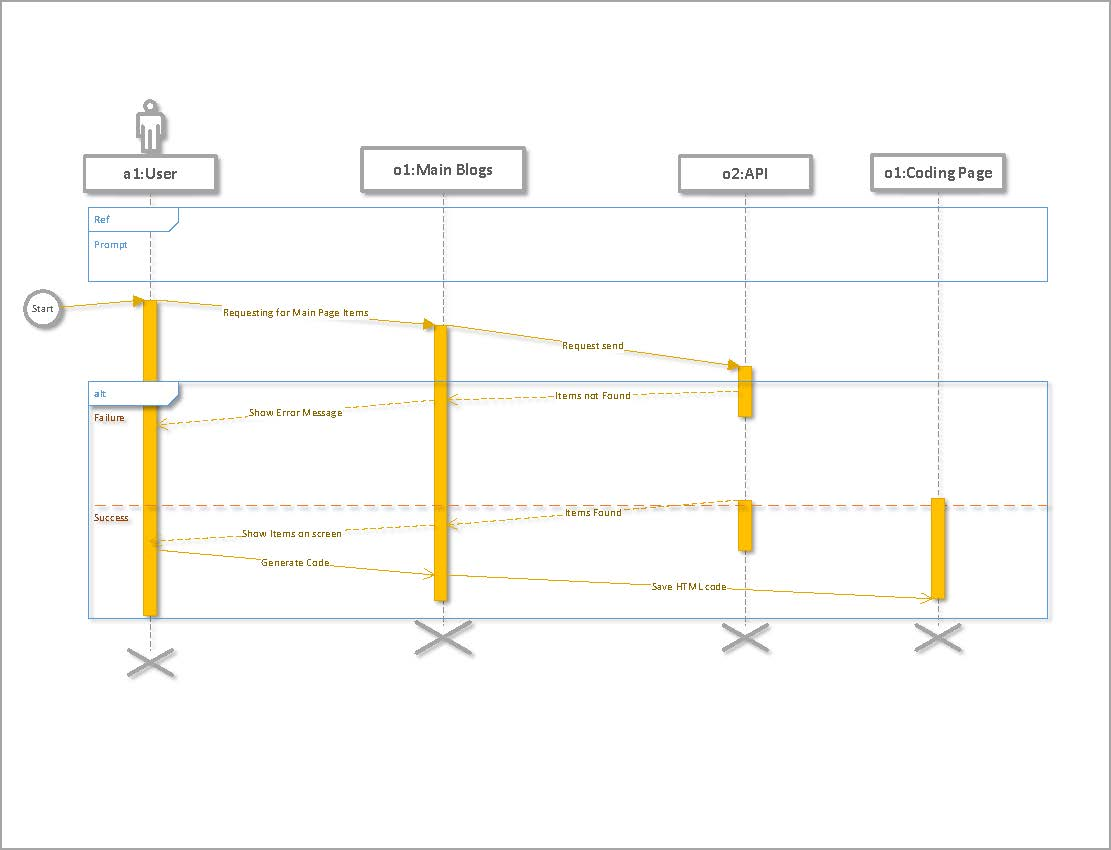
\includegraphics[width=0.8\textwidth]{Media/s1_Page_14.jpg} % Path to your image
    \caption{Sequence Diagram: Main of Blogs a (User)}
    \label{fig:drawing1}
\end{figure}

\begin{figure}[ht]
    \centering
    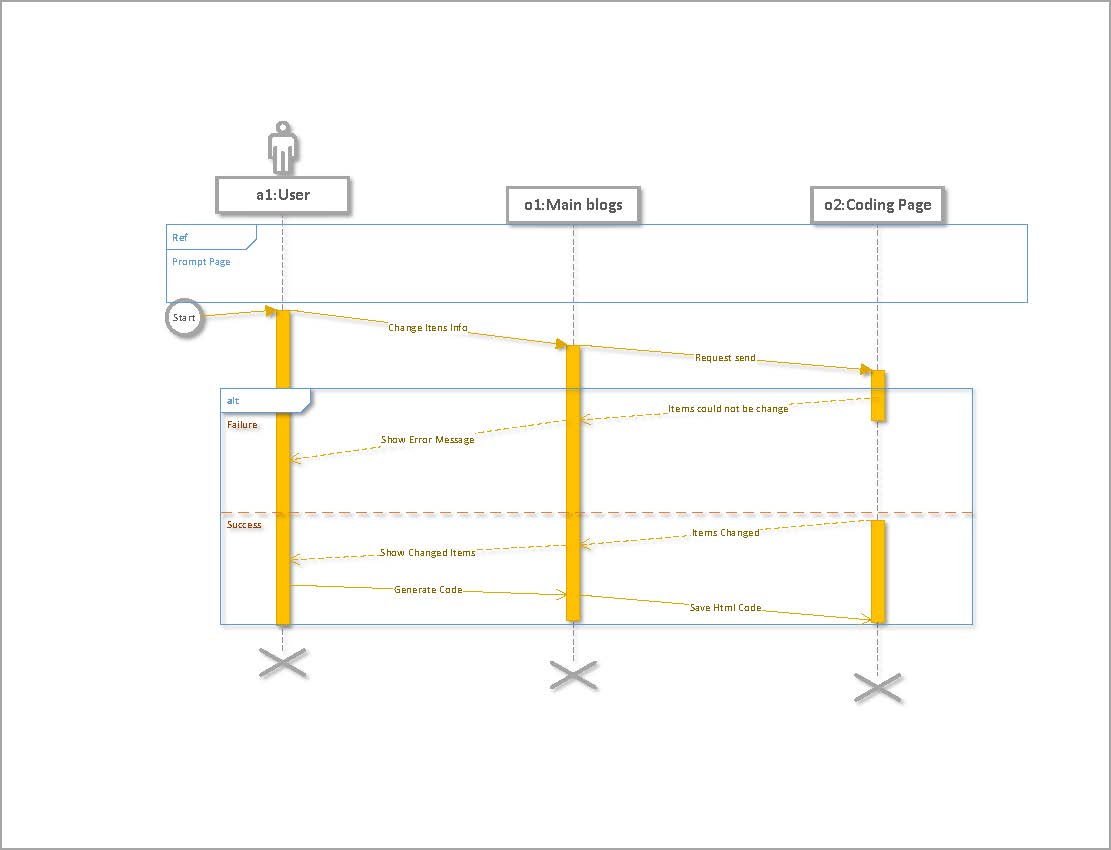
\includegraphics[width=0.8\textwidth]{Media/s1_Page_15.jpg} % Path to your image
    \caption{Sequence Diagram: Main of Blogs b (User)}
    \label{fig:drawing1}
\end{figure}

\begin{figure}[ht]
    \centering
    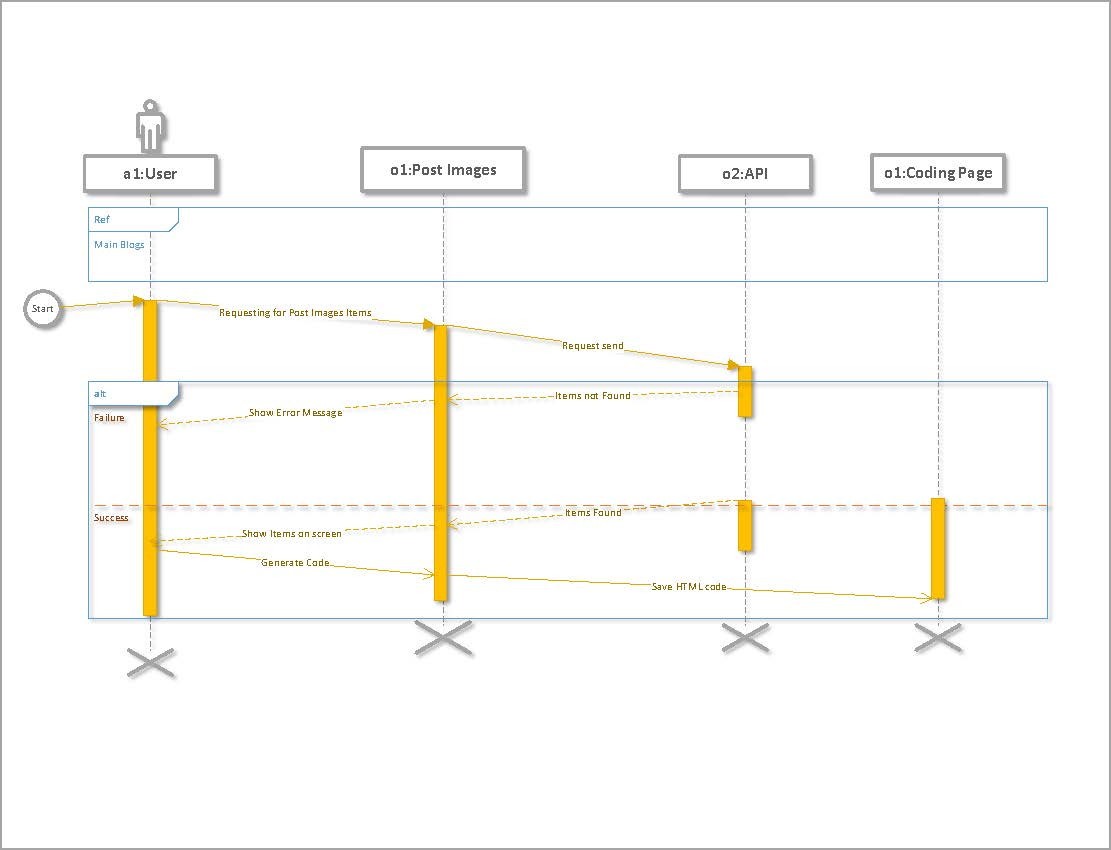
\includegraphics[width=0.8\textwidth]{Media/s1_Page_16.jpg} % Path to your image
    \caption{Sequence Diagram: Post Images of Blogs a (User)}
    \label{fig:drawing1}
\end{figure}

\begin{figure}[ht]
    \centering
    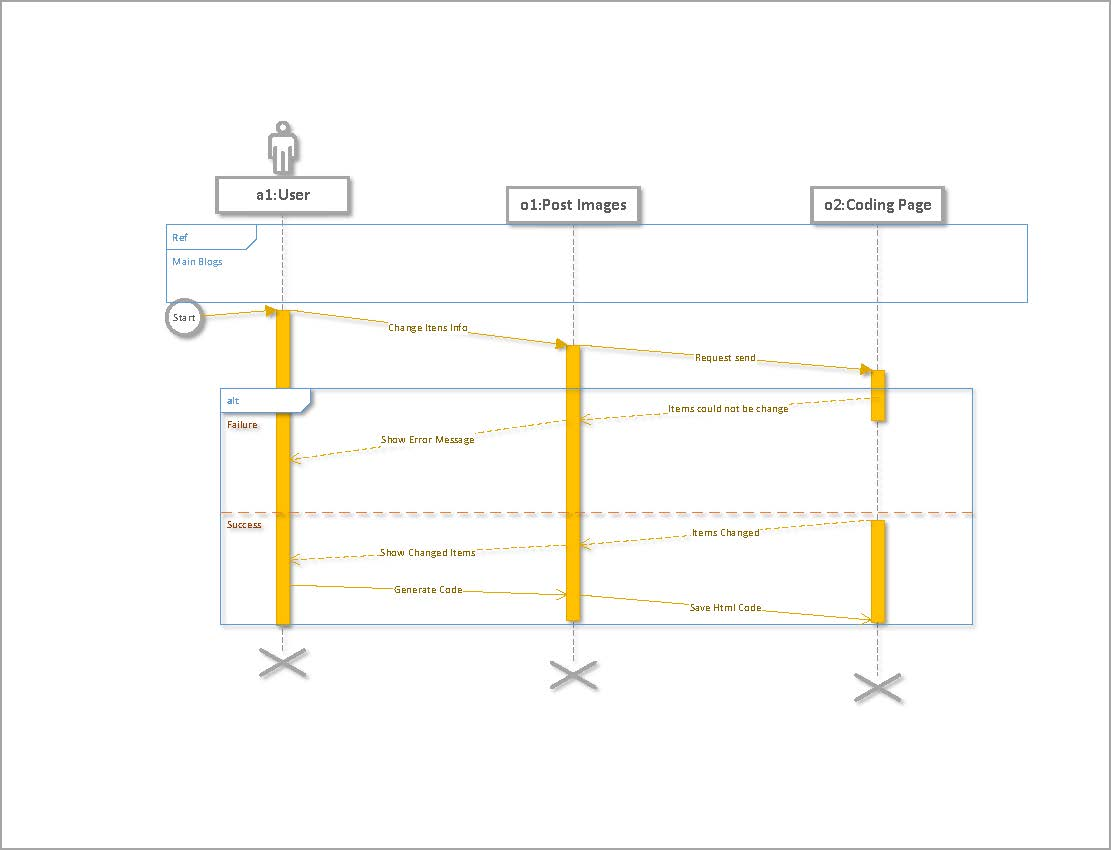
\includegraphics[width=0.8\textwidth]{Media/s1_Page_17.jpg} % Path to your image
    \caption{Sequence Diagram: Post Images of Blogs b (User)}
    \label{fig:drawing1}
\end{figure}

\begin{figure}[ht]
    \centering
    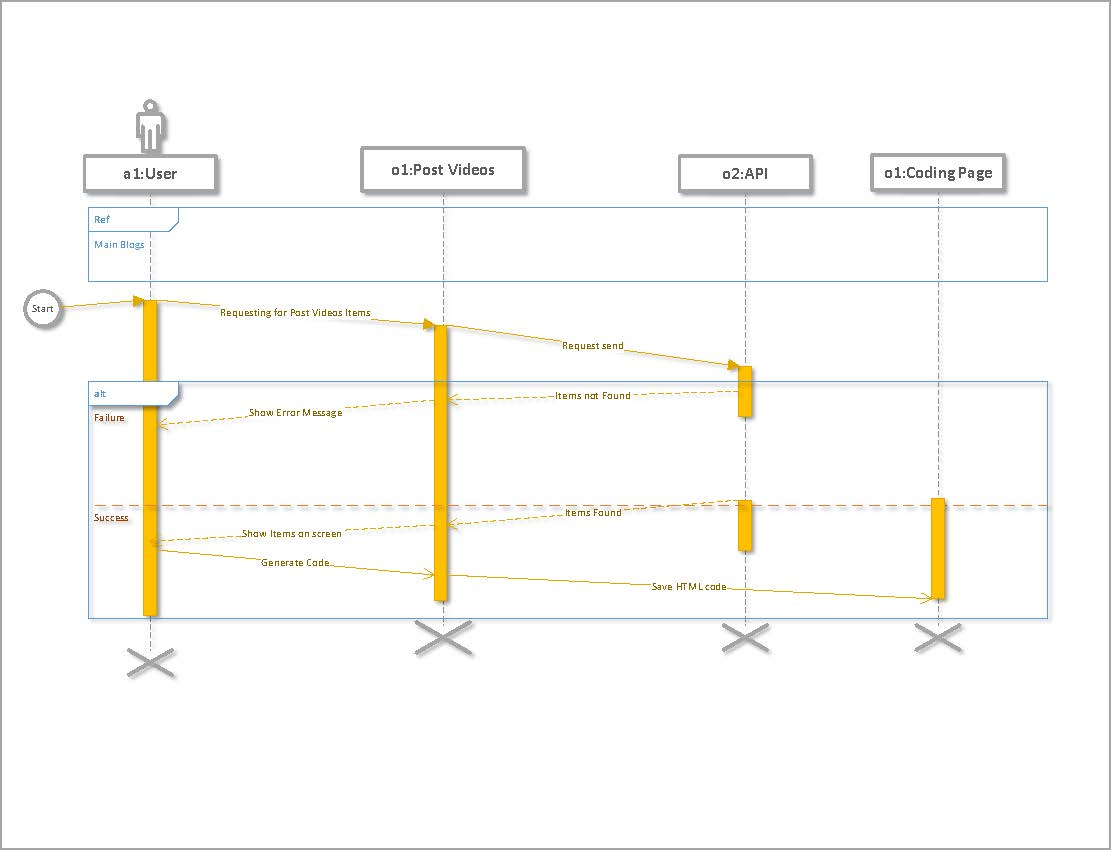
\includegraphics[width=0.8\textwidth]{Media/s1_Page_18.jpg} % Path to your image
    \caption{Sequence Diagram: Post Videos of Blogs a (User)}
    \label{fig:drawing1}
\end{figure}

\begin{figure}[ht]
    \centering
    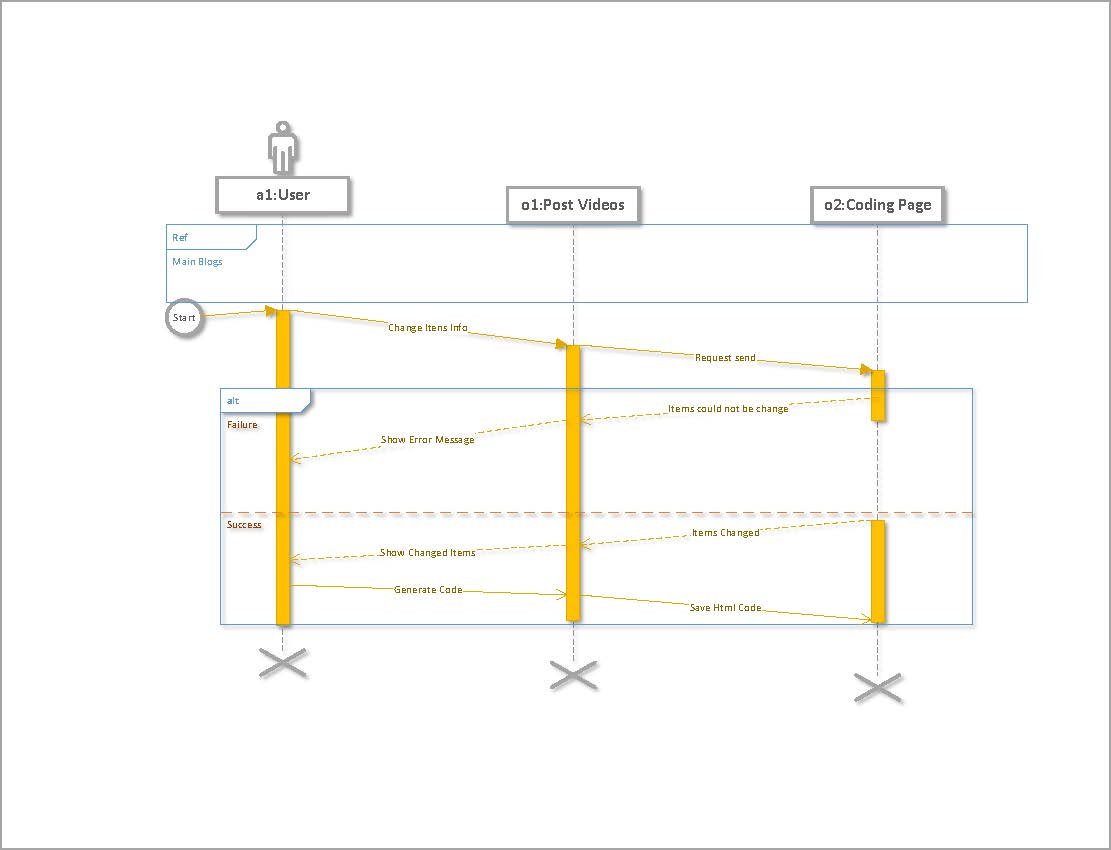
\includegraphics[width=0.8\textwidth]{Media/s1_Page_19.jpg} % Path to your image
    \caption{Sequence Diagram: Post Videos of Blogs b (User)}
    \label{fig:drawing1}
\end{figure}

% \begin{figure}[ht]
%     \centering
%     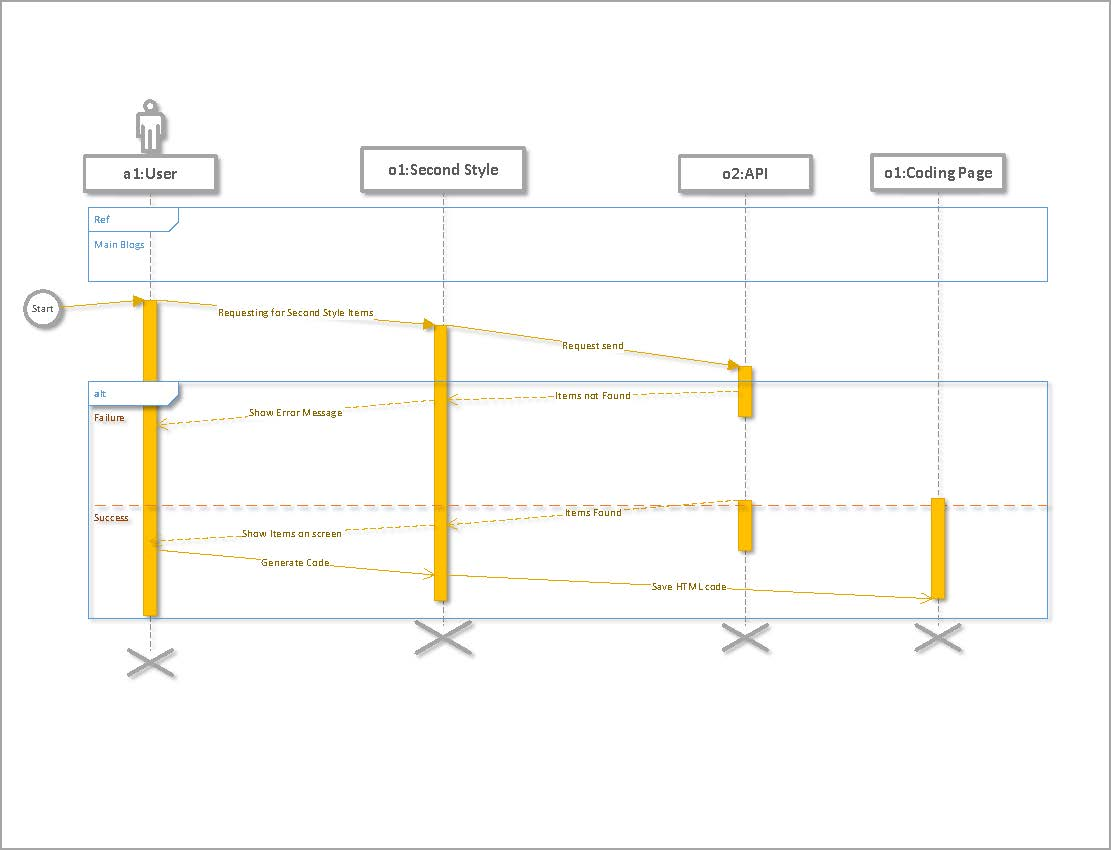
\includegraphics[width=0.8\textwidth]{Media/s1_Page_20.jpg} % Path to your image
%     \caption{Deployment Diagram}
%     \label{fig:drawing1}
% \end{figure}

% \begin{figure}[ht]
%     \centering
%     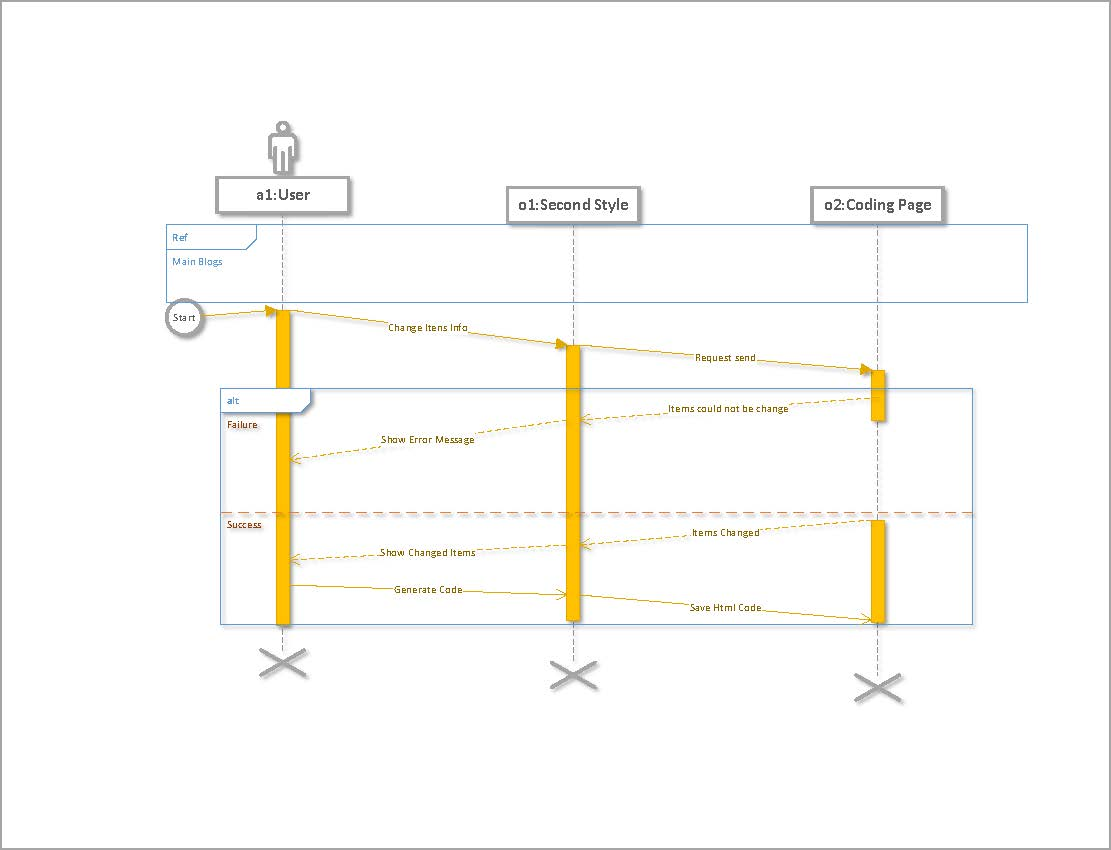
\includegraphics[width=0.8\textwidth]{Media/s1_Page_21.jpg} % Path to your image
%     \caption{Deployment Diagram}
%     \label{fig:drawing1}
% \end{figure}

\begin{figure}[ht]
    \centering
    \includegraphics[width=0.8\textwidth]{Media/s1_Page_22.jpg} % Path to your image
    \caption{Sequence Diagram: Main of Portfolio a (User)}
    \label{fig:drawing1}
\end{figure}

\begin{figure}[ht]
    \centering
    \includegraphics[width=0.8\textwidth]{Media/s1_Page_23.jpg} % Path to your image
    \caption{Sequence Diagram: Main of Portfolio b (User)}
    \label{fig:drawing1}
\end{figure}

\begin{figure}[ht]
    \centering
    \includegraphics[width=0.8\textwidth]{Media/s1_Page_24.jpg} % Path to your image
    \caption{Sequence Diagram: Projects of Portfolio a (User)}
    \label{fig:drawing1}
\end{figure}

\begin{figure}[ht]
    \centering
    \includegraphics[width=0.8\textwidth]{Media/s1_Page_25.jpg} % Path to your image
    \caption{Sequence Diagram: SignUp (User)}
    \label{fig:drawing1}
\end{figure}

\begin{figure}[ht]
    \centering
    \includegraphics[width=0.8\textwidth]{Media/s1_Page_26.jpg} % Path to your image
    \caption{Sequence Diagram: SignIn (User)}
    \label{fig:drawing1}
\end{figure}

\begin{figure}[ht]
    \centering
    \includegraphics[width=0.8\textwidth]{Media/s1_Page_27.jpg} % Path to your image
    \caption{Sequence Diagram: Contact Us (User)}
    \label{fig:drawing1}
\end{figure}



\begin{figure}[ht]
    \centering
    \includegraphics[width=0.8\textwidth]{Media/s1_Page_29.jpg} % Path to your image
    \caption{Sequence Diagram: SignUp (Admin)}
    \label{fig:drawing1}
\end{figure}

\begin{figure}[ht]
    \centering
    \includegraphics[width=0.8\textwidth]{Media/s1_Page_30.jpg} % Path to your image
    \caption{Sequence Diagram: SignIn (Admin)}
    \label{fig:drawing1}
\end{figure}

\begin{figure}[ht]
    \centering
    \includegraphics[width=0.8\textwidth]{Media/s1_Page_32.jpg} % Path to your image
    \caption{Sequence Diagram: Manage Template (Admin)}
    \label{fig:drawing1}
\end{figure}




\clearpage
    % Remaining
\subsection{Collaboration Diagram}

% \begin{figure}[ht]
%     \centering
%     \includegraphics[width=0.8\textwidth]{Media/c1_Page_01.jpg} % Path to your image
%     \caption{Deployment Diagram}
%     \label{fig:drawing1}
% \end{figure}

\begin{figure}[ht]
    \centering
    \includegraphics[width=1\textwidth, trim=4cm 1.5cm 4cm 2cm, clip]{Media/c1_Page_ 2.pdf} % Path to your image
    \caption{Collaboration Diagram: Prompt (User)}
    \label{fig:drawing1}
\end{figure}

\begin{figure}[ht]
    \centering
    \includegraphics[width=0.8\textwidth, trim=4cm 3cm 4cm 3cm, clip]{Media/c1_Page_ 3.pdf} % Path to your image
    \caption{Collaboration Diagram: Main of E commerce,Blogs and Portfolio a (User)}
    \label{fig:drawing1}
\end{figure}

\begin{figure}[ht]
    \centering
    \includegraphics[width=0.8\textwidth, trim=4cm 3cm 4cm 2cm, clip]{Media/c1_Page_ 4.pdf} % Path to your image
    \caption{Collaboration Diagram: Main of E commerce,Blogs and Portfolio b (User)}
    \label{fig:drawing1}
\end{figure}

\begin{figure}[ht]
    \centering
    \includegraphics[width=0.8\textwidth, trim=4cm 3cm 4cm 2cm, clip]{Media/c1_Page_ 5.pdf} % Path to your image
    \caption{Collaboration Diagram: Category of E commerce,Blogs and Portfolio a (User)}
    \label{fig:drawing1}
\end{figure}

\begin{figure}[ht]
    \centering
    \includegraphics[width=0.8\textwidth, trim=4cm 3cm 4cm 2cm, clip]{Media/c1_Page_ 6.pdf} % Path to your image
    \caption{Collaboration Diagram: Category of E commerce,Blogs and Portfolio b (User)}
    \label{fig:drawing1}
\end{figure}

\begin{figure}[ht]
    \centering
    \includegraphics[width=0.8\textwidth, trim=4cm 3cm 4cm 2cm, clip]{Media/c1_Page_ 7.pdf} % Path to your image
    \caption{Collaboration Diagram: Contact of E commerce,Blogs and Portfolio a (User)}
    \caption{}
    \label{fig:drawing1}
\end{figure}

\begin{figure}[ht]
    \centering
    \includegraphics[width=0.8\textwidth, trim=4cm 3cm 4cm 2cm, clip]{Media/c1_Page_ 8.pdf} % Path to your image
    \caption{Collaboration Diagram: Contact of E commerce,Blogs and Portfolio b (User)}
    \label{fig:drawing1}
\end{figure}

\begin{figure}[ht]
    \centering
    \includegraphics[width=0.8\textwidth, trim=4cm 3cm 4cm 2cm, clip]{Media/c1_Page_ 9.pdf} % Path to your image
    \caption{Collaboration Diagram: Customer login of E commerce a (User)}
    \label{fig:drawing1}
\end{figure}

\begin{figure}[ht]
    \centering
    \includegraphics[width=0.8\textwidth, trim=4cm 3cm 4cm 2cm, clip]{Media/c1_Page_ 10.pdf} % Path to your image
    \caption{Collaboration Diagram: Customer login of E commerce a (User)}
    \label{fig:drawing1}
\end{figure}

% \begin{figure}[ht]
%     \centering
%     \includegraphics[width=0.8\textwidth]{Media/c1_Page_11.jpg} % Path to your image
%     \caption{Collaboration Diagram: Customer login of E commerce b (User)}
%     \label{fig:drawing1}
% \end{figure}

% % \begin{figure}[ht]
%     \centering
%     \includegraphics[width=0.8\textwidth]{Media/c1_Page_12.jpg} % Path to your image
%     \caption{Deployment Diagram}
%     \label{fig:drawing1}
% \end{figure}

% \begin{figure}[ht]
%     \centering
%     \includegraphics[width=0.8\textwidth]{Media/c1_Page_13.jpg} % Path to your image
%     \caption{Deployment Diagram}
%     \label{fig:drawing1}
% \end{figure}

% \begin{figure}[ht]
%     \centering
%     \includegraphics[width=0.8\textwidth]{Media/c1_Page_14.jpg} % Path to your image
%     \caption{Collaboration Diagram: Cart of E commerce a (User)}
%     \label{fig:drawing1}
% \end{figure}

% \begin{figure}[ht]
%     \centering
%     \includegraphics[width=0.8\textwidth]{Media/c1_Page_15.jpg} % Path to your image
%     \caption{Collaboration Diagram: Cart of E commerce b (User)}
%     \label{fig:drawing1}
% \end{figure}

% \begin{figure}[ht]
%     \centering
%     \includegraphics[width=0.8\textwidth]{Media/c1_Page_16.jpg} % Path to your image
%     \caption{Deployment Diagram}
%     \label{fig:drawing1}
% \end{figure}

% \begin{figure}[ht]
%     \centering
%     \includegraphics[width=0.8\textwidth]{Media/c1_Page_17.jpg} % Path to your image
%     \caption{Deployment Diagram}
%     \label{fig:drawing1}
% \end{figure}

\begin{figure}[ht]
    \centering
    \includegraphics[width=0.8\textwidth, trim=4cm 3cm 4cm 2cm, clip]{Media/c1_Page_ 18.pdf} % Path to your image
    \caption{Collaboration Diagram: Post Image of E Blogs a (User)}
    \label{fig:drawing1}
\end{figure}

\begin{figure}[ht]
    \centering
    \includegraphics[width=0.8\textwidth, trim=4cm 3cm 4cm 2cm, clip]{Media/c1_Page_ 19.pdf} % Path to your image
    \caption{Collaboration Diagram: Post Image of Blogs b (User)}
    \label{fig:drawing1}
\end{figure}

\begin{figure}[ht]
    \centering
    \includegraphics[width=0.8\textwidth, trim=4cm 3cm 4cm 2cm, clip]{Media/c1_Page_ 20.pdf} % Path to your image
    \caption{Collaboration Diagram: Post Videos of Blogs a (User)}
    \label{fig:drawing1}
\end{figure}

\begin{figure}[ht]
    \centering
    \includegraphics[width=0.8\textwidth, trim=4cm 3cm 4cm 2cm, clip]{Media/c1_Page_ 21.pdf} % Path to your image
    \caption{Collaboration Diagram: Post Videos of Blogs b (User)}
    \label{fig:drawing1}
\end{figure}

% \begin{figure}[ht]
%     \centering
%     \includegraphics[width=0.8\textwidth]{Media/c1_Page_22.jpg} % Path to your image
%     \caption{Collaboration Diagram: Post Videos of Blogs a (User)}
%     \label{fig:drawing1}
% \end{figure}

% \begin{figure}[ht]
%     \centering
%     \includegraphics[width=0.8\textwidth]{Media/c1_Page_23.jpg} % Path to your image
%     \caption{Deployment Diagram}
%     \label{fig:drawing1}
% \end{figure}

% \begin{figure}[ht]
%     \centering
%     \includegraphics[width=0.8\textwidth]{Media/c1_Page_24.jpg} % Path to your image
%     \caption{Deployment Diagram}
%     \label{fig:drawing1}
% \end{figure}

% \begin{figure}[ht]
%     \centering
%     \includegraphics[width=0.8\textwidth]{Media/c1_Page_25.jpg} % Path to your image
%     \caption{Deployment Diagram}
%     \label{fig:drawing1}
% \end{figure}

\begin{figure}[ht]
    \centering
    \includegraphics[width=0.8\textwidth, trim=4cm 3cm 4cm 2cm, clip]{Media/c1_Page_ 26.pdf} % Path to your image
    \caption{Deployment Diagram}
    \label{fig:drawing1}
\end{figure}

\begin{figure}[ht]
    \centering
    \includegraphics[width=0.8\textwidth, trim=4cm 3cm 4cm 2cm, clip]{Media/c1_Page_ 27.pdf} % Path to your image
    \caption{Collaboration Diagram: Projects of Portfolio a (User)}
    \label{fig:drawing1}
\end{figure}

\begin{figure}[ht]
    \centering
    \includegraphics[width=0.8\textwidth, trim=4cm 3cm 4cm 2cm, clip]{Media/c1_Page_ 28.pdf} % Path to your image
    \caption{Collaboration Diagram: Projects of Portfolio b (User)}
    \label{fig:drawing1}
\end{figure}

\begin{figure}[ht]
    \centering
    \includegraphics[width=0.8\textwidth,, trim=4cm 3cm 4cm 2cm, clip]{Media/c1_Page_ 29.pdf} % Path to your image
    \caption{Collaboration Diagram: Sign Up (User)}
    \label{fig:drawing1}
\end{figure}

% \begin{figure}[ht]
%     \centering
%     \includegraphics[width=0.8\textwidth]{Media/c1_Page_30.jpg} % Path to your image
%     \caption{Collaboration Diagram: Sign In (User /Admin)}
%     \label{fig:drawing1}
% \end{figure}

\begin{figure}[ht]
    \centering
    \includegraphics[width=0.8\textwidth, trim=4cm 3cm 4cm 2cm, clip]{Media/c1_Page_ 31.pdf} % Path to your image
    \caption{Collaboration Diagram: Sign In (User )}
    \label{fig:drawing1}
\end{figure}

\begin{figure}[ht]
    \centering
    \includegraphics[width=0.8\textwidth, trim=4cm 3cm 4cm 2cm, clip]{Media/c1_Page_ 32.pdf} % Path to your image
    \caption{Collaboration Diagram: Contact Us (User )}
    \label{fig:drawing1}
\end{figure}

\begin{figure}[ht]
    \centering
    \includegraphics[width=0.8\textwidth, trim=4cm 3cm 4cm 2cm, clip]{Media/c1_Page_ 33.pdf} % Path to your image
    \caption{Collaboration Diagram: Sign Up (Admin)}
    \label{fig:drawing1}
\end{figure}

\begin{figure}[ht]
    \centering
    \includegraphics[width=0.8\textwidth, trim=4cm 3cm 4cm 2cm, clip]{Media/c1_Page_ 34.pdf} % Path to your image
    \caption{Collaboration Diagram: Sign In (Admin)}
    \label{fig:drawing1}
\end{figure}

% \begin{figure}[ht]
%     \centering
%     \includegraphics[width=0.8\textwidth]{Media/c1_Page_35.jpg} % Path to your image
%     \caption{Deployment Diagram}
%     \label{fig:drawing1}
% \end{figure}

\begin{figure}[ht]
    \centering
    \includegraphics[width=1\textwidth, trim=4cm 3cm 4cm 2cm, clip]{Media/c1_Page_ 36.pdf} % Path to your image
    \caption{Collaboration Diagram: Manage Templates (Admin)}
    \label{fig:drawing1}
\end{figure}


\clearpage

\section{System Structure Design}
\subsection{Class Diagram}

\begin{figure}[ht]
    \centering
    \includegraphics[width=1\textwidth]{Media/c.pdf} % Path to your image
    \caption{Class Diagram}
    \label{fig:drawing1}
\end{figure}
\clearpage
\subsection{Component Diagram}    % Remaining

\begin{figure}[ht]
    \centering
    \includegraphics[width=1\textwidth]{Media/com.jpg} % Path to your image
    \caption{Component Diagram}
    \label{fig:drawing1}
\end{figure}
\clearpage   % Remaining
\subsection{Deployment Diagram}

\begin{figure}[ht]
    \centering
    \includegraphics[width=1\textwidth, trim=0.1cm 0.1cm 0.1cm 0.1cm, clip]{Media/d.pdf} % Path to your image
    \caption{Deployment Diagram}
    \label{fig:drawing1}
\end{figure}
\clearpage







\clearpage
\section{Database Design}

\subsection{ER Diagram}

\begin{figure}[ht]
    \centering
    \includegraphics[width=1\textwidth]{Media/er.pdf} % Path to your image
    \caption{ER Diagram}
    \label{fig:drawing1}
\end{figure}
\clearpage
\section{References}

\begin{sloppypar} % Adjusts spacing to avoid overfull boxes
\begin{enumerate}
    \item Wix, “Wix.” Accessed: Mar. 29, 2024. [Online]. Available: \url{https://wix.com/ai-assistant?flow=next}
    \item Jimdo, “Jimdo Builder.” Accessed: Mar. 29, 2024. [Online]. Available: \url{https://cms.jimdo.com/cms/}
    \item Unbounce, “Unbounce Web Builder,” [Online]. Available: \url{https://app.unbounce.com}
    \item C. WP, “CodeWP,” [Online]. Available: \url{https://app.codewp.ai/dashboard/packages}
    \item Zyro, “Zyro AI Builder.” Accessed: Mar. 29, 2024. [Online]. Available: \url{https://zyro.com/}
    \item Grid, “Grid AI Web Builder.” Accessed: Mar. 29, 2024. [Online]. Available: \url{https://use.grid.studio/editor/c5VvkH50SlYy5vsiemg9}
    \item TypeForm, “Type Form Webflow.” Accessed: Mar. 29, 2024. [Online]. Available: \url{https://8ue430n1k59.typeform.com/to/IA2SnQRf}
\end{enumerate}
\end{sloppypar}

\end{document}
